\section{Machine Learning\\{\small Cenni ed esempi}} % (fold)
\label{sec:ml_intro}
%
\begin{frame}[t] \frametitle{Nascita del ML}
{\scriptsize
\onslide<1->
\framesubtitle{... o ``apprendimento automatico''}
\vspace*{-.5cm}
    \begin{minipage}[t]{\textwidth}
        \begin{figure}[ht]
            \centering
            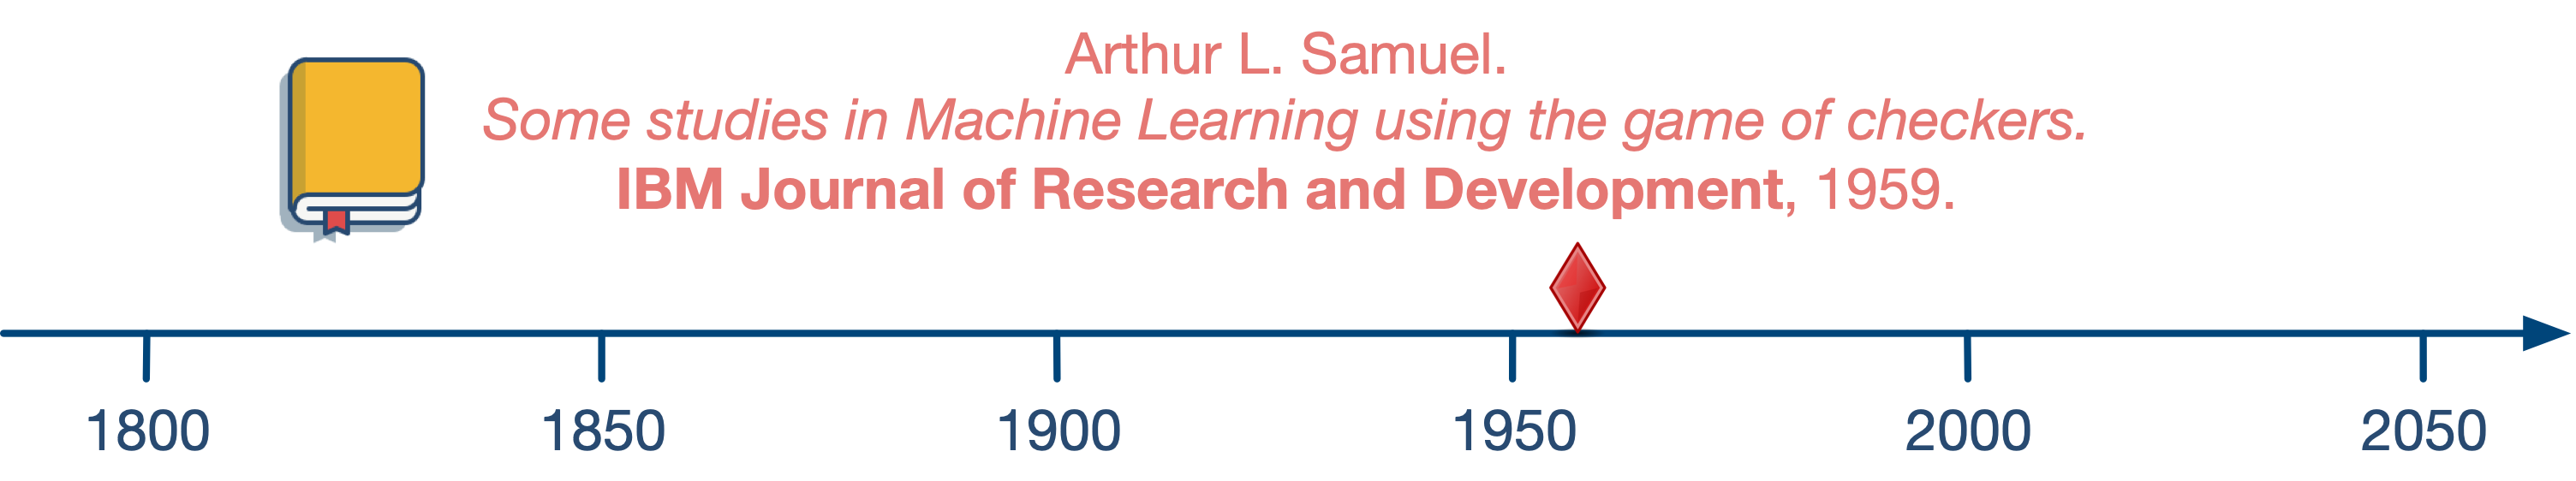
\includegraphics[width=\textwidth]{AI-timeline-1959-alt.png}
        \end{figure}
    \end{minipage}
    \\\vspace*{.3cm}
    \begin{minipage}[t]{\textwidth}
        \begin{minipage}[t]{0.6\textwidth}
            \begin{itemize}[leftmargin=10pt,align=right]
                \onslide<2->\item[\alert{\faArrowCircleRight}] Nato all'inizio del primo declino della AI
                \onslide<3->\begin{itemize}[leftmargin=10pt,align=right]
                                \item[\alert{\faArrowCircleRight}] Riprende l'eredità di Rosenblatt (algoritmo di apprendimento del \emph{perceptron})
                                \onslide<4->\item[\alert{\faArrowCircleRight}] Insieme di metodologie che
                                \begin{itemize}[leftmargin=10pt,align=right]
                                    \item[\alert{\faArrowCircleRight}] scoprono \alert{modelli} (regolarit\'{a} o \alert{pattern}) nei dati
                                    \item[\alert{\faArrowCircleRight}] predicono comportamenti o prendono decisioni sulla base di nuovi dati
                                \end{itemize}
                \end{itemize}
            \end{itemize}
            \onslide<4->
            \begin{minipage}[t]{\textwidth}
                \renewcommand{\epigraphsize}{\scriptsize}
                \setlength{\afterepigraphskip}{0pt}
                \setlength{\beforeepigraphskip}{0pt}
                \setlength{\epigraphwidth}{0.9\textwidth}
                \epigraph{\textit{Si dice che un programma \alert{apprende} dall'esperienza $E$ con riferimento ad alcune classi di compiti $T$ e con misurazione della performance $P$, se le sue \emph{performance} nel compito $T$, come misurato da $P$, migliorano con l'esperienza $E$.}}{\textbf{Tom Mitchell, 1997}}
            \end{minipage}
        \end{minipage}
        %
        \onslide<1->
        \begin{minipage}[t]{0.4\textwidth}
            \centering
            \begin{figure}[ht]
                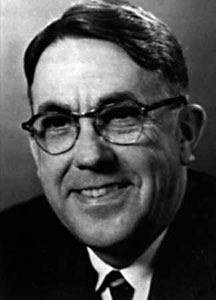
\includegraphics[width=.55\textwidth]{Arthur_Samuel.jpg}
                {\tiny\\Arthur Samuel\\\vspace*{-1pt}\textit{\textcopyright HistoryOfInformation}}
            \end{figure}
        \end{minipage}
    \end{minipage}
}
\end{frame}
%
\begin{frame}[t] \frametitle{\emph{Workflow} processo di \emph{Machine Learning}}
    \only<1|handout:1>{
    \framesubtitle{Visione semplificata}
    }
 \only<2|handout:2>{
    \framesubtitle{Visione dettagliata}
 }
 \only<3|handout:3>{
    \framesubtitle{Come avviene l'apprendimento?}
 }   
\only<1|handout:1>{
    \begin{center}
        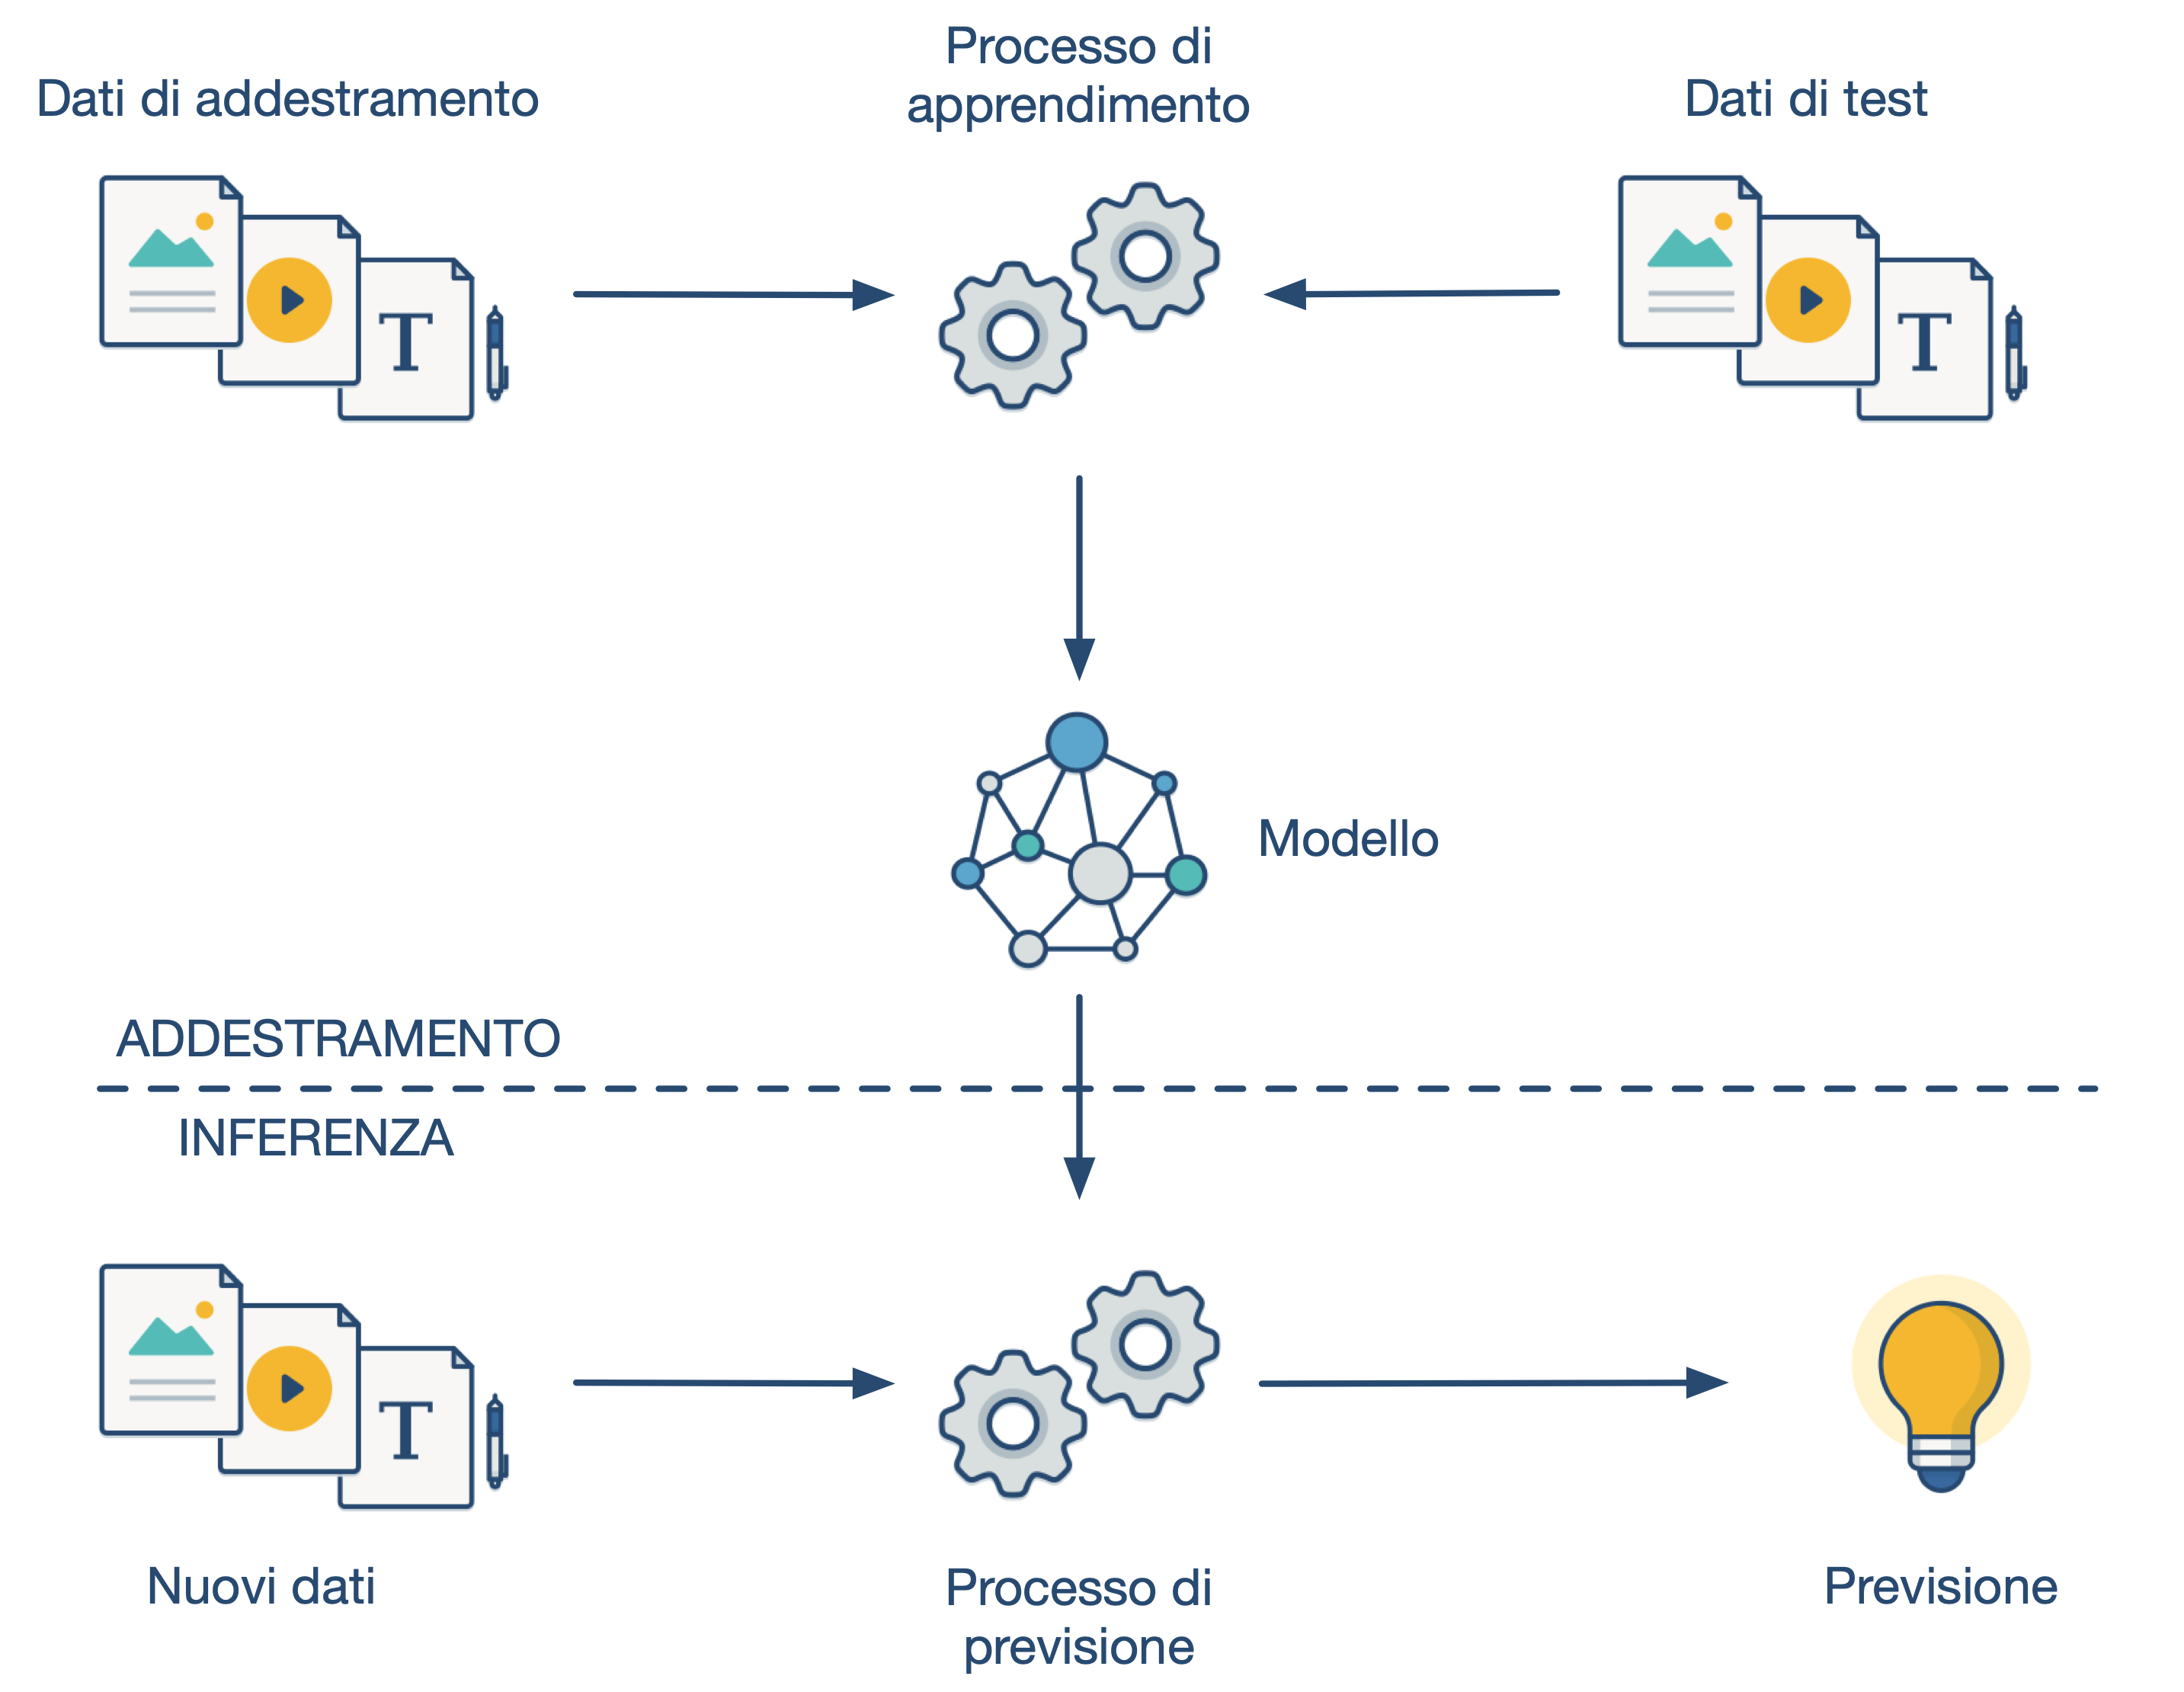
\includegraphics[height=6cm,keepaspectratio]{MLWithoutParameters.png}
    \end{center}
    \begin{flushright}
        {\tiny\textit{\textcopyright Simone Scannapieco}}
    \end{flushright}
}
\only<2|handout:2>{
    \begin{center}
        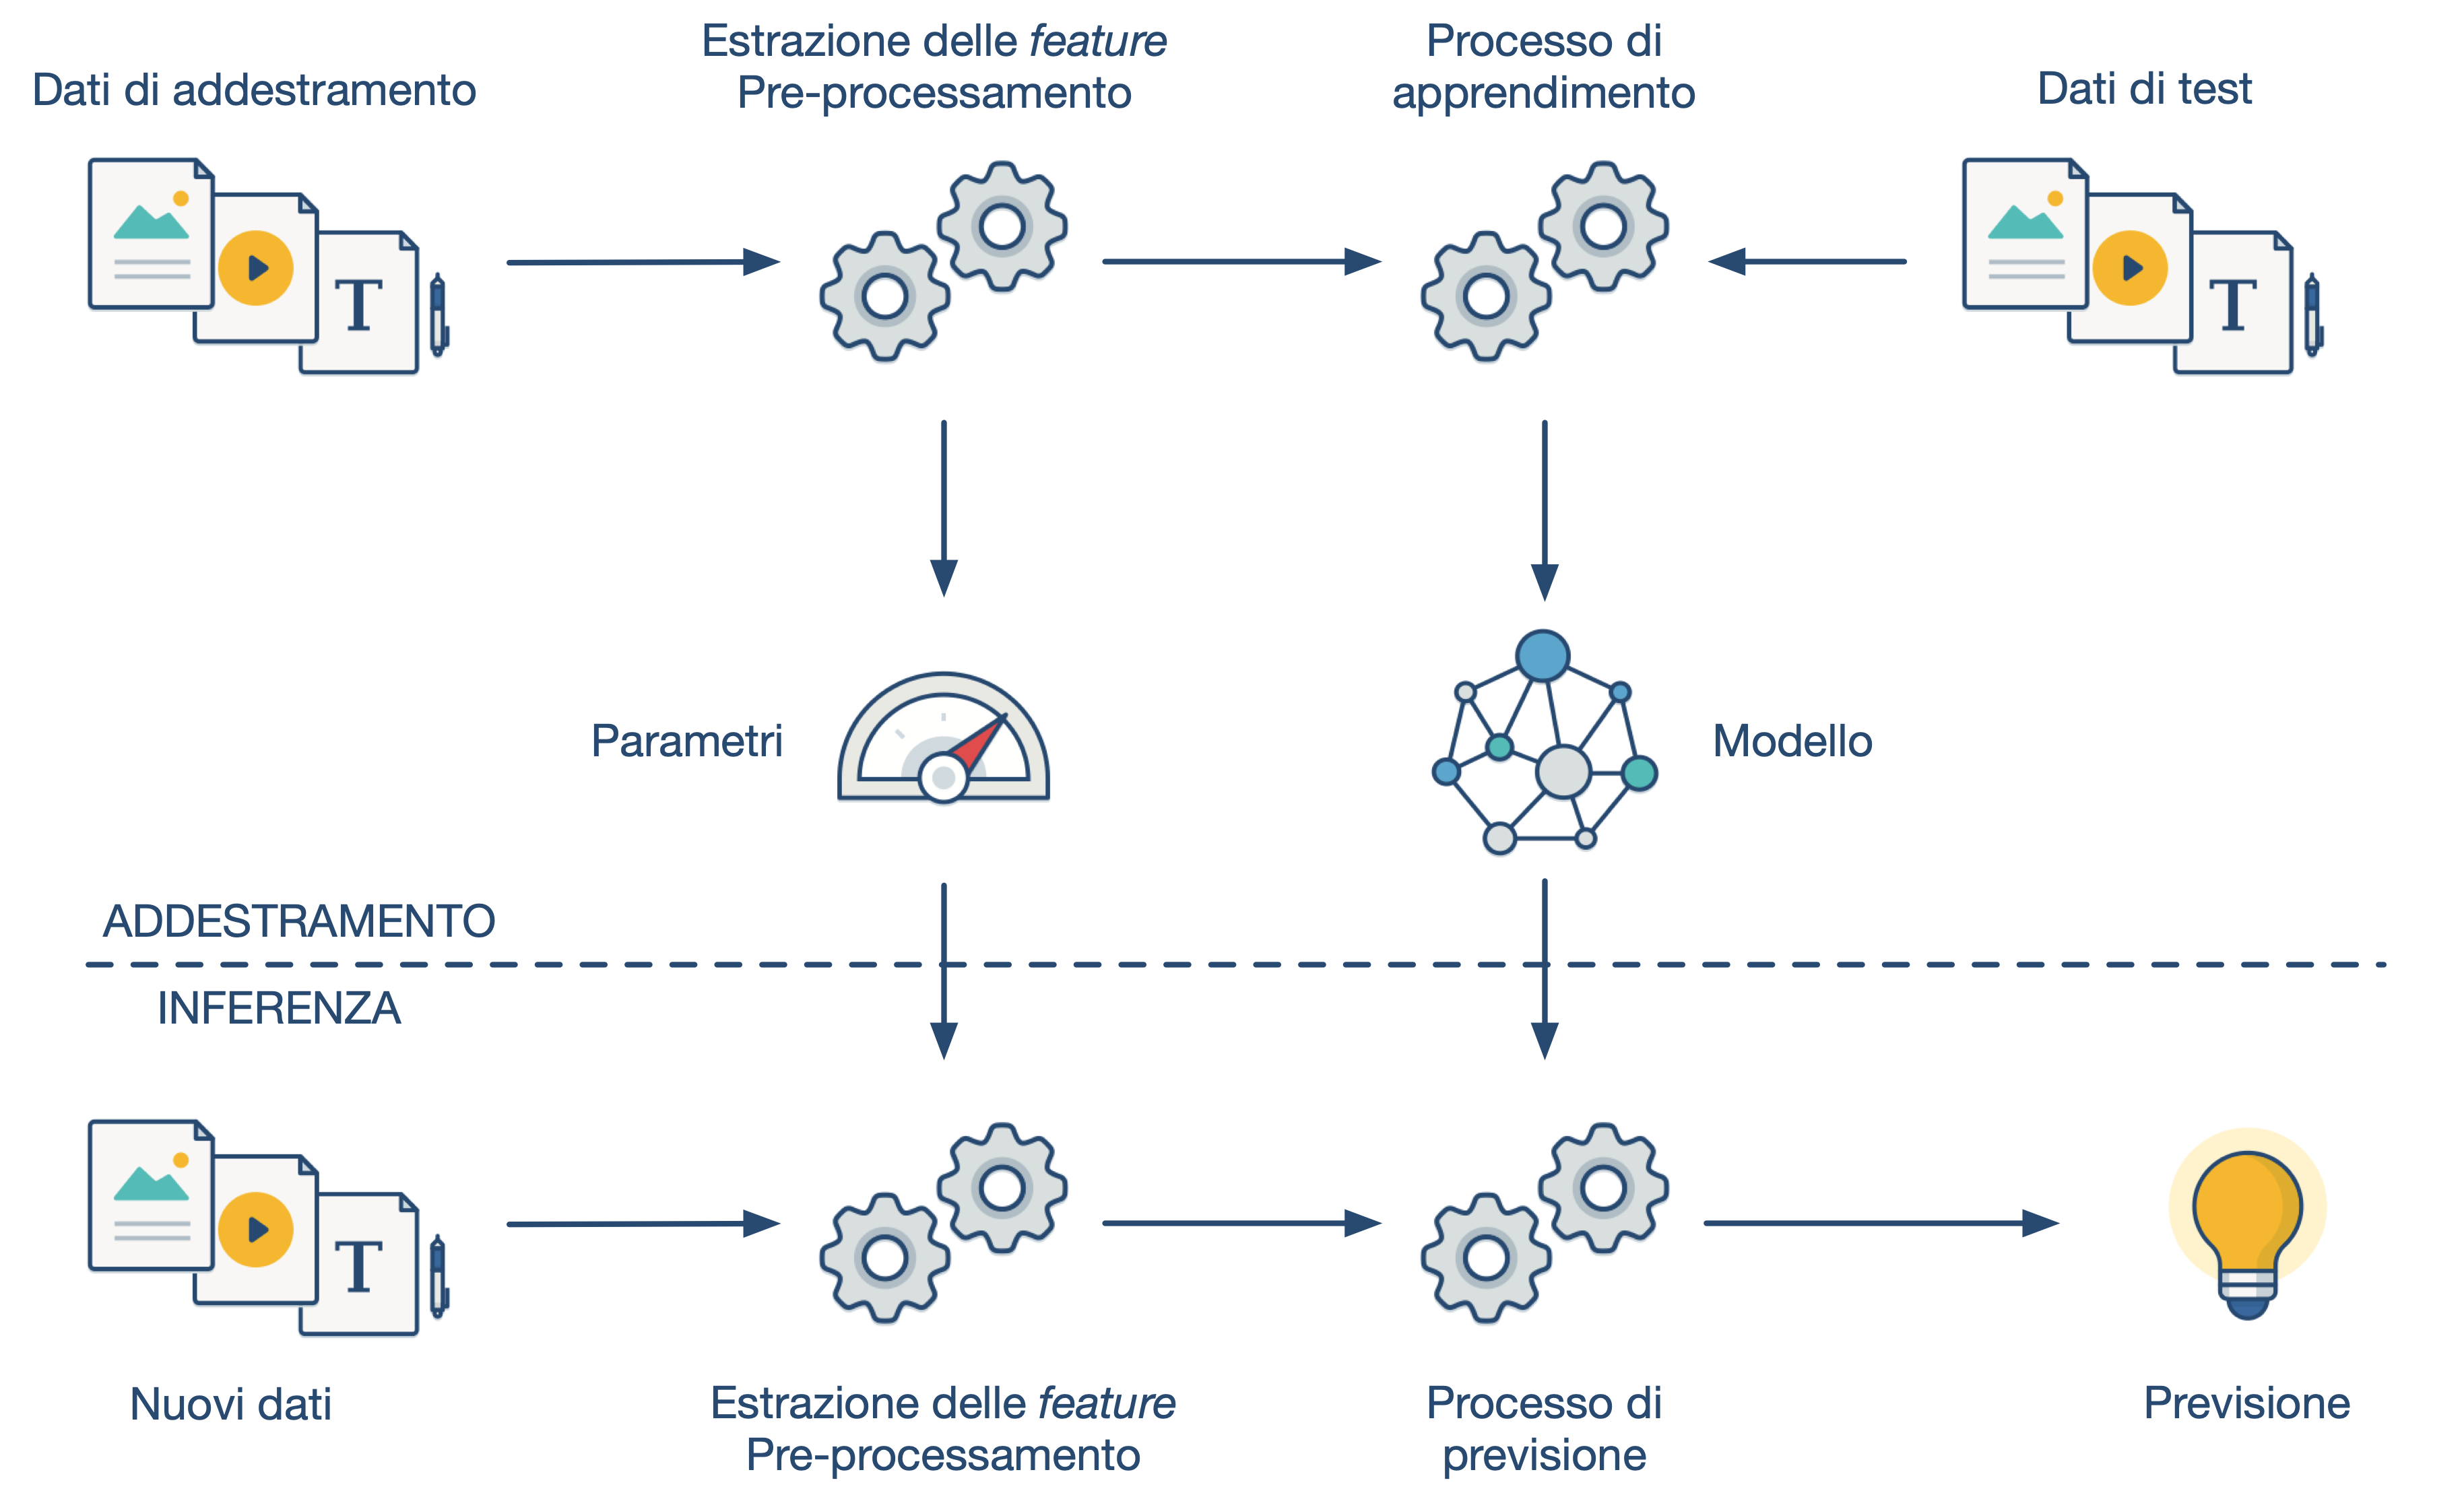
\includegraphics[height=6cm,keepaspectratio]{MLWithParameters.png}
    \end{center}
    \begin{flushright}
        {\tiny\textit{\textcopyright Simone Scannapieco}}
    \end{flushright}
}
\only<3|handout:3>{
    \begin{center}
        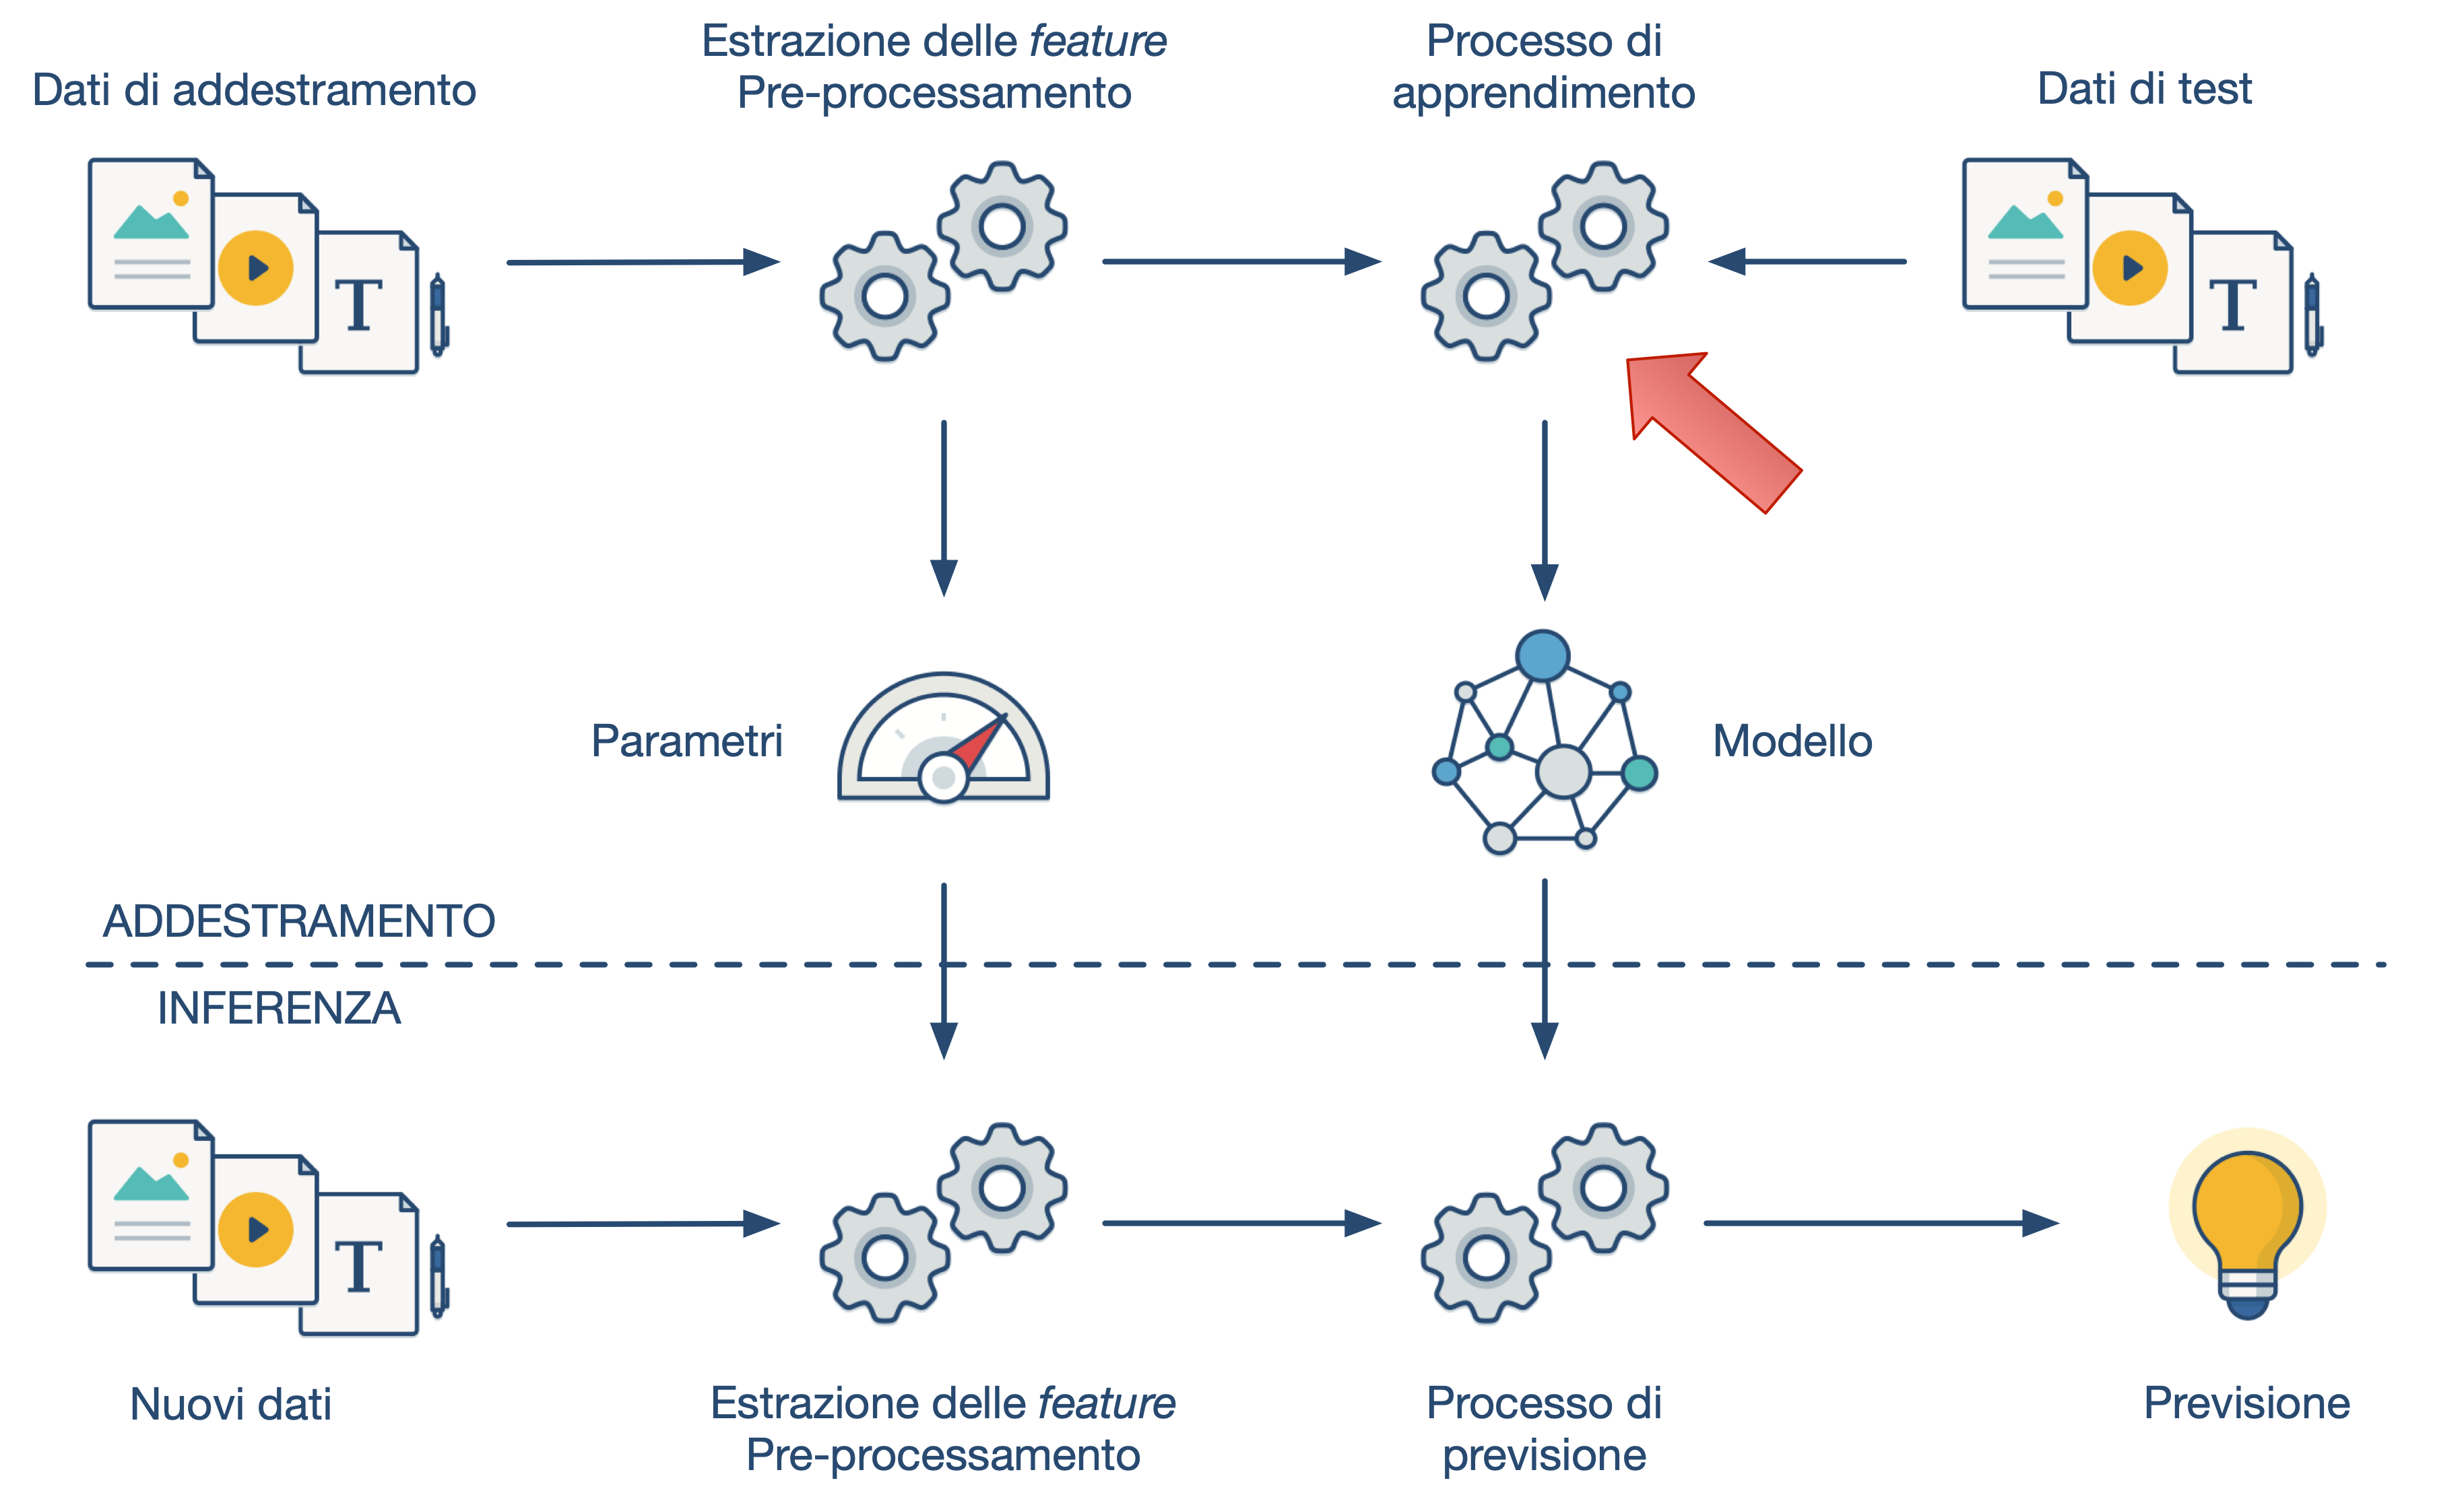
\includegraphics[height=6cm,keepaspectratio]{MLWithParametersAndArrowOnMLP.png}
    \end{center}
    \begin{flushright}
        {\tiny\textit{\textcopyright Simone Scannapieco}}
    \end{flushright}
}
\end{frame}
%
\begin{frame}[t] \frametitle{Processi di apprendimento}
    \framesubtitle{Classificazione canonica}  
\only<1|handout:0>{
    \begin{center}
        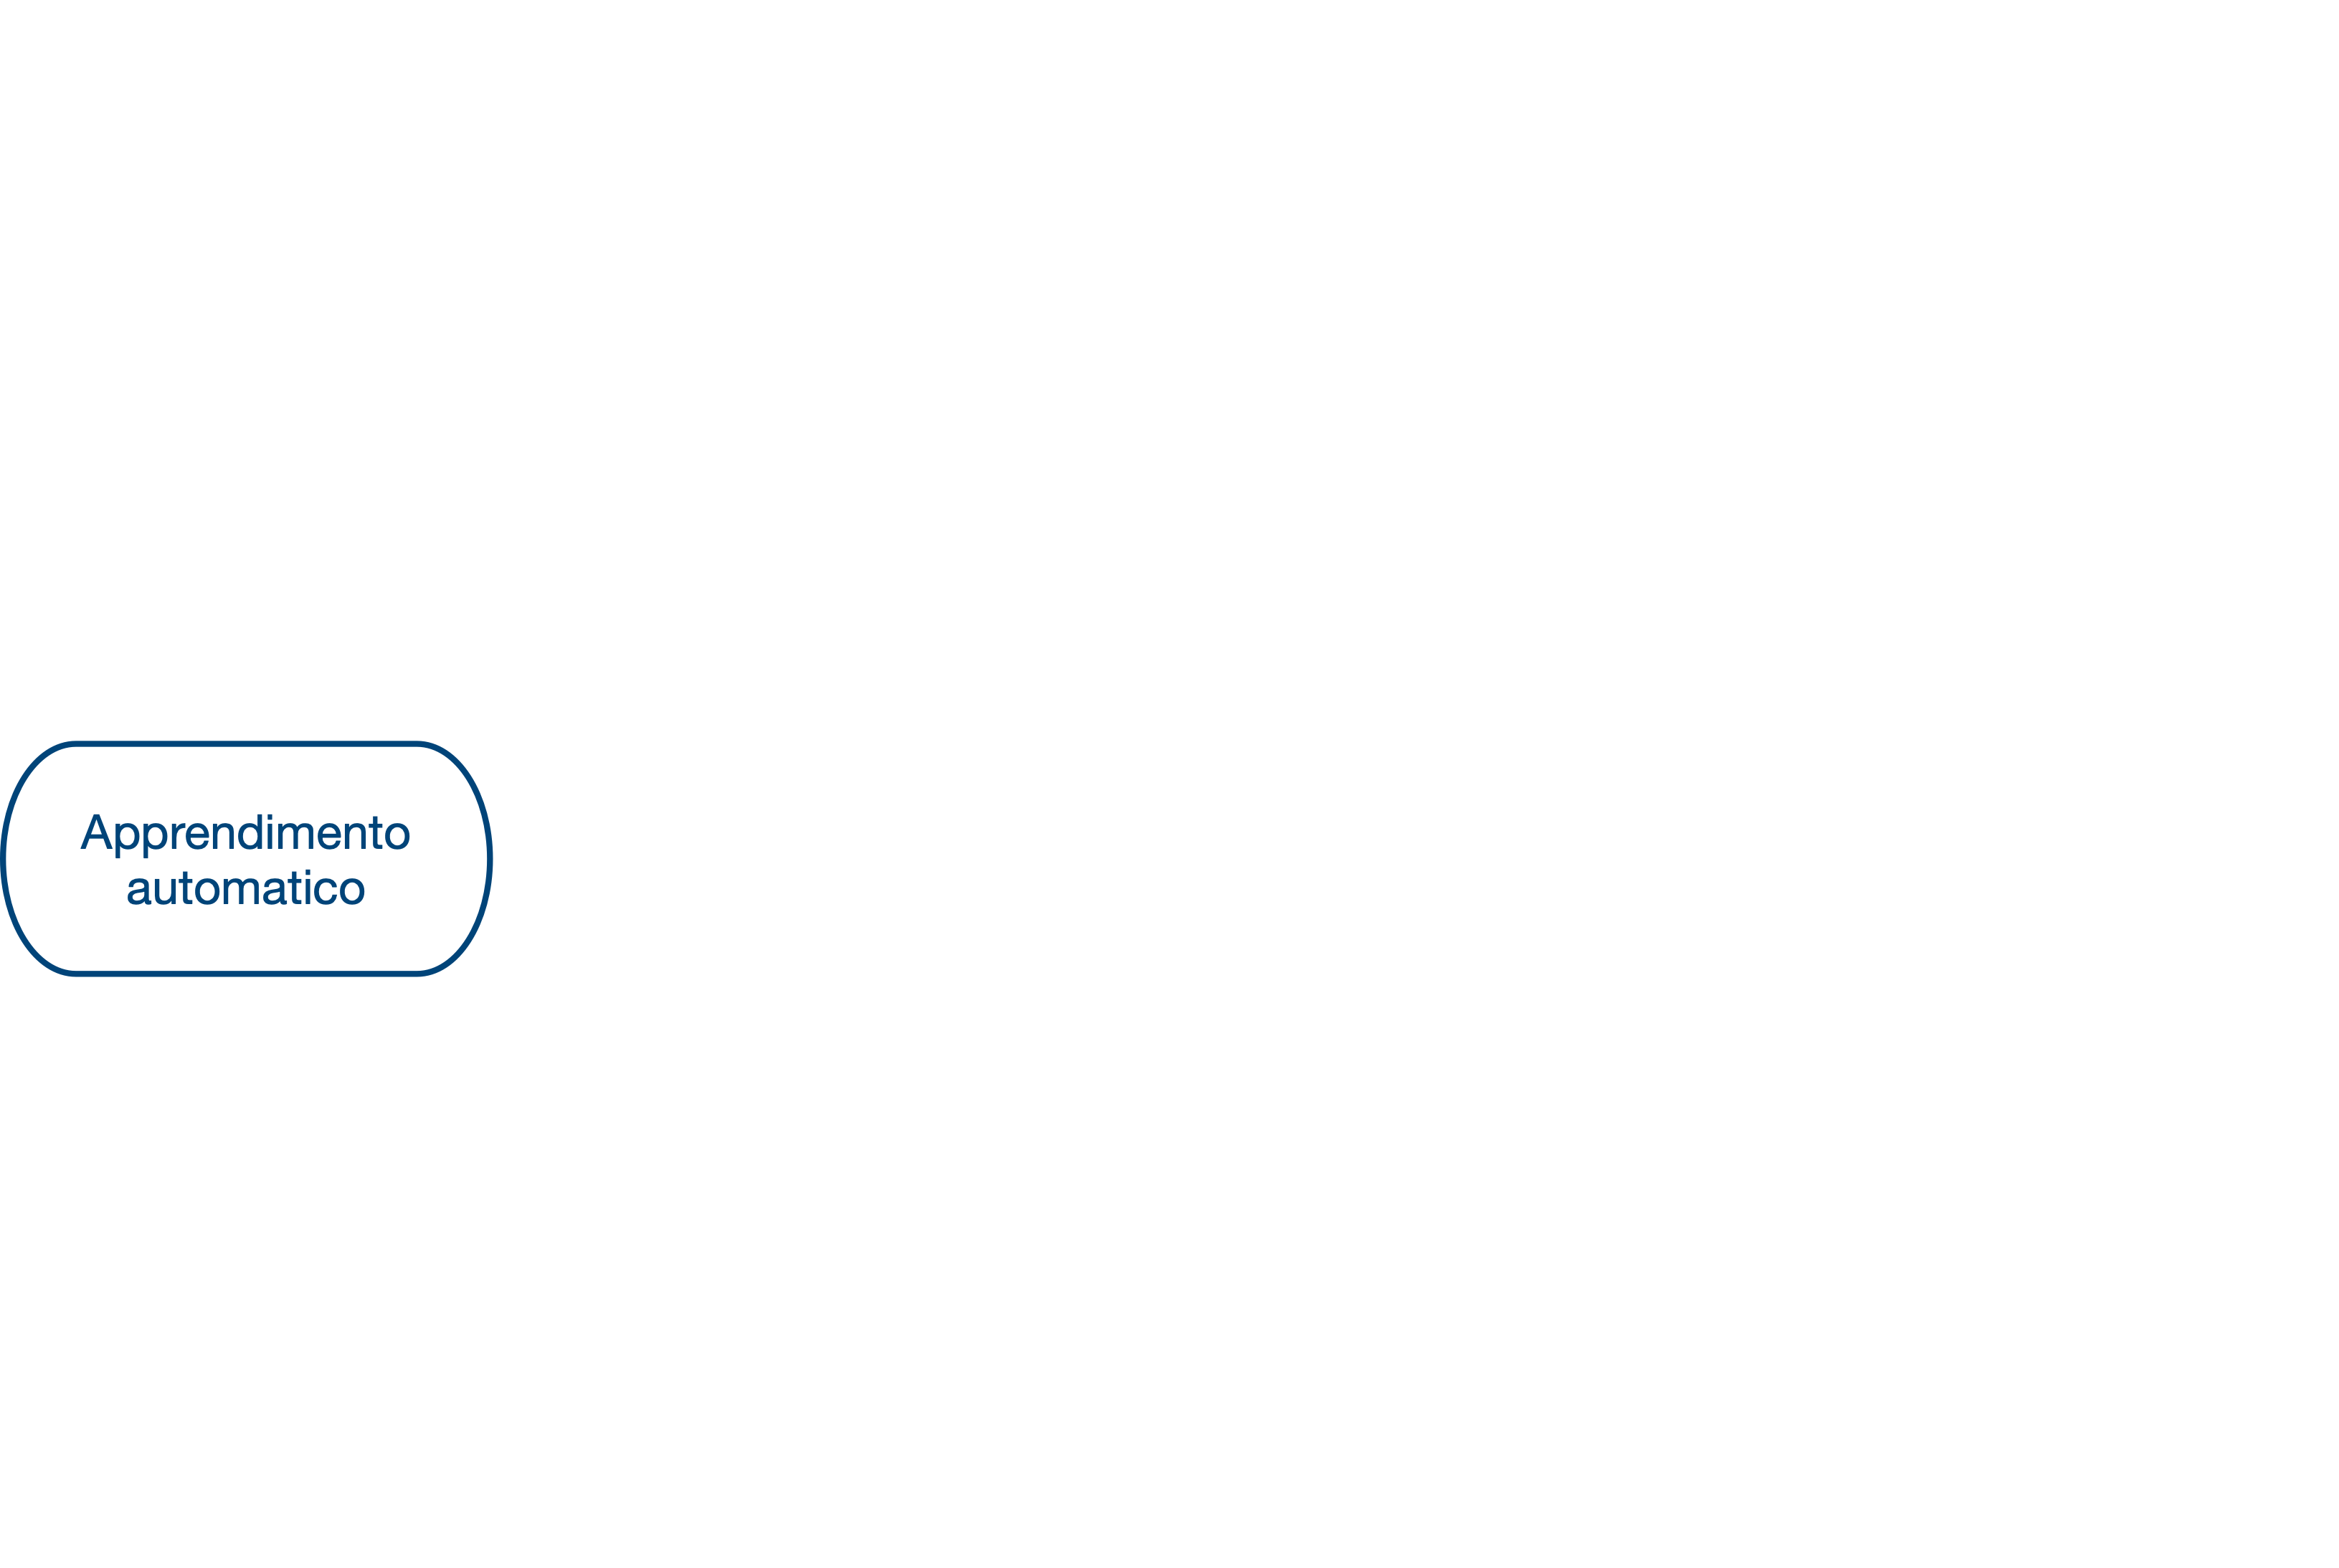
\includegraphics[scale=.2]{AA.png}
    \end{center}
    \begin{flushright}
        {\tiny\textit{\textcopyright Simone Scannapieco}}
    \end{flushright}
}
\only<2|handout:1>{
    \begin{center}
        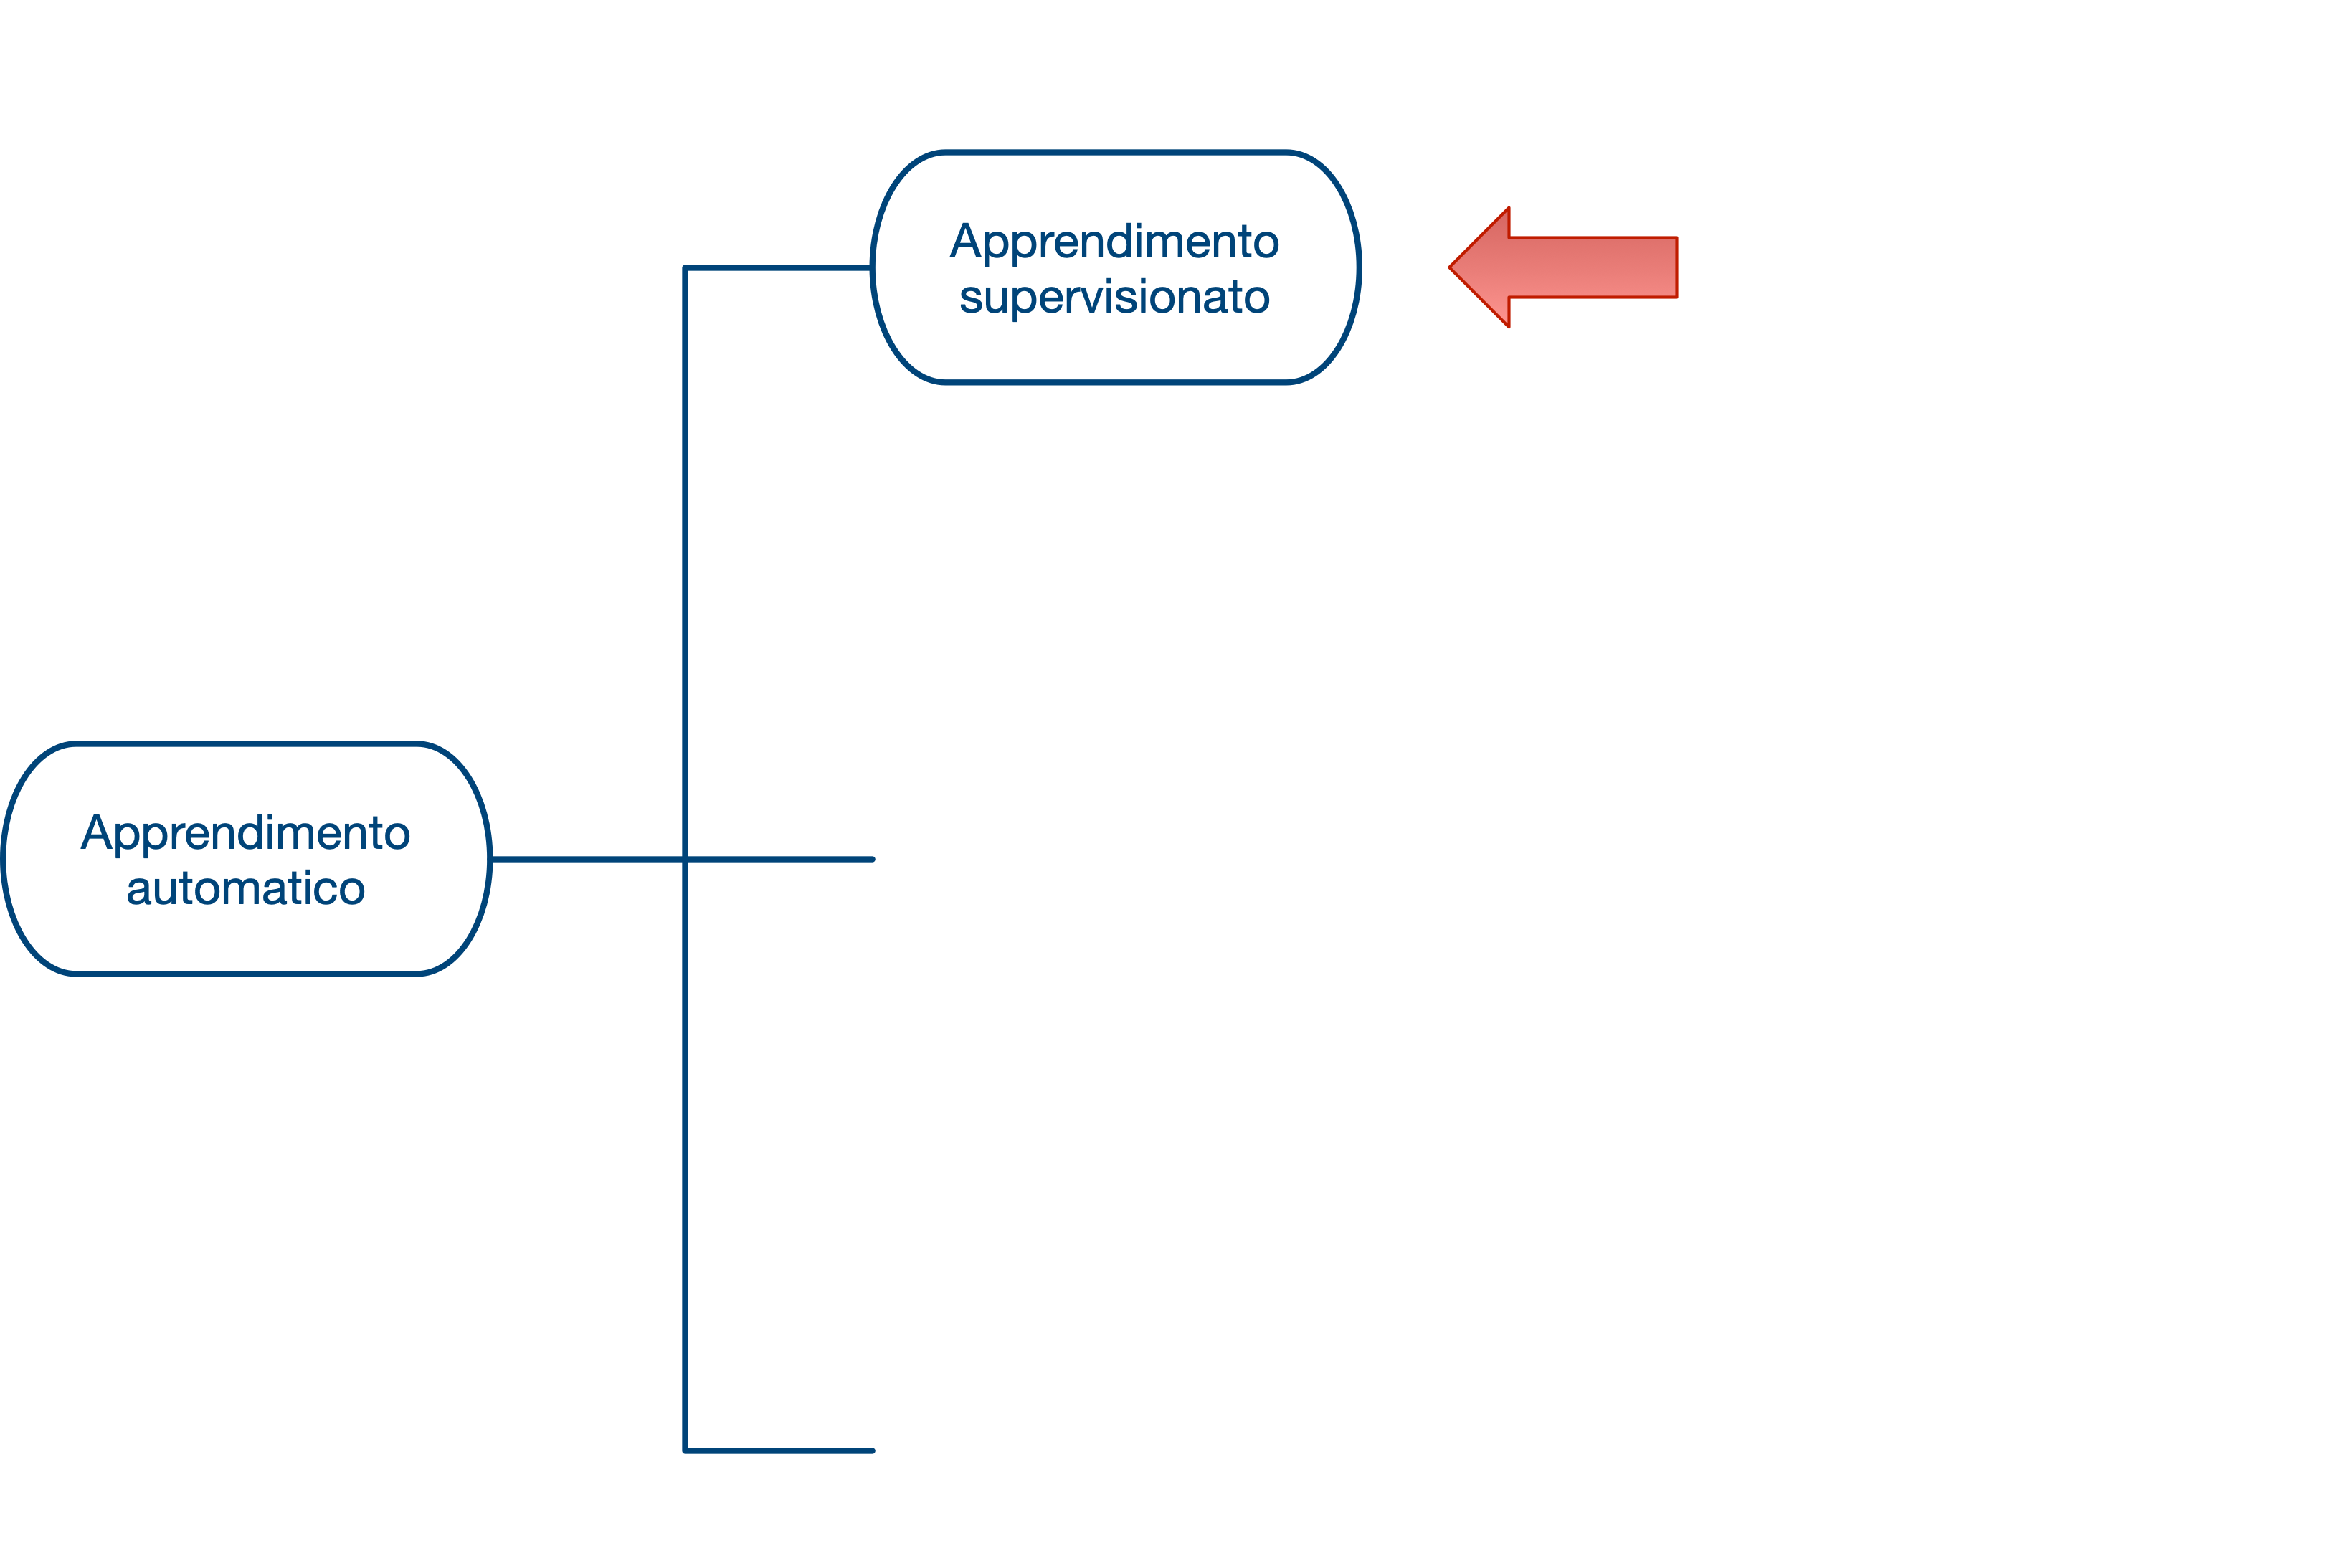
\includegraphics[scale=.2]{AAeAS.png}
    \end{center}
    \begin{flushright}
        {\tiny\textit{\textcopyright Simone Scannapieco}}
    \end{flushright}
    {\footnotesize
        \begin{itemize}[leftmargin=10pt,align=right]
            \item[\alert{\faArrowCircleRight}] Per ogni dato abbiamo il valore che desideriamo venisse predetto dal modello (\alert{etichetta})
            \item[\alert{\faArrowCircleRight}] Supervisore che etichetta ogni dato di addestramento
            \item[\alert{\faArrowCircleRight}] Ricerca di un modello che realizzi la corrispondenza dato-etichetta corrispondente
        \end{itemize}
    }
}
\only<3|handout:2>{
    \begin{center}
        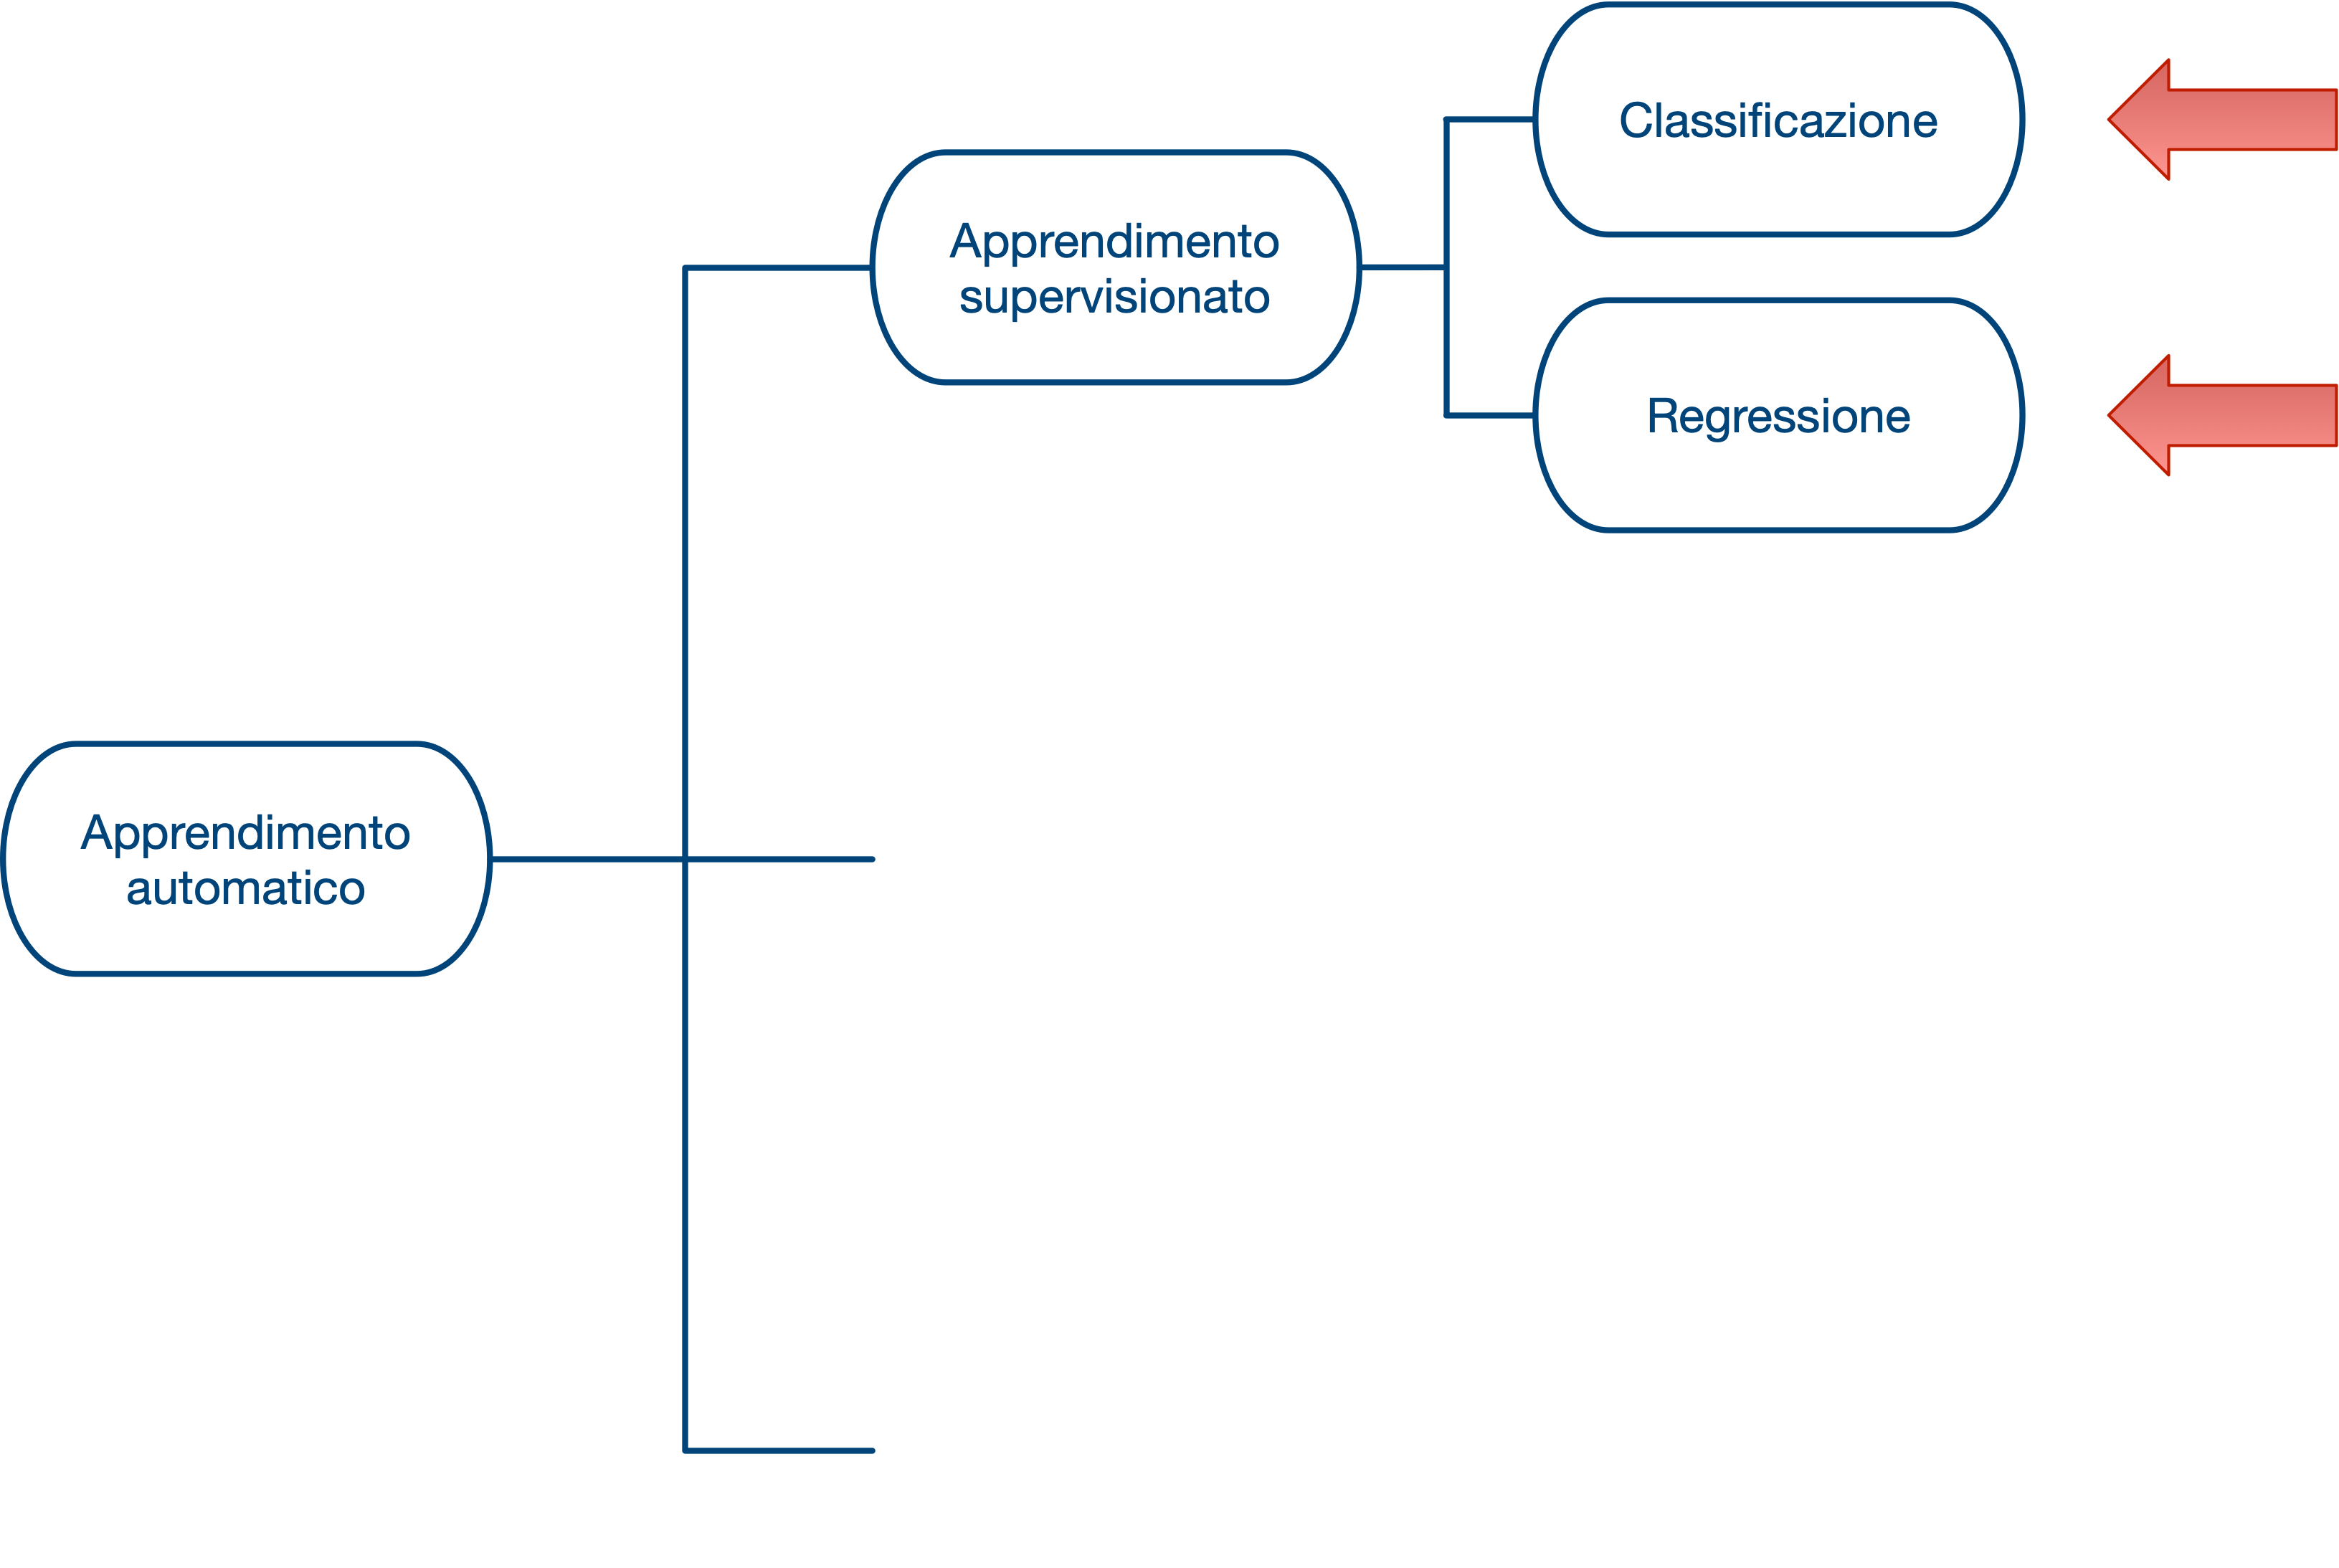
\includegraphics[scale=.2]{AAeASeSottotipi.png}
    \end{center}
    \begin{flushright}
        {\tiny\textit{\textcopyright Simone Scannapieco}}
    \end{flushright}
    {\footnotesize
        \begin{itemize}[leftmargin=10pt,align=right]
            \item[\alert{\faArrowCircleRight}] \alert{Classificazione} quando il numero di etichette è finito (es. identificazione di oggetti)
            \item[\alert{\faArrowCircleRight}] \alert{Regressione} quando l'etichetta ha un numero infinito di valori (es. previsione di un numero reale)
        \end{itemize}
    }
}
\only<4|handout:3>{
    \begin{center}
        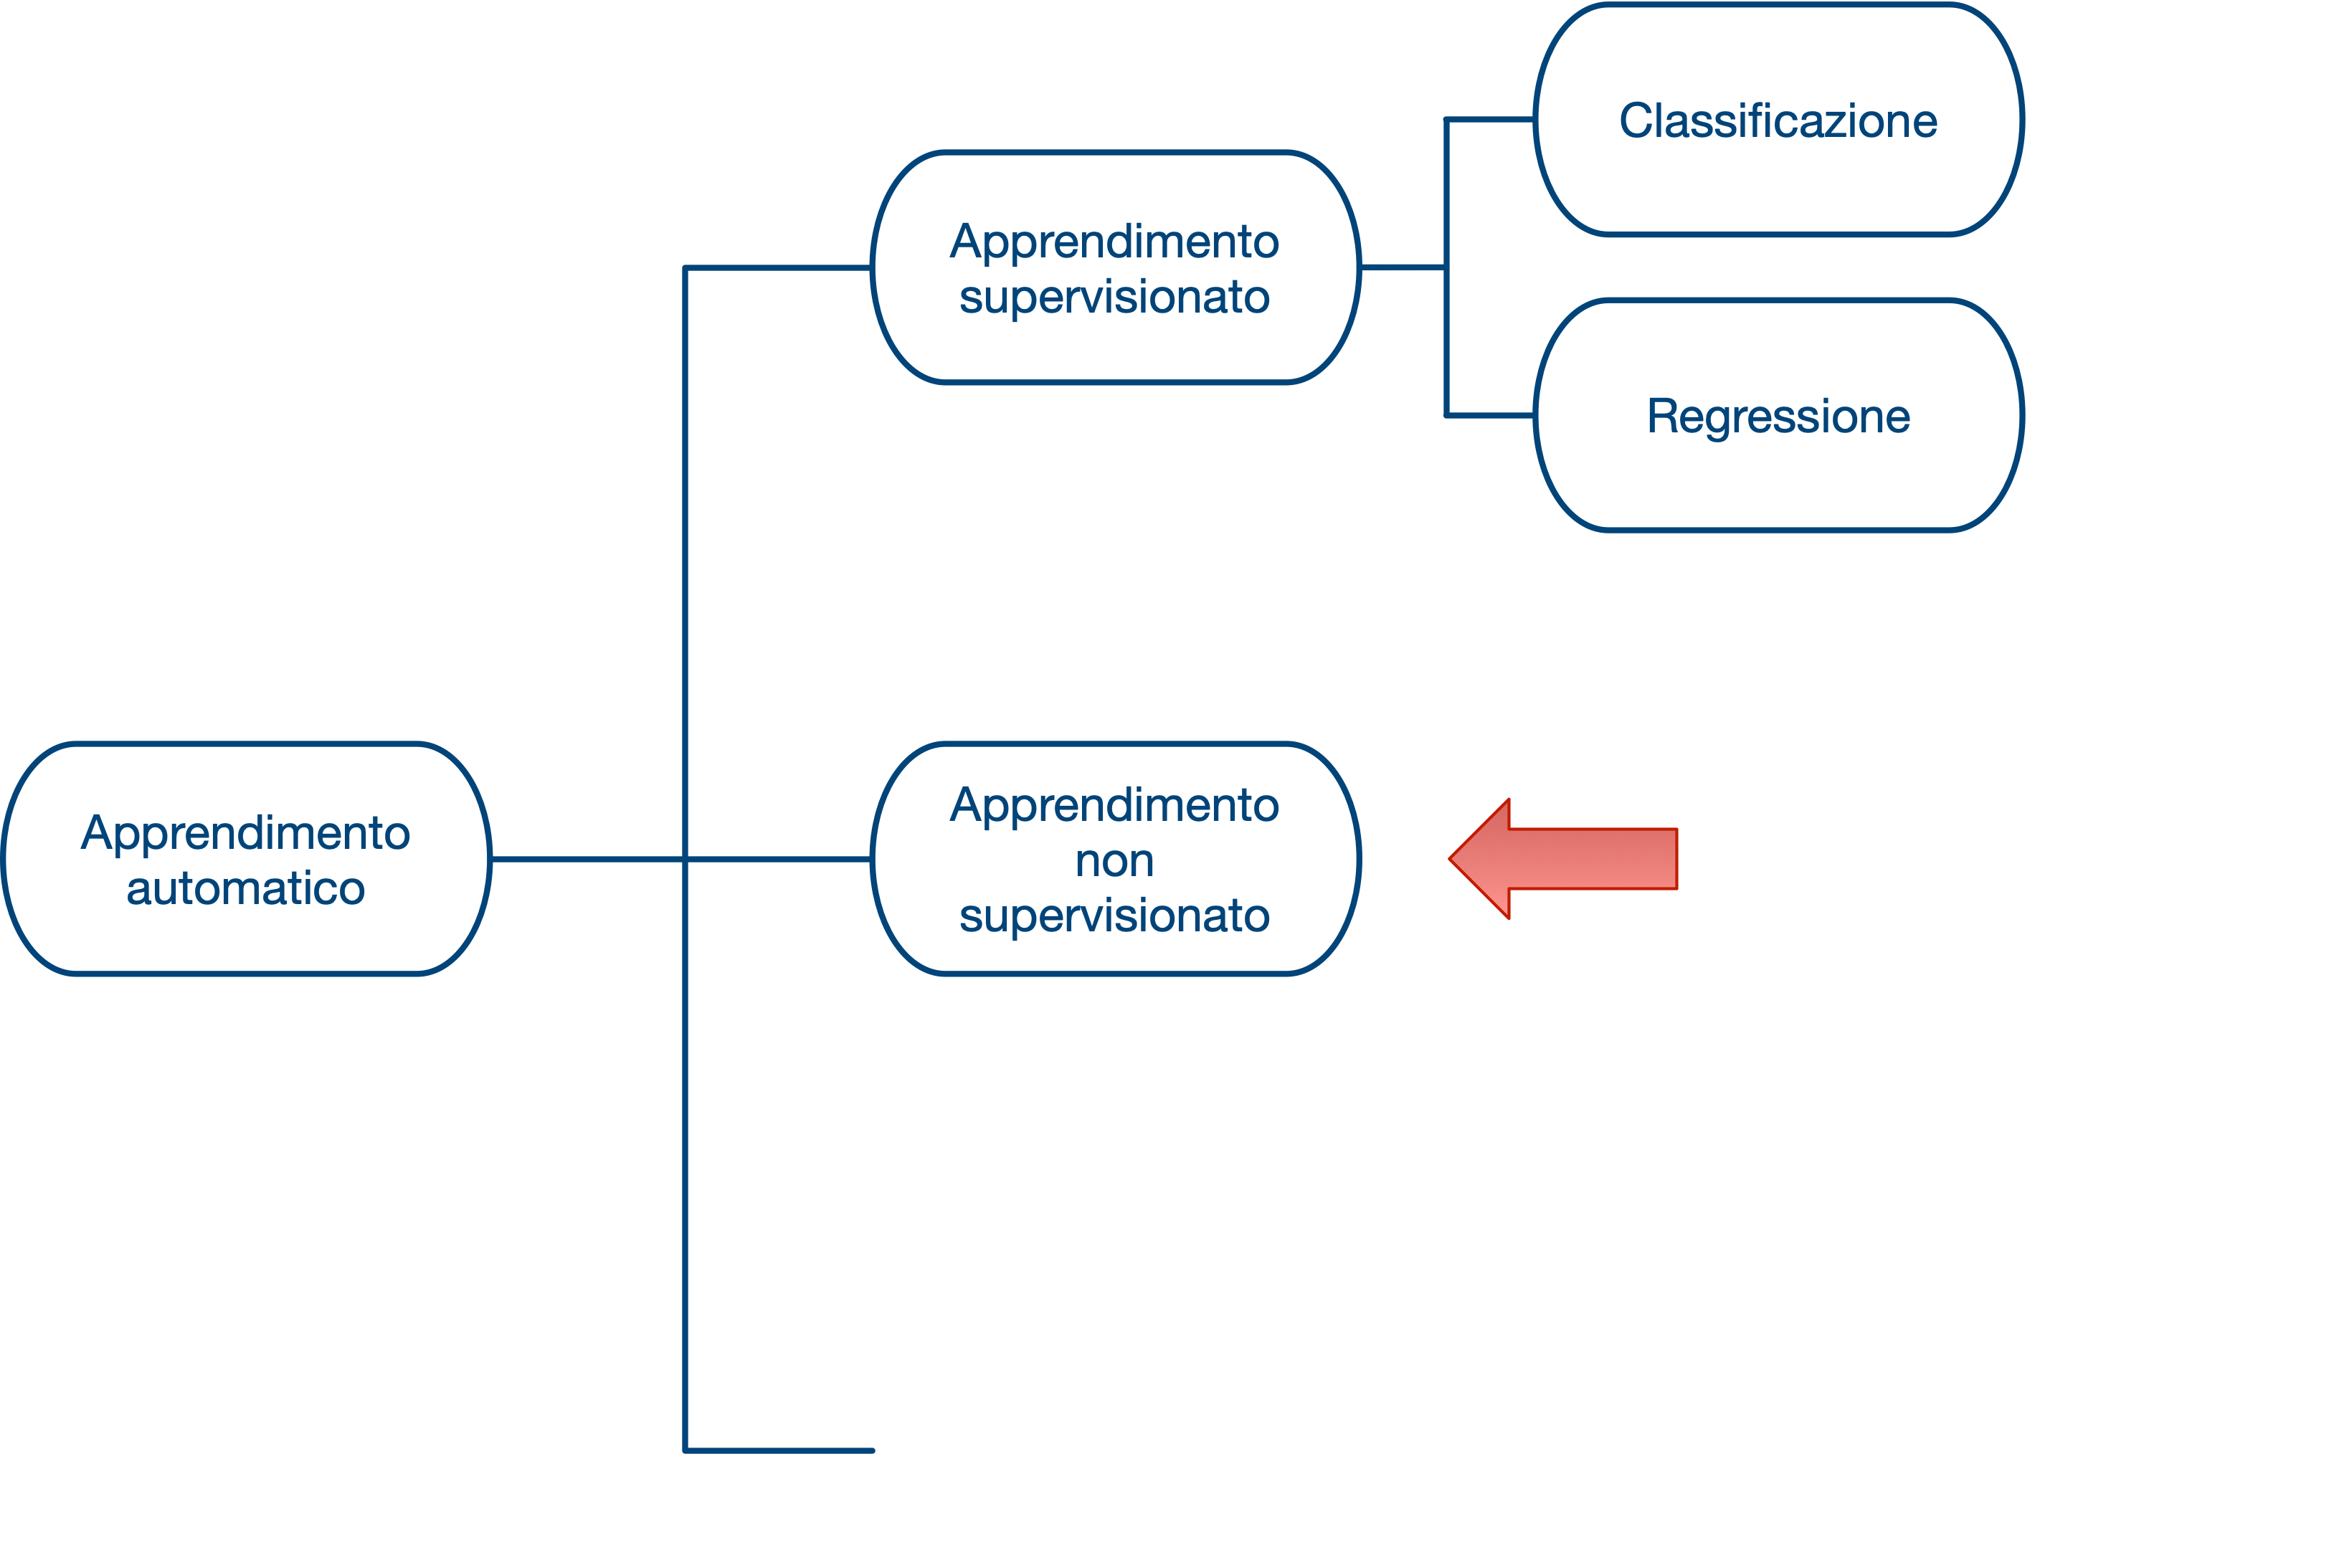
\includegraphics[scale=.2]{AAeASeANS.png}
    \end{center}
    \begin{flushright}
        {\tiny\textit{\textcopyright Simone Scannapieco}}
    \end{flushright}
    {\footnotesize
        \begin{itemize}[leftmargin=10pt,align=right]
            \item[\alert{\faArrowCircleRight}] Nessun supervisore etichetta i dati
            \item[\alert{\faArrowCircleRight}] Non esiste una etichetta da predire
            \item[\alert{\faArrowCircleRight}] Il \emph{focus} è su come (e quali) dati sono relazionati fra loro (\alert{similarità})
        \end{itemize}
    }
}
\only<5|handout:4>{
    \begin{center}
        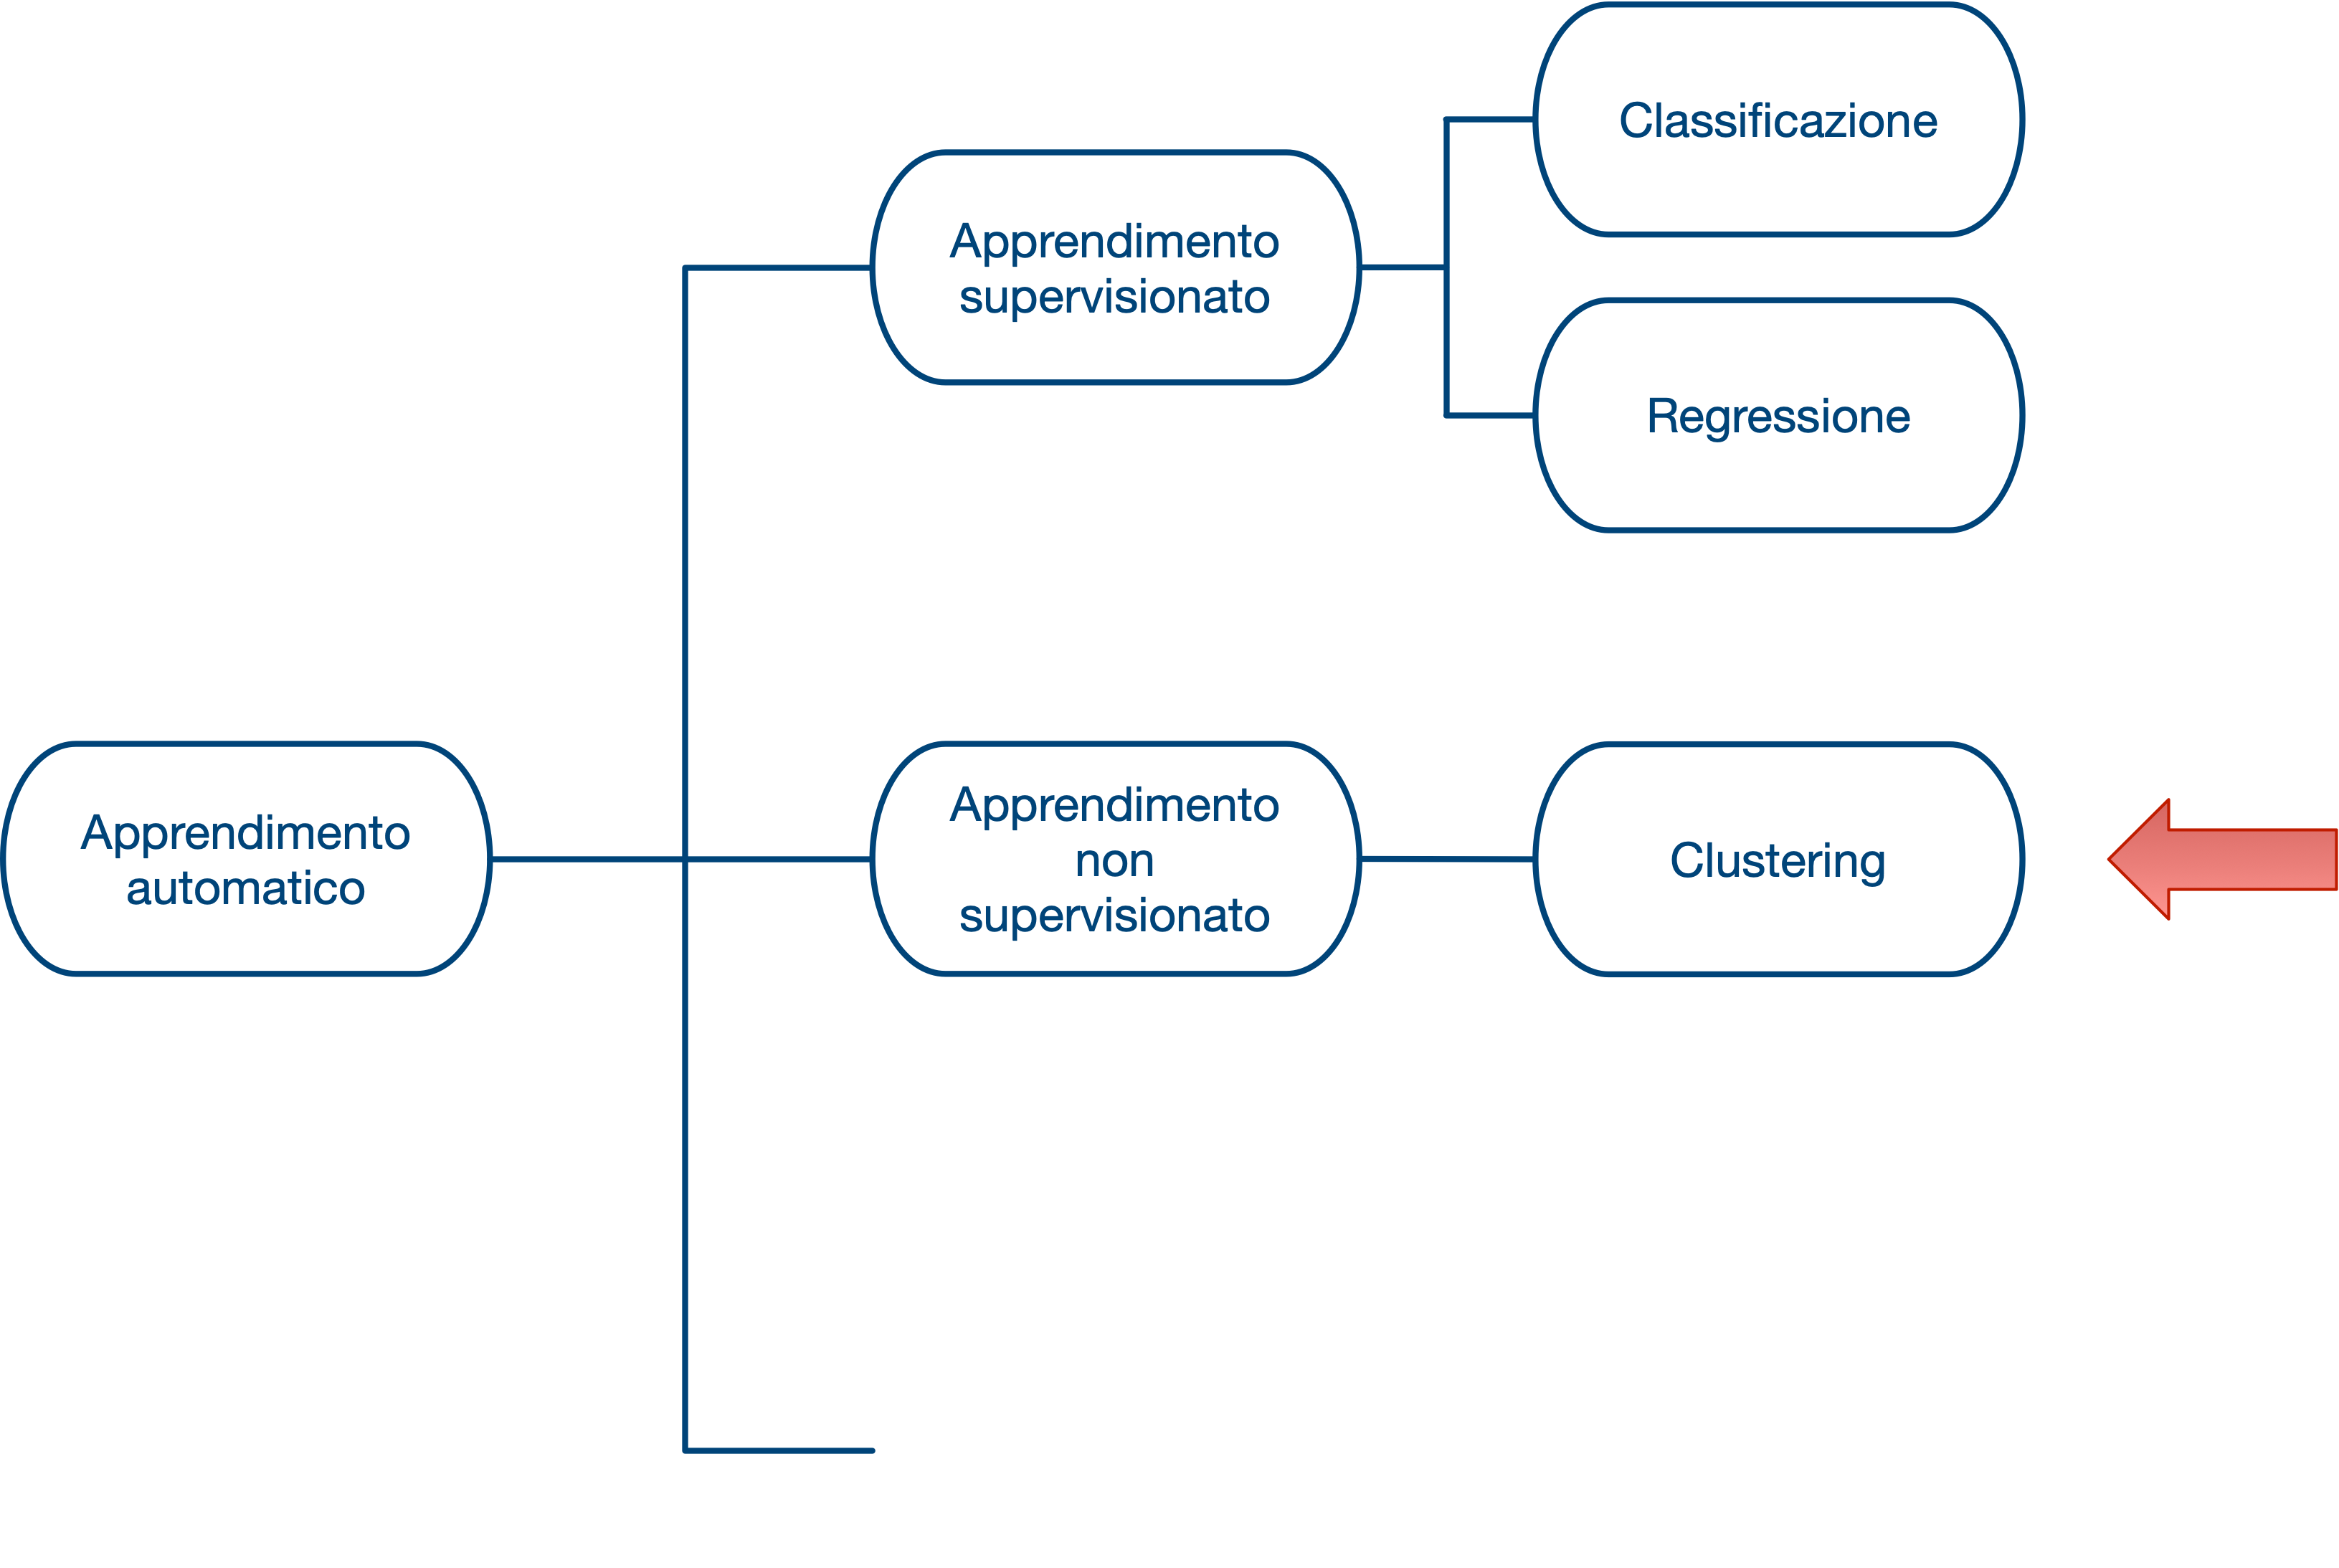
\includegraphics[scale=.2]{AAeANSeSottotipi.png}
    \end{center}
    \begin{flushright}
        {\tiny\textit{\textcopyright Simone Scannapieco}}
    \end{flushright}
    {\footnotesize
        \begin{itemize}[leftmargin=10pt,align=right]
            \item[\alert{\faArrowCircleRight}] \emph{Clustering} per identificare gruppi disgiunti (o meno)
        \end{itemize}
    }
}
\only<6|handout:5>{
    \begin{center}
        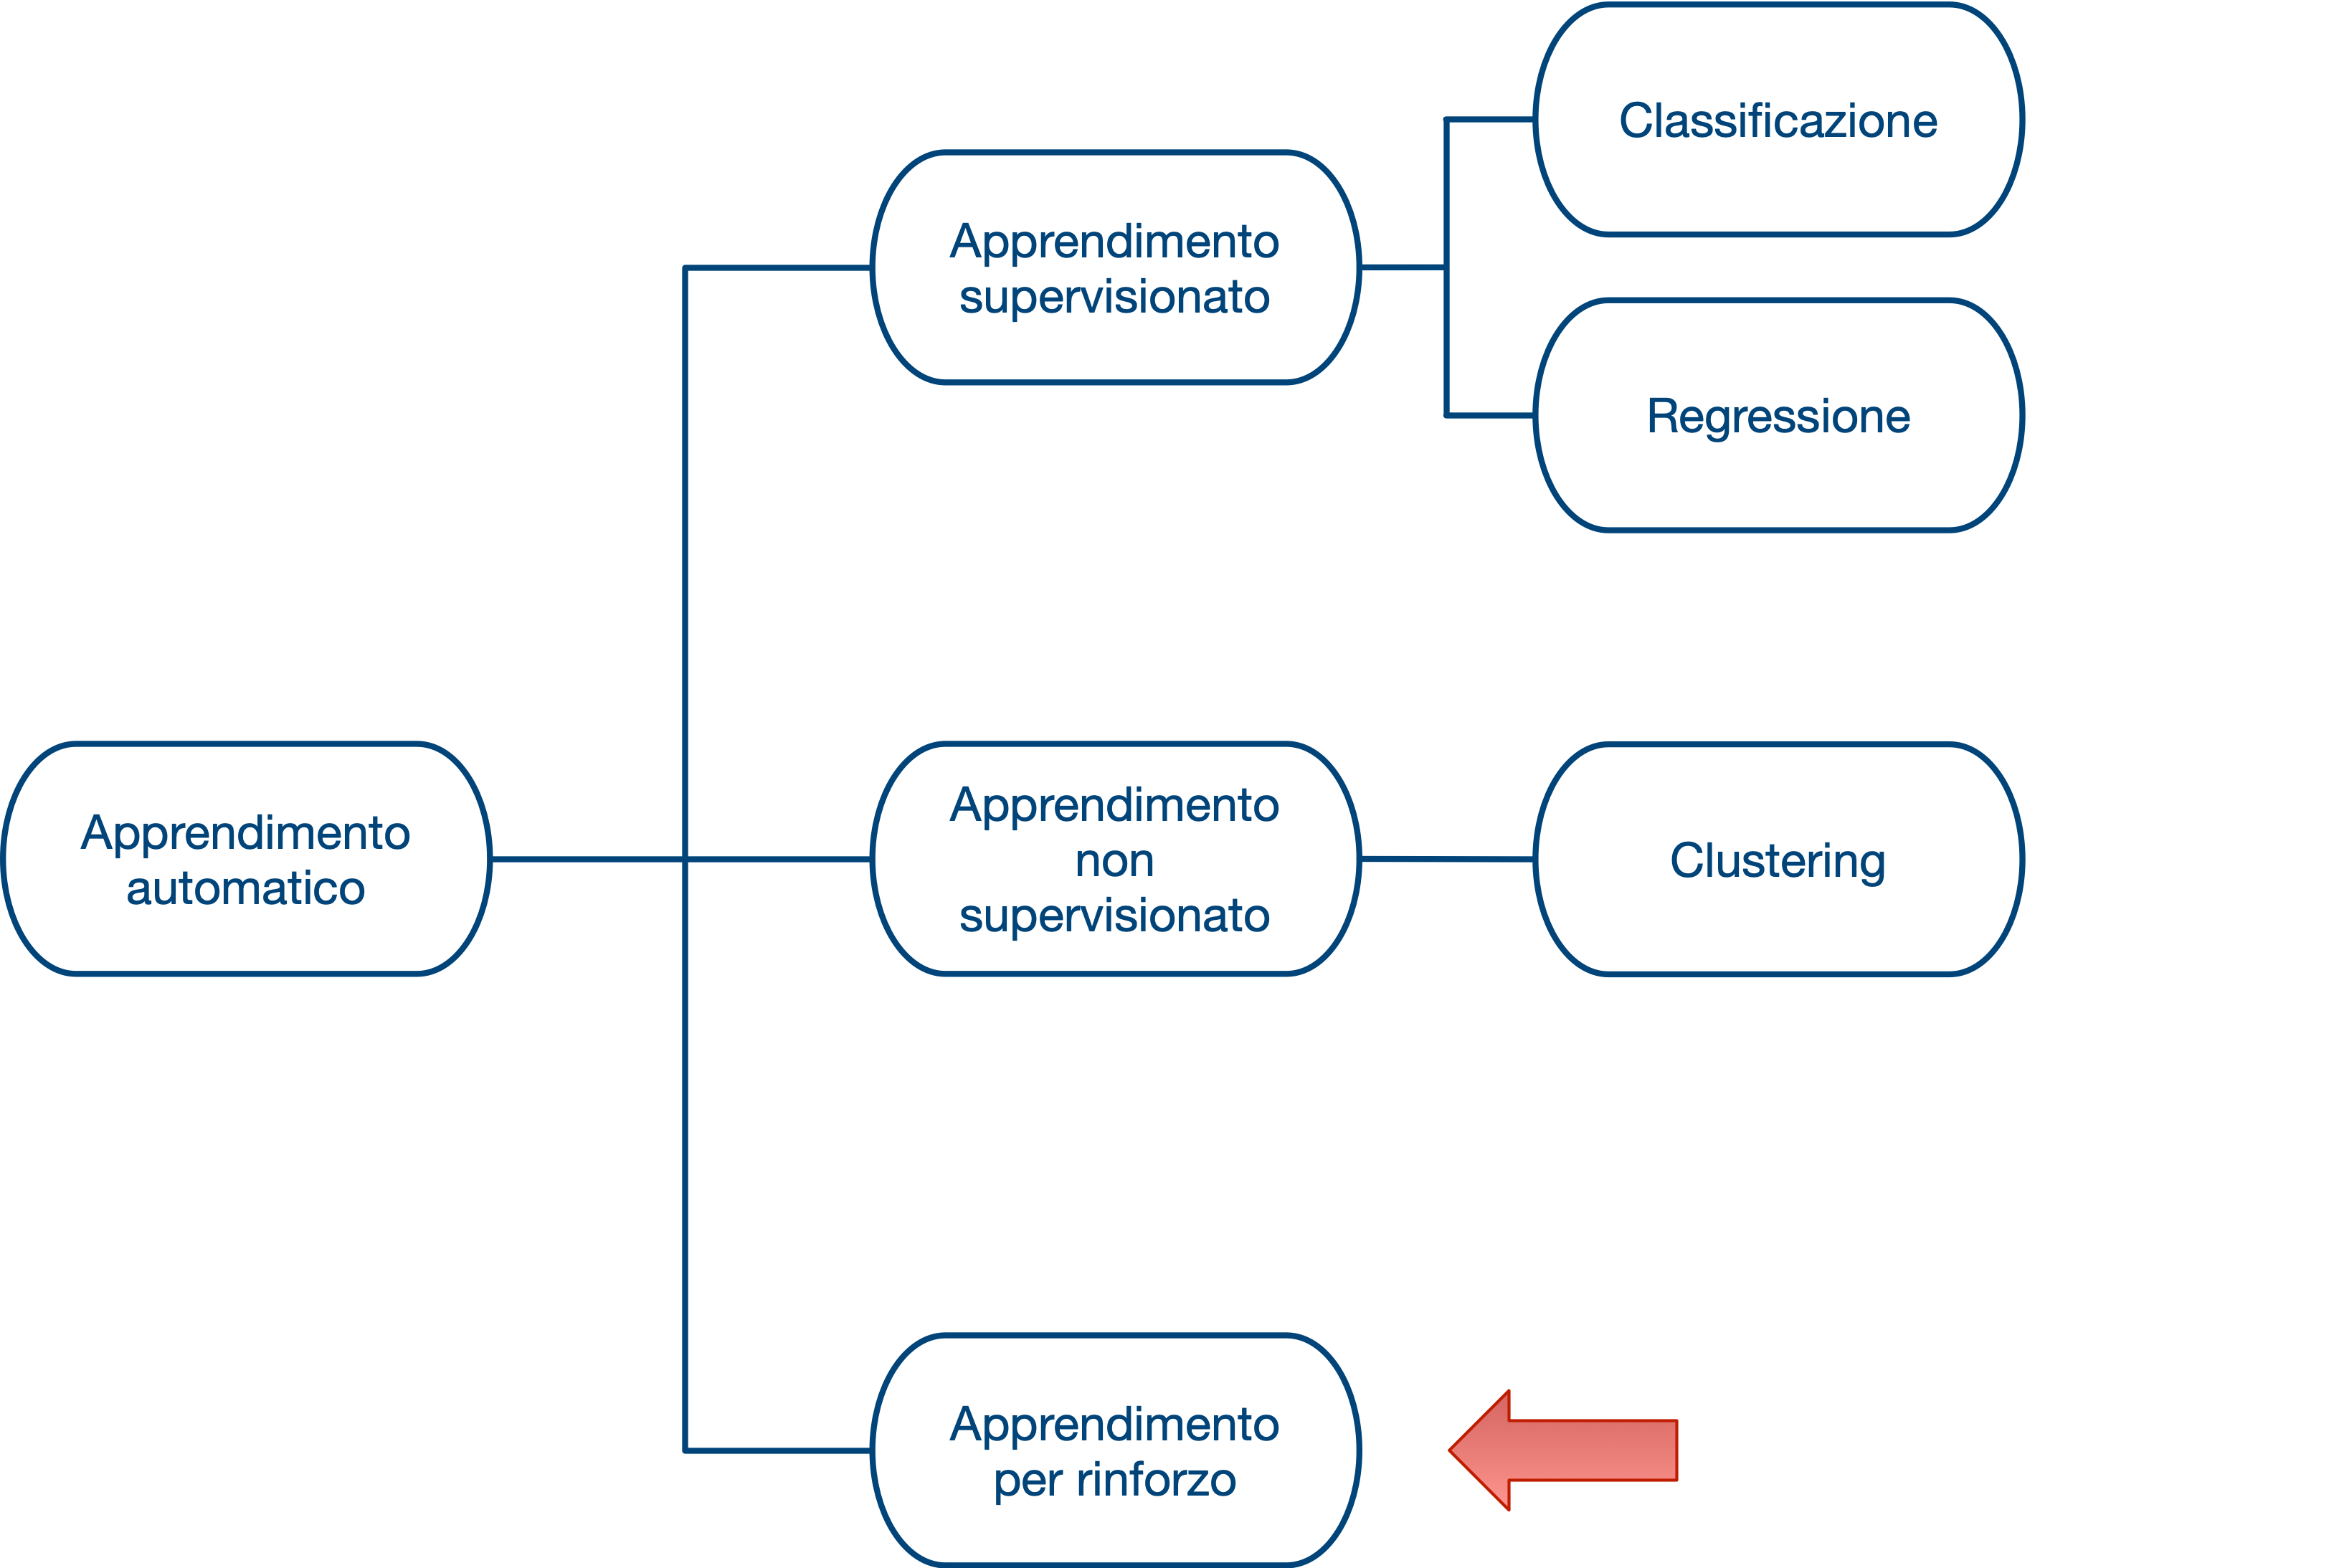
\includegraphics[scale=.2]{AAeASeANSeAPR.png}
    \end{center}
    \begin{flushright}
        {\tiny\textit{\textcopyright Simone Scannapieco}}
    \end{flushright}
    {\footnotesize
        \begin{itemize}[leftmargin=10pt,align=right]
            \item[\alert{\faArrowCircleRight}] Problemi di decisione sequenziali (decidere l'azione futura in base allo stato attuale)
            \item[\alert{\faArrowCircleRight}] Meccanismo interno che valuta l'efficacia dell'azione (rispetto a parametri)
            \begin{itemize}[leftmargin=10pt,align=right]
                \item[\alert{\faArrowCircleRight}] Azioni efficaci vengono \alert{premiate}
                \item[\alert{\faArrowCircleRight}] Azioni inefficaci vengono \alert{penalizzate}
            \end{itemize}\end{itemize}
    }
}
\only<7|handout:6>{
    \begin{center}
        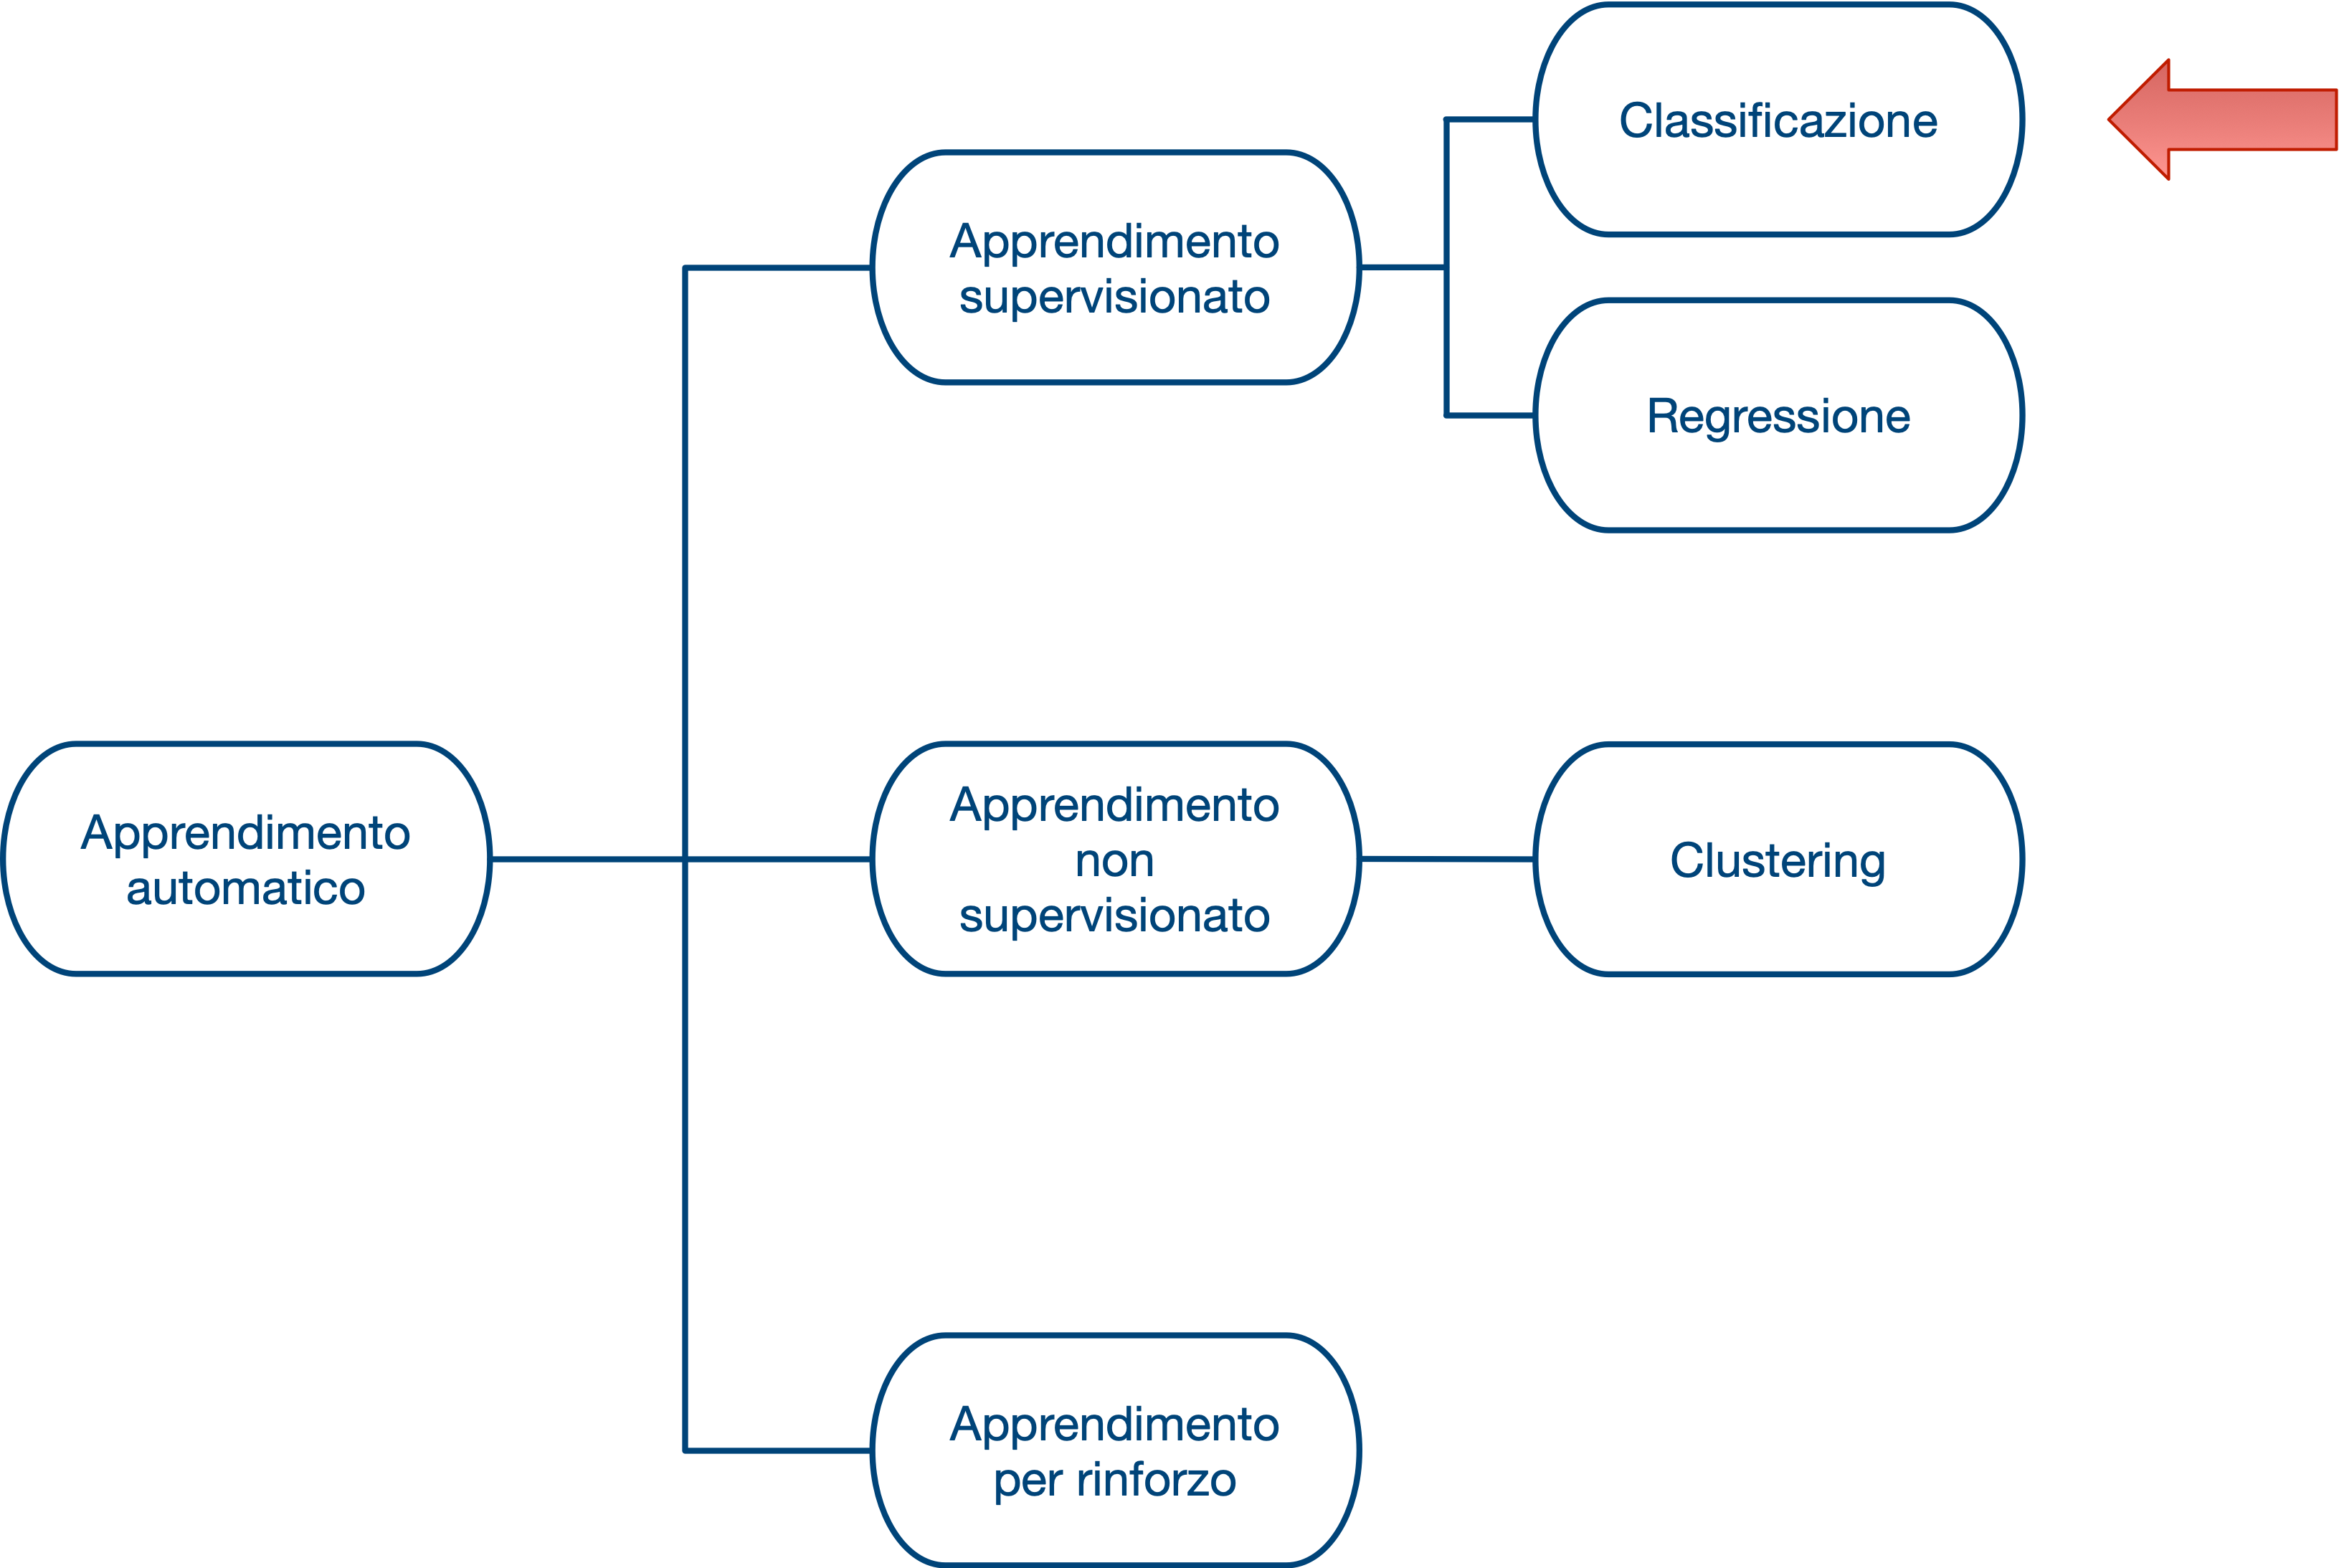
\includegraphics[scale=.2]{AAeASeANSeAPRConFrecciaSuClassificazione.png}
    \end{center}
    \begin{flushright}
        {\tiny\textit{\textcopyright Simone Scannapieco}}
    \end{flushright}
    {\footnotesize
        \begin{itemize}[leftmargin=10pt,align=right]
            \item[\alert{\faArrowCircleRight}] Ci concentriamo su \alert{addestramento supervisionato}
            \begin{itemize}[leftmargin=10pt,align=right]
                \item[\alert{\faArrowCircleRight}] Classificazione
                \item[\alert{\faArrowCircleRight}] Rilevamento entit\'{a} (caso speciale di classificazione)
            \end{itemize}
        \end{itemize}
    }
}
\end{frame}
%
\begin{frame}[t] \frametitle{Rappresentazione della conoscenza}
\framesubtitle{Cosa sono \emph{features} e parametri? Perché pre-processare?}
\begin{center}
    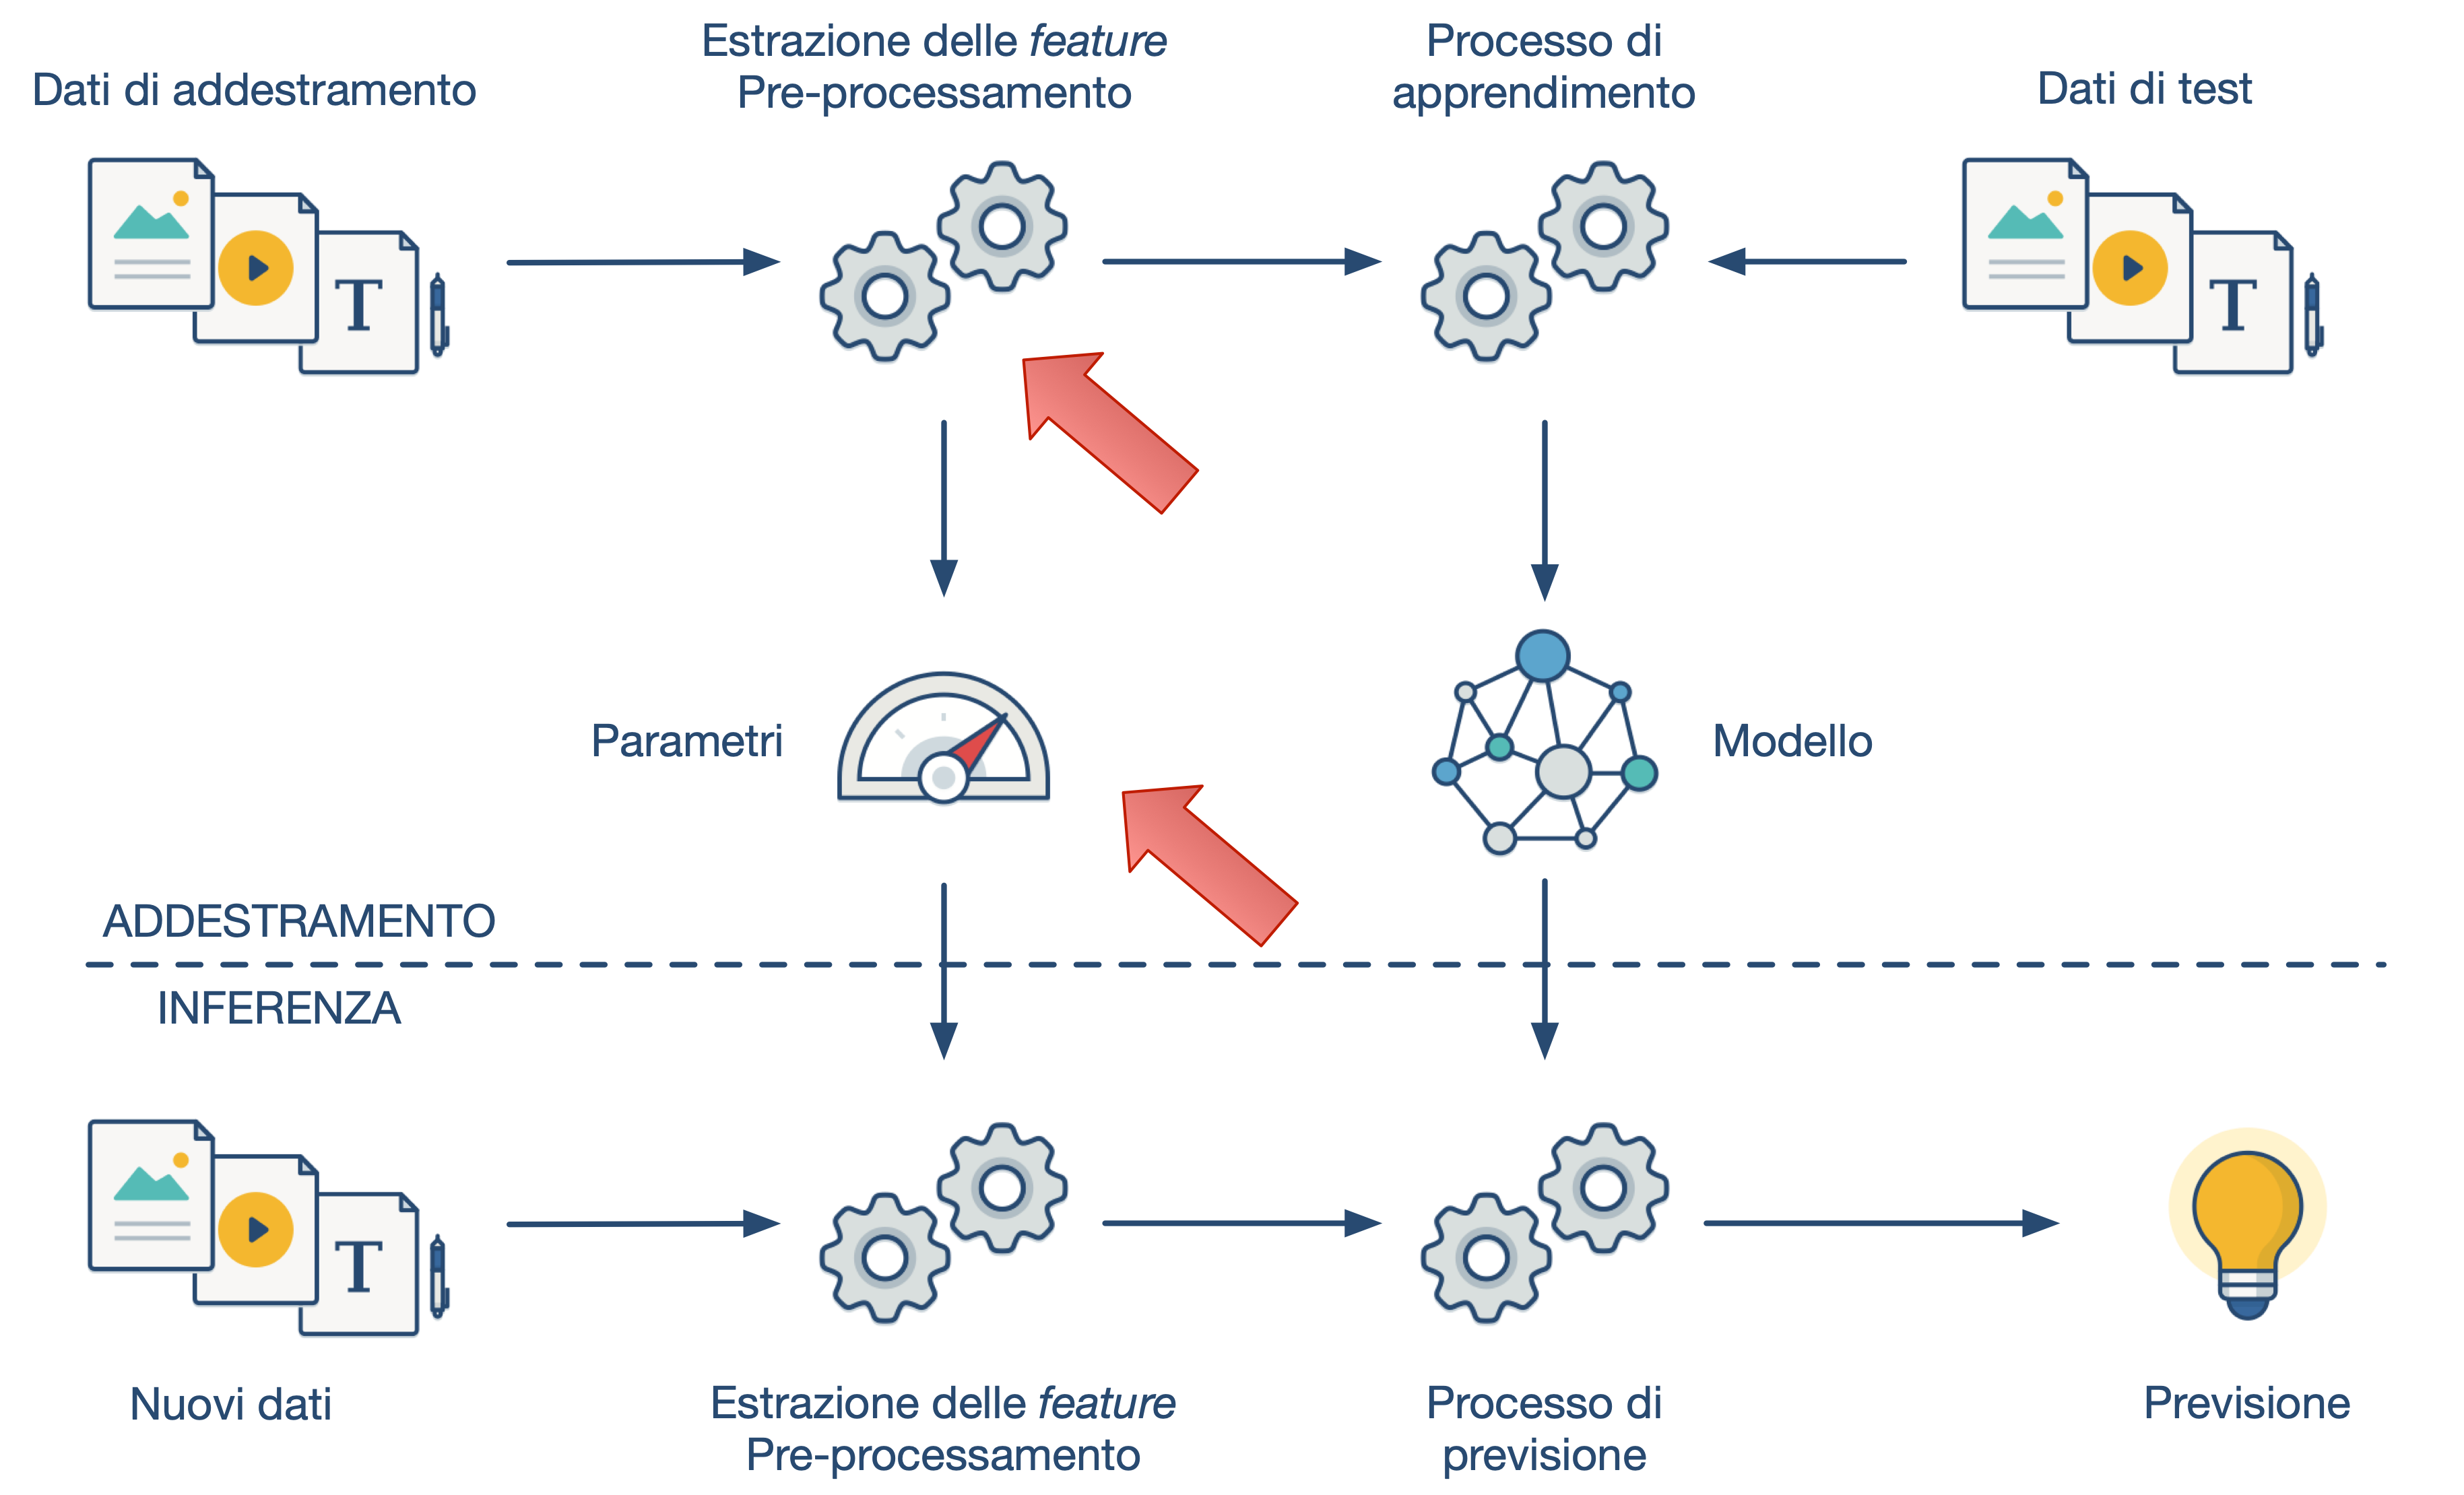
\includegraphics[height=6cm,keepaspectratio]{MLWithParametersAndArrowOnFEAndPAR.png}
\end{center}
\begin{flushright}
    {\tiny\textit{\textcopyright Simone Scannapieco}}
\end{flushright}
\end{frame}
%
\begin{frame}[t] \frametitle{Rappresentazione della conoscenza}
\framesubtitle{Estrazione delle \emph{features}}
\begin{center}
    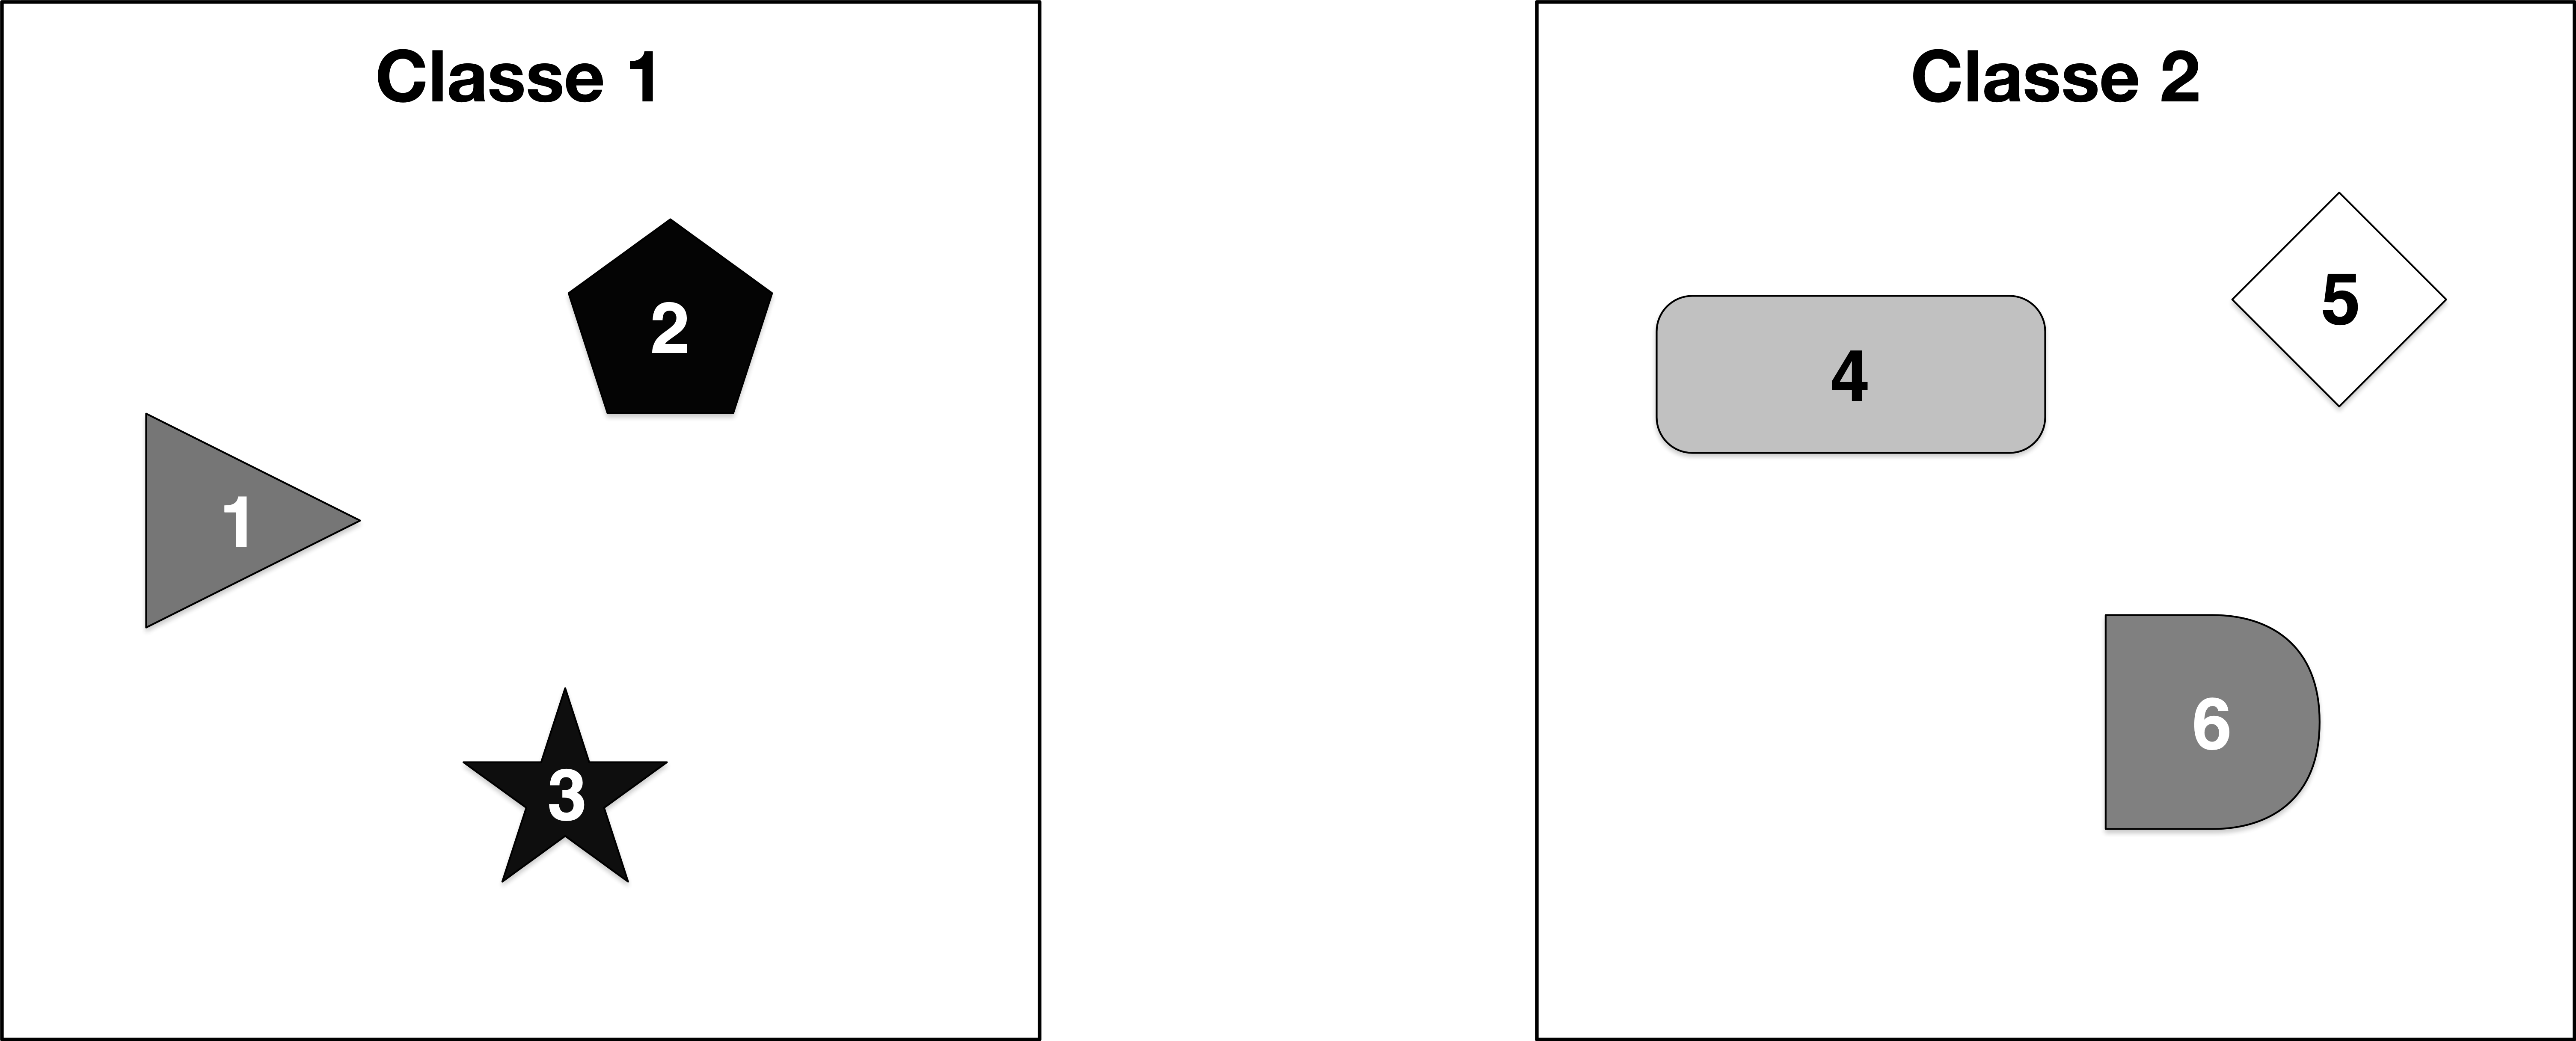
\includegraphics[scale=.09]{KRWithoutNewElements.png}
\end{center}
\only<1-4|handout:1>{
    \onslide<2-4>
    \begin{itemize}[leftmargin=10pt,align=right]
        \item[\alert{\faArrowCircleRight}] Come distinguere gli oggetti delle due classi?
        \onslide<3-4>
        \begin{itemize}[leftmargin=20pt,align=right]
            \item[\alert{\faArrowCircleRight}] Definire delle caratteristiche peculiari (\alert{\emph{features}})
            \onslide<4>
            \begin{itemize}[leftmargin=20pt,align=right]
                \item[\alert{\faArrowCircleRight}] Colore
                \item[\alert{\faArrowCircleRight}] Numero dei vertici
                \item[\alert{\faArrowCircleRight}] Forma dei vertici
            \end{itemize}
        \end{itemize}
    \end{itemize}
}
\only<5|handout:2>{
        {\scriptsize
    \begin{table}
        %% increase table row spacing, adjust to taste
        \renewcommand{\arraystretch}{1}
        \centering
        \begin{tabular}{crrrc}
            \toprule
            \textbf{Elemento} & \textbf{Colore} & \textbf{Vertici} & \textbf{Vertici arrotondati?} & \textbf{Classe}\\
            \midrule
            1 & Grigio medio  & 3  & No     & 1\\
            2 & Grigio scuro  & 5  & No     & 1\\
            3 & Grigio scuro  & 10 & No     & 1\\
            4 & Grigio chiaro & 4  & S\'{i} & 2\\
            5 & Bianco        & 4  & No     & 2\\
            6 & Grigio medio  & 4  & S\'{i} & 2\\
            \bottomrule
        \end{tabular}
    \end{table}
    }
}
\only<6-8|handout:3>{
    \onslide<6-8>
    \begin{itemize}[leftmargin=10pt,align=right]
        \item[\alert{\faArrowCircleRight}] Il linguaggio macchina \'{e} \alert{numerico}
        \onslide<7-8>
        \begin{itemize}[leftmargin=20pt,align=right]
            \item[\alert{\faArrowCircleRight}] Tradurre i valori delle \emph{features}
            \onslide<8>
            \begin{itemize}[leftmargin=20pt,align=right]
                \item[\alert{\faArrowCircleRight}] Colore: intero in \alert{$[0,255]$} (0 = nero, 255 = bianco)
                \item[\alert{\faArrowCircleRight}] Numero dei vertici: intero in \alert{$[3,n]$} ($n$ fissato a priori)
                \item[\alert{\faArrowCircleRight}] Forma dei vertici: booleano in \alert{$[0,1]$} (0 = No, 1 = S\'{i})
            \end{itemize}
        \end{itemize}
    \end{itemize}
}
\only<9|handout:4>{
        {\scriptsize
    \begin{table}
        %% increase table row spacing, adjust to taste
        \renewcommand{\arraystretch}{1}
        \centering
        \begin{tabular}{crrrcr}
            \toprule
            \textbf{Elemento} & \textbf{Colore} & \textbf{Vertici} & \textbf{Vertici arrotondati?} & \textbf{Classe} & \textbf{\emph{Feature vector}}\\
            \midrule
            1 & 120 & 3  & 0 & 1 & $[120,3,0]$\\
            2 & 5   & 5  & 0 & 1 & $[5,5,0]$\\
            3 & 10  & 10 & 0 & 1 & $[10,10,0]$\\
            4 & 196 & 4  & 1 & 2 & $[196,4,1]$\\
            5 & 255 & 4  & 0 & 2 & $[255,4,0]$\\
            6 & 128 & 4  & 1 & 2 & $[128,4,1]$\\
            \bottomrule
        \end{tabular}
    \end{table}
    }
}
\end{frame}
%
\begin{frame}[t] \frametitle{Rappresentazione della conoscenza}
\framesubtitle{Perch\'{e} pre-processare i dati?}
\only<1|handout:0>{
    \begin{center}
        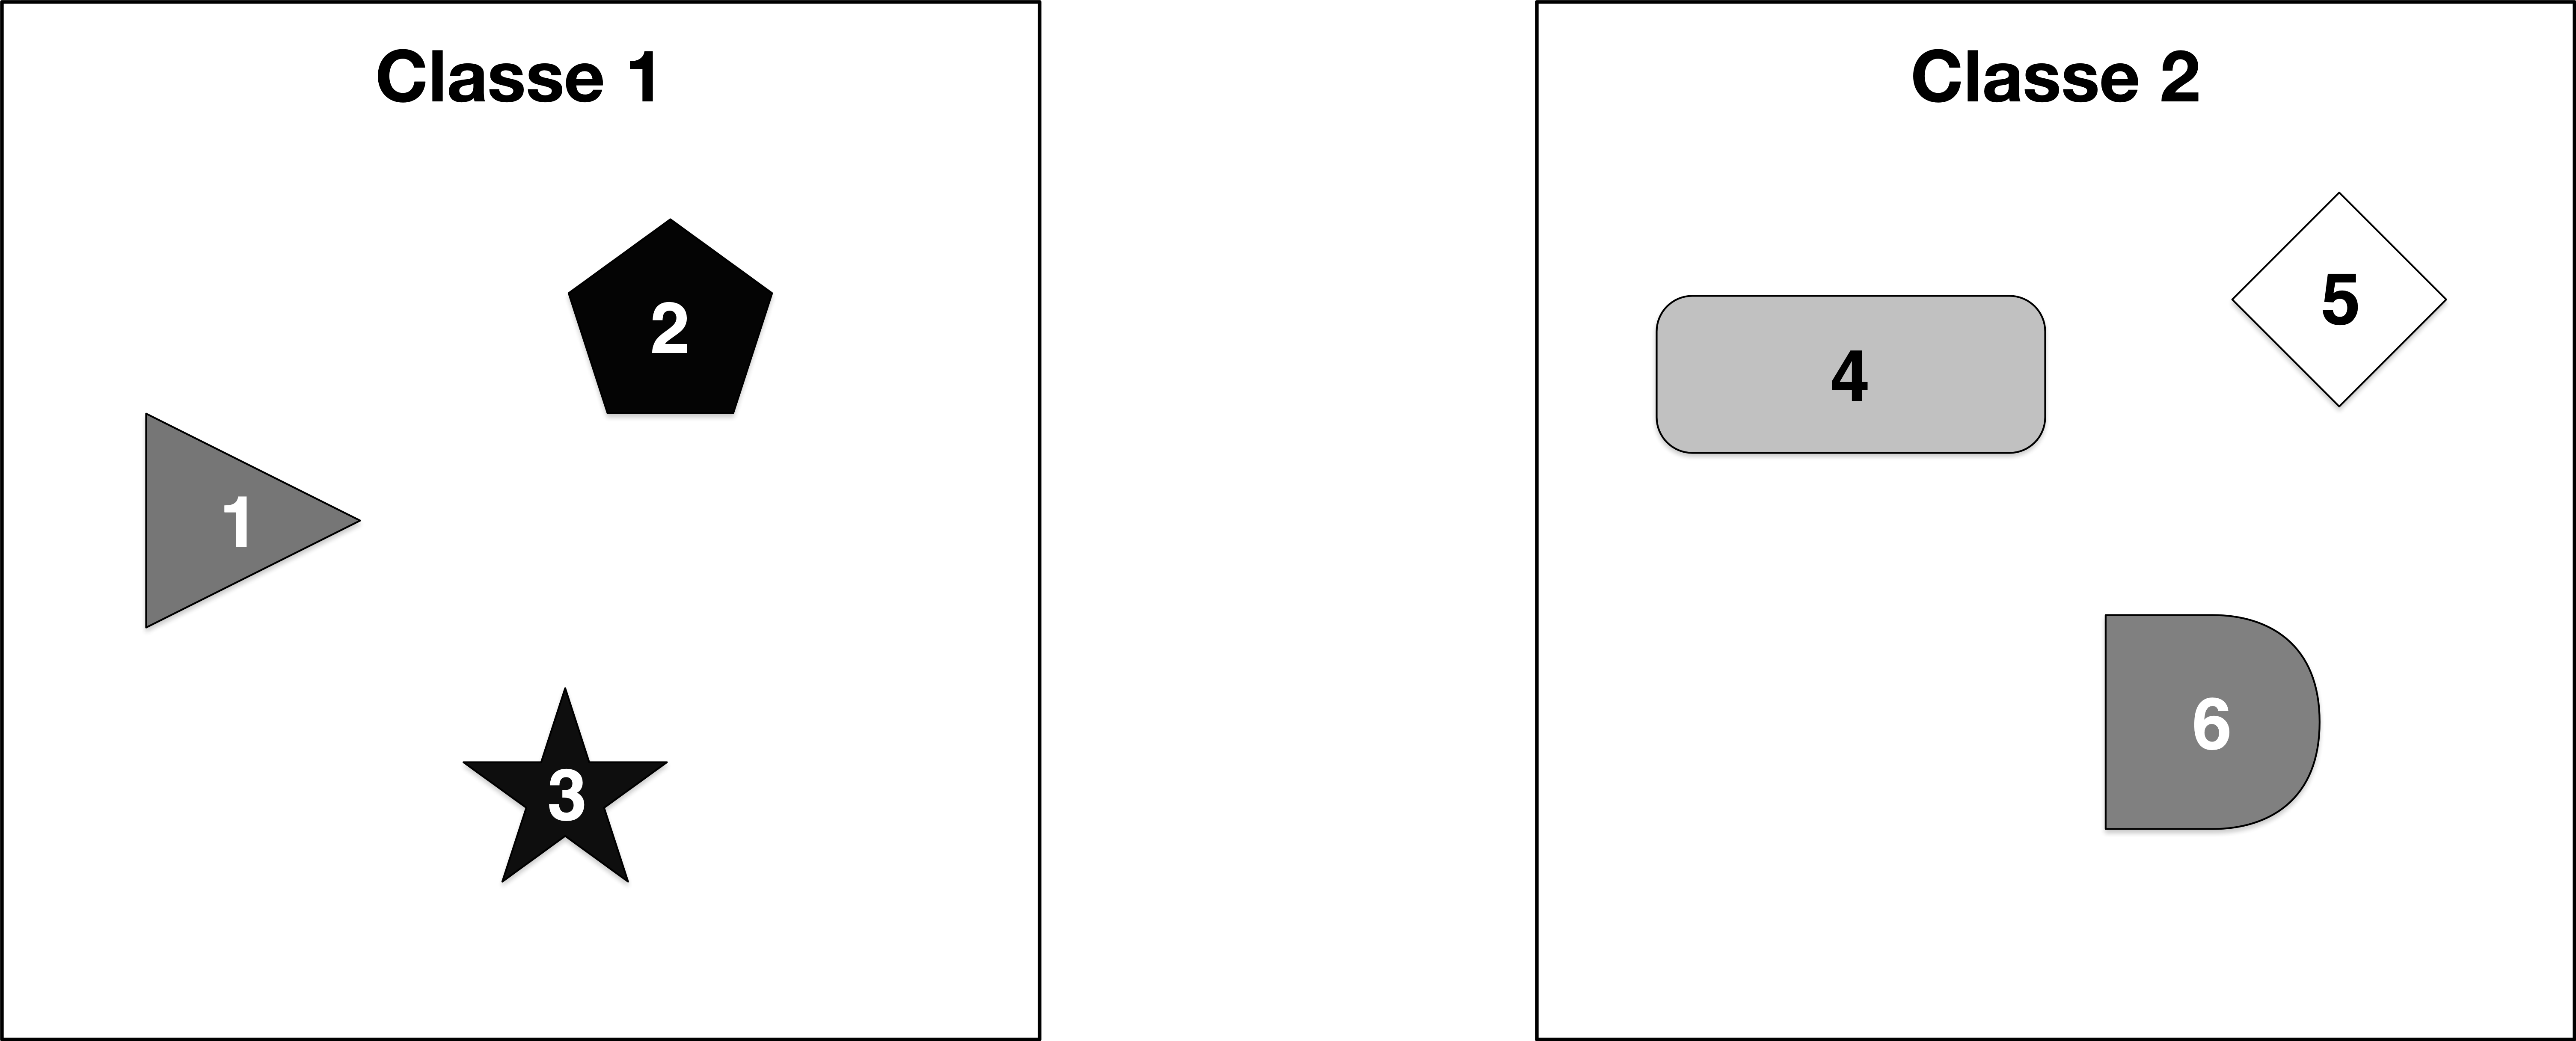
\includegraphics[scale=.09]{KRWithoutNewElements.png}
    \end{center}
}
\only<2-4|handout:1>{
    \begin{center}
        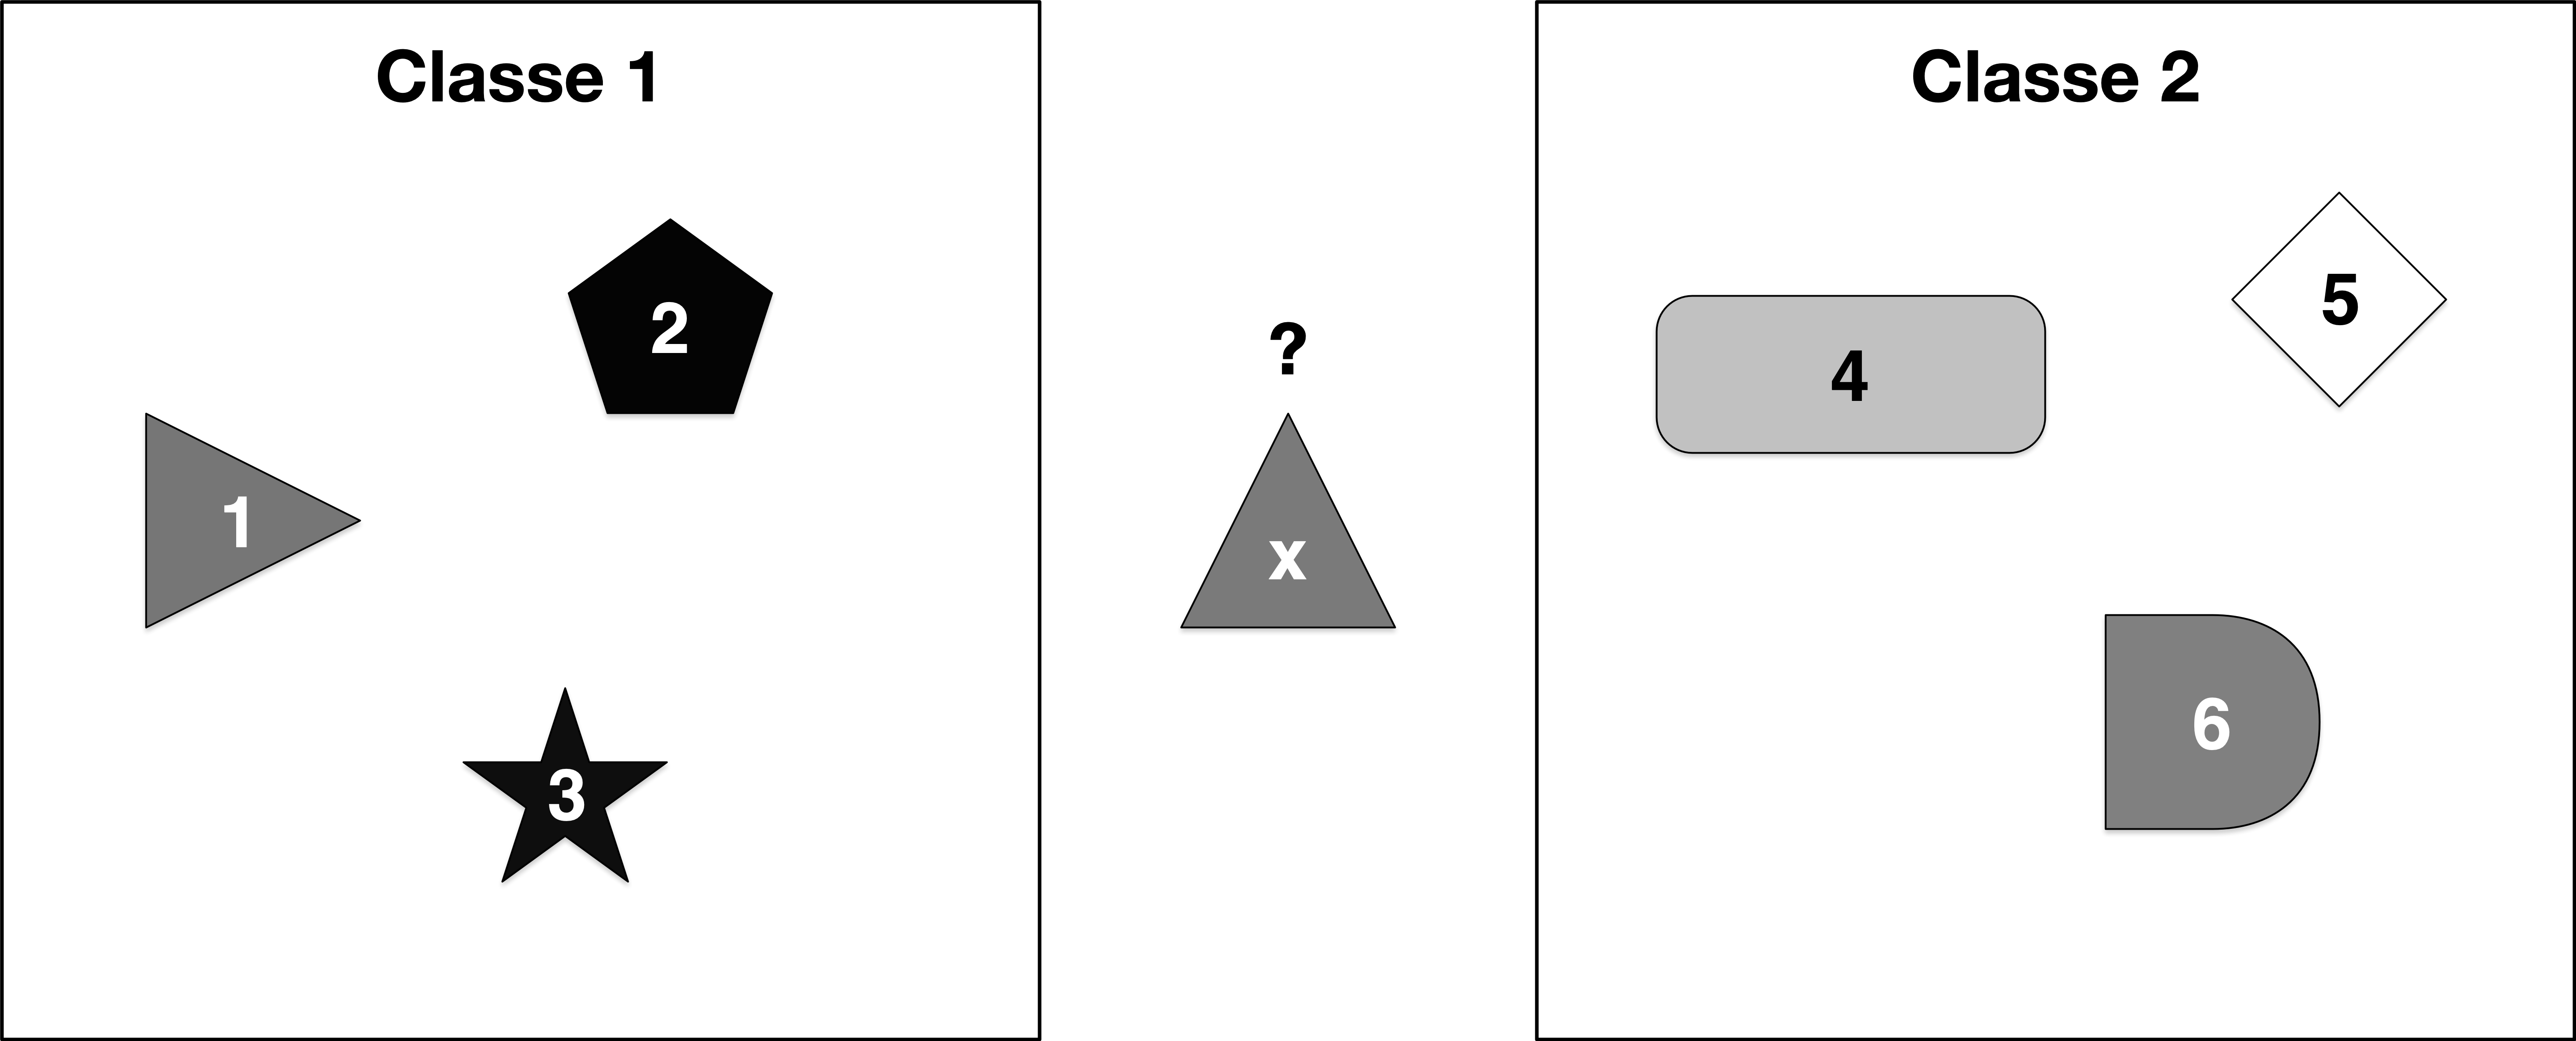
\includegraphics[scale=.09]{KRWithNewElementX.png}
    \end{center}
    \onslide<3-4>
    \begin{itemize}[leftmargin=10pt,align=right]
        \item[\alert{\faArrowCircleRight}] Esempio di algoritmo di classificazione\\
        {\scriptsize
            \begin{algorithm2e}[H]
                \SetAlgoLined
                \KwData{Un nuovo elemento \emph{x}}
                \KwResult{La classe \emph{C} di appartenenza di \emph{x}}
                \For{elemento y in \set{Classe 1, Classe 2}}{
                    Calcola la distanza \emph{d} fra \emph{y} ed \emph{x}\;
                }
                \emph{C} = classe dell'elemento \emph{y} che minimizza \emph{d}\;
            \end{algorithm2e}
        }
        \onslide<4>
        \item[\alert{\faArrowCircleRight}] Distanza intesa come \alert{euclidea} $d(y,x) = \sqrt{\sum_{i=1}^{n}(y_{i} - x_{i})^{2}}$
    \end{itemize}
}
\only<5-7|handout:2>{
    \begin{center}
        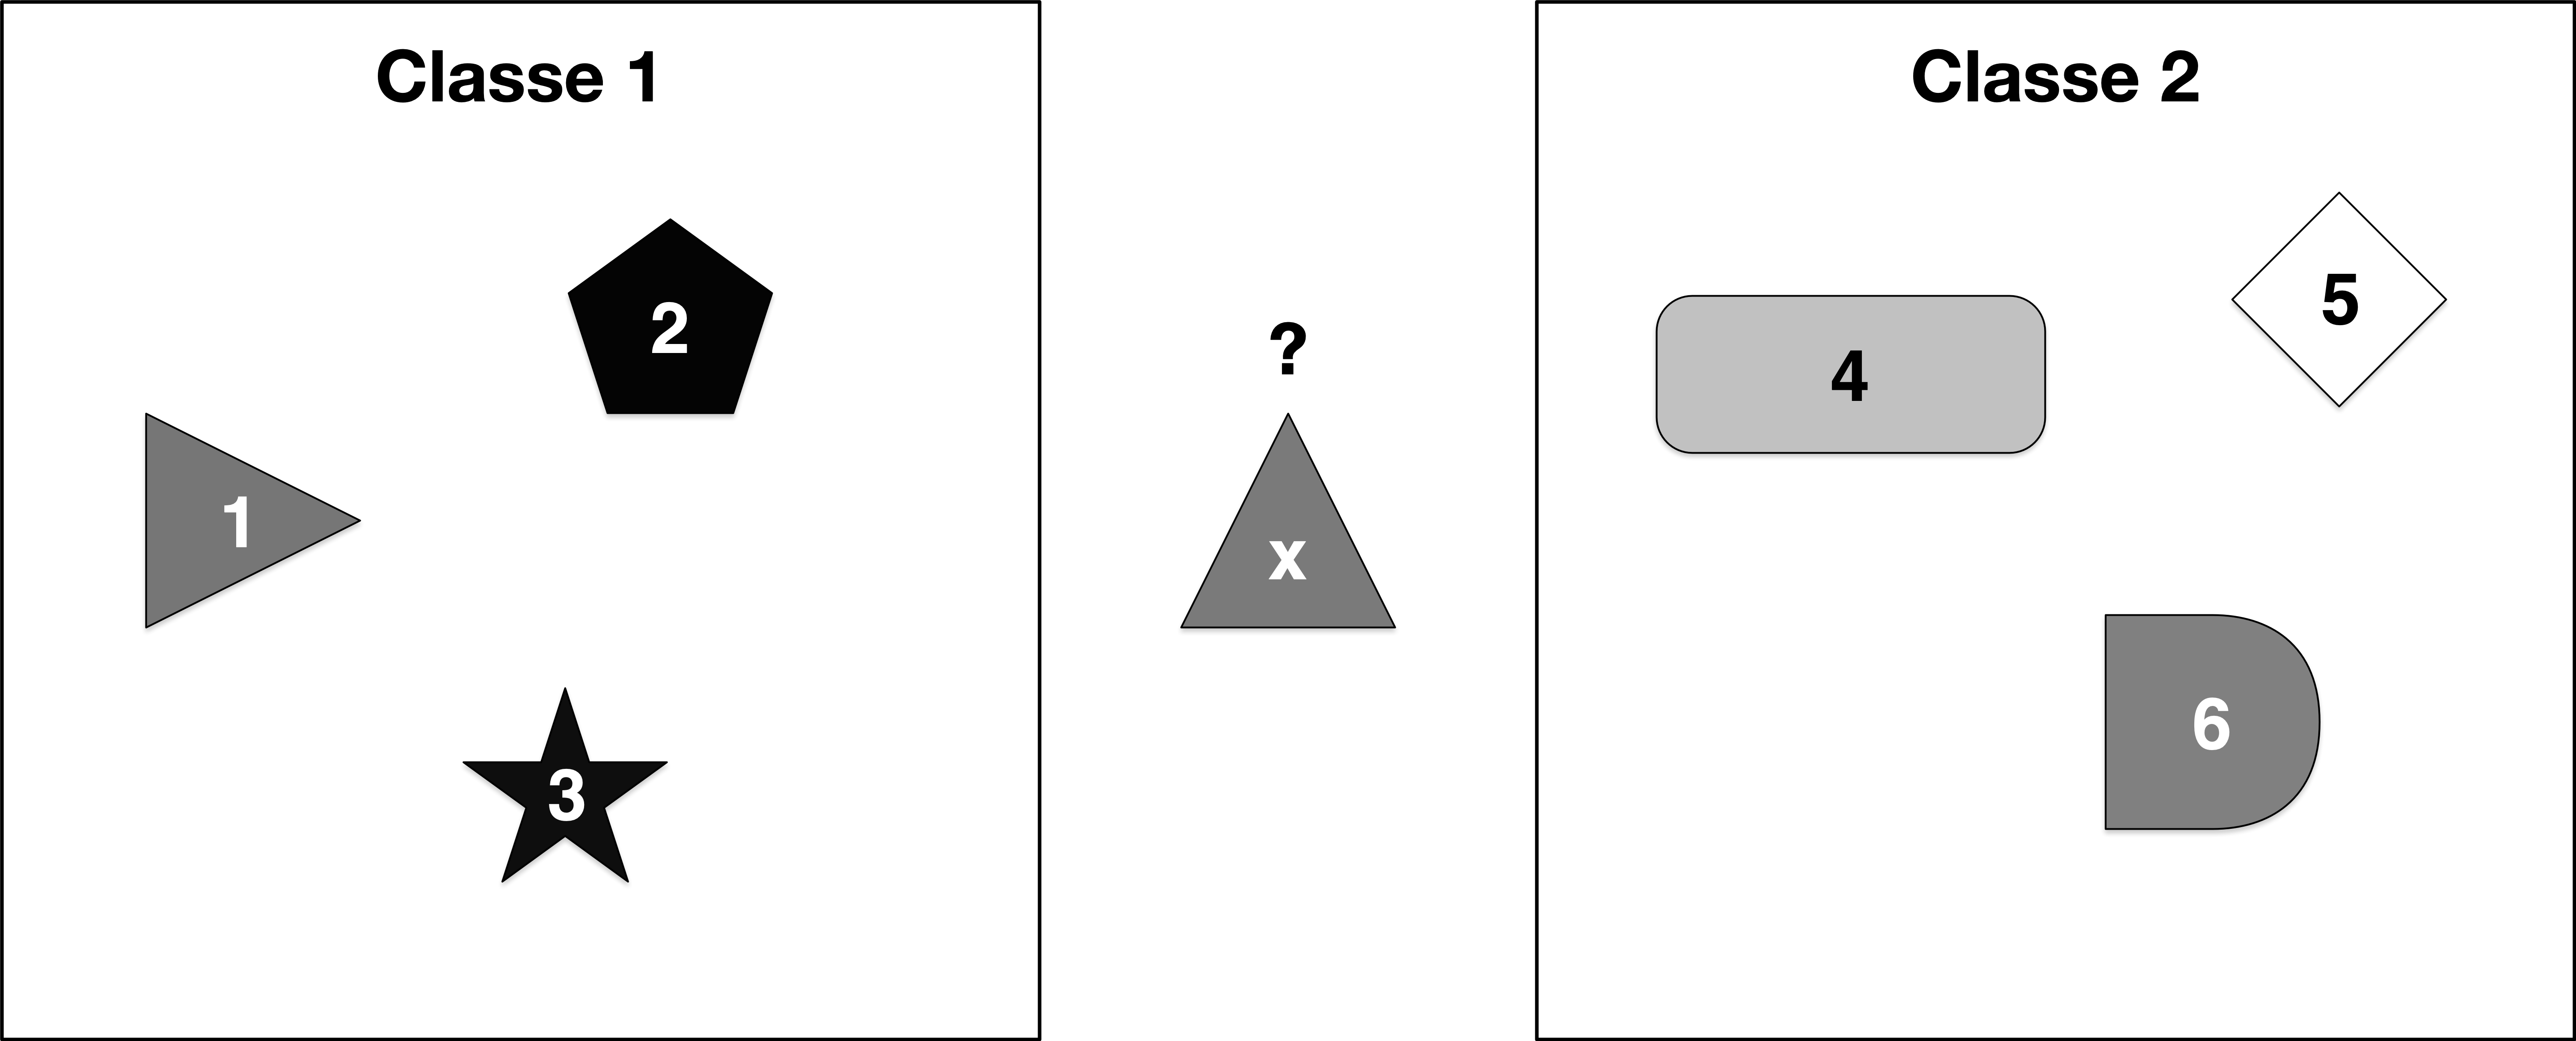
\includegraphics[scale=.09]{KRWithNewElementX.png}
    \end{center}
    \onslide<5-7>
    {\scriptsize
        \begin{itemize}[leftmargin=10pt,align=right]
            \item[\alert{\faArrowCircleRight}] Con x = $[123,3,0]$\\
            \onslide<6-7>
            %
            \[
                \begin{rcases*}
                    d(1,x) = \sqrt{(-3)^{2} + 0^{2} + 0^{2}} = \alert{\mathbf{3}} \\
                    d(2,x) = \sqrt{(-118)^{2} + 2^{2} + 0^{2}} = 118.01 \\
                    d(3,x) = \sqrt{(-113)^{2} + 7^{2} + 0^{2}} = 113.21 \\
                    d(4,x) = \sqrt{73^{2} + 1^{2} + 1^{2}} = 73.01 \\
                    d(5,x) = \sqrt{132^{2} + 1^{2} + 0^{2}} = 132.003 \\
                    d(6,x) = \sqrt{5^{2} + 1^{2} + 1^{2}} = 5.19
                \end{rcases*} C = 1 \onslide<7> \quad\text{ \alert{\faHandOLeft\ \textbf{Previsione plausibile}}}
            \]
        \end{itemize}
    }
}
\only<8-10|handout:3>{
    \begin{center}
        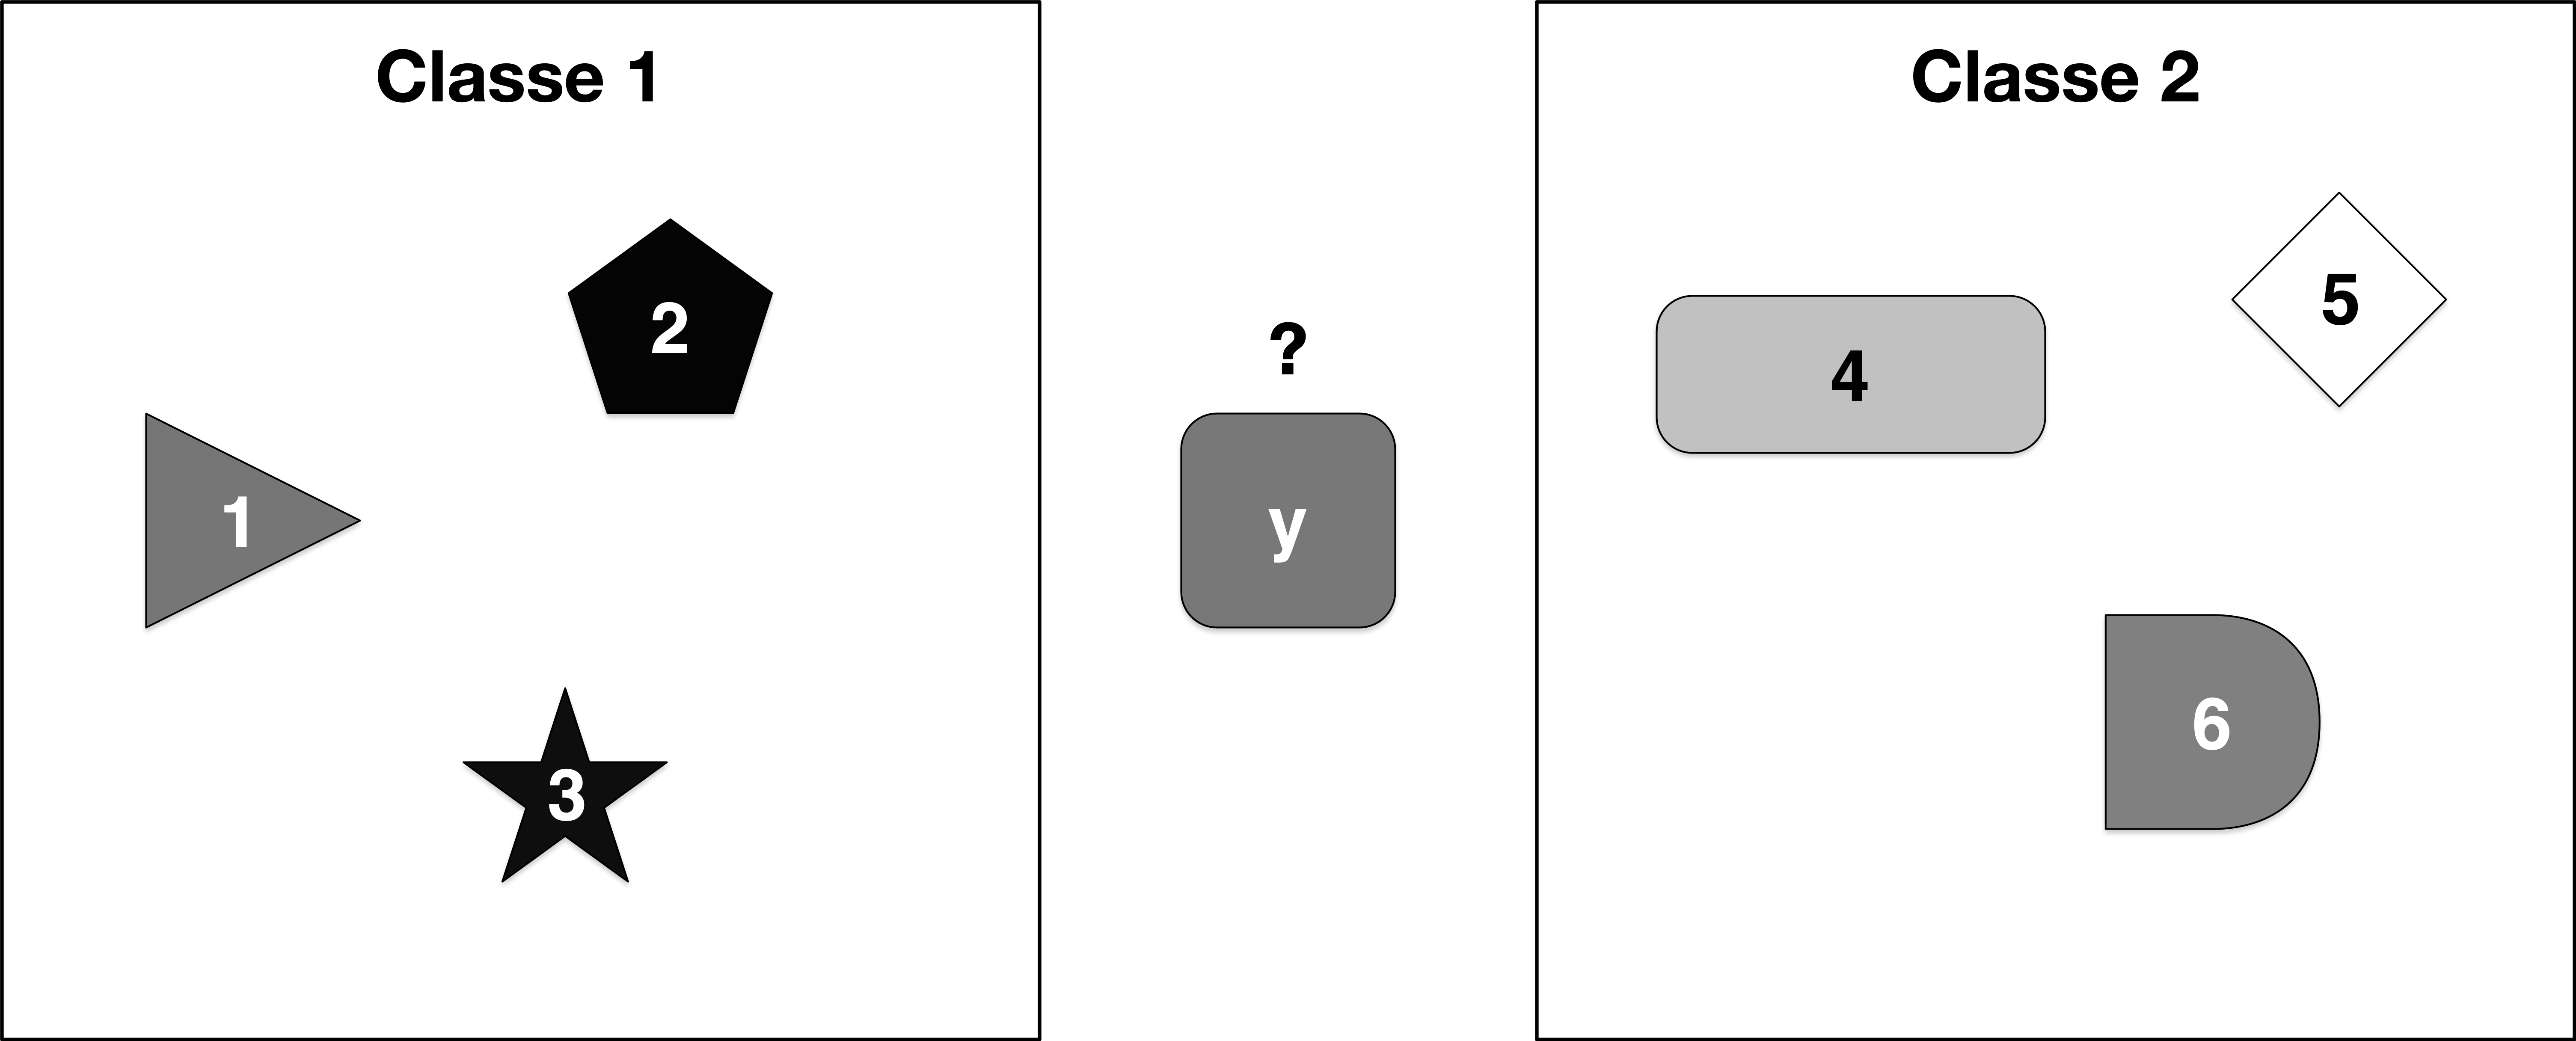
\includegraphics[scale=.09]{KRWithNewElementY.png}
    \end{center}
    \onslide<8-10>
    {\scriptsize
        \begin{itemize}[leftmargin=10pt,align=right]
            \item[\alert{\faArrowCircleRight}] Con y = $[120,4,1]$\\
            \onslide<9-10>
            %
            \[
                \begin{rcases*}
                    d(1,y) = \sqrt{0^{2} + (-1)^{2} + (-1)^{2}} = \alert{\mathbf{1.41}} \\
                    d(2,y) = \sqrt{(-115)^{2} + 1^{2} + (-1)^{2}} = 115.008 \\
                    d(3,y) = \sqrt{(-110)^{2} + 6^{2} + (-1)^{2}} = 110.16 \\
                    d(4,y) = \sqrt{76^{2} + 0^{2} + 0^{2}} = 73.01 \\
                    d(5,y) = \sqrt{135^{2} + 0^{2} + (-1)^{2}} = 135.003 \\
                    d(6,y) = \sqrt{8^{2} + 0^{2} + 0^{2}} = 8
                \end{rcases*} C = 1 \onslide<10> \quad\text{\color{red}{\faHandOLeft\ \textbf{Previsione non plausibile}}}
            \]
        \end{itemize}
    }
}
\only<11-12|handout:4>{
    \begin{center}
        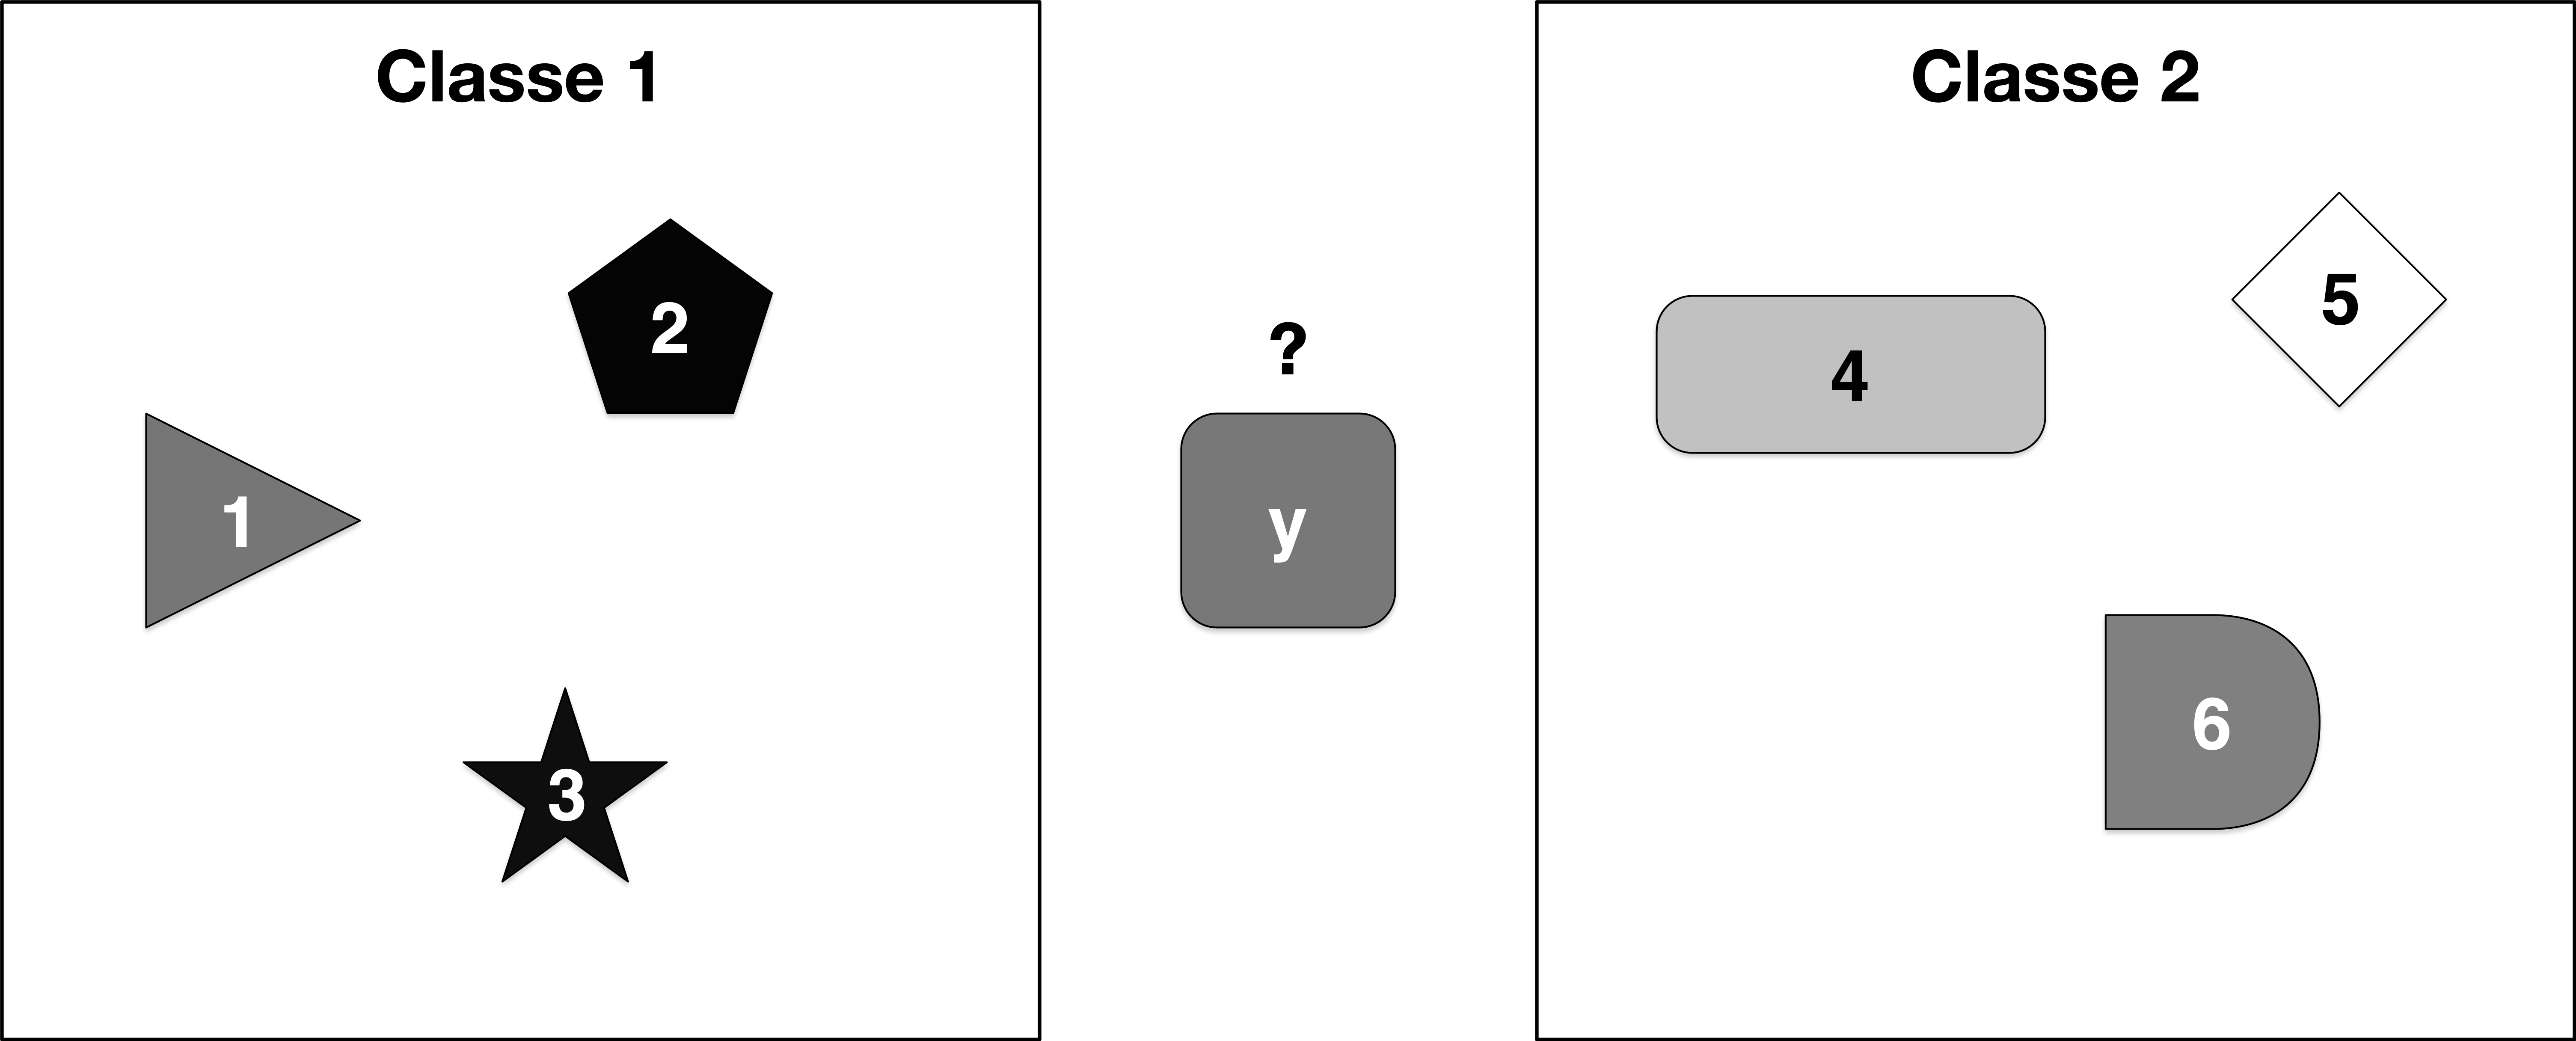
\includegraphics[scale=.09]{KRWithNewElementY.png}
    \end{center}
    \onslide<11-12>
    {\scriptsize
        \begin{itemize}[leftmargin=10pt,align=right]
            \item[\alert{\faArrowCircleRight}] La \emph{feature} colore maschera le altre due\\
            \onslide<12>
            %
            \[
                \begin{rcases*}
                    d(1,y) = \sqrt{0^{2} + (-1)^{2} + (-1)^{2}} = 1.41 \\
                    d(2,y) = \sqrt{(-\begingroup\color{red}\mathbf{115}\endgroup)^{2} + 1^{2} + (-1)^{2}} = \begingroup\color{red}\mathbf{115.008}\endgroup \\
                    d(3,y) = \sqrt{(-\begingroup\color{red}\mathbf{110}\endgroup)^{2} + 6^{2} + (-1)^{2}} = \begingroup\color{red}\mathbf{110.16}\endgroup \\
                    d(4,y) = \sqrt{\begingroup\color{red}\mathbf{76}\endgroup^{2} + 0^{2} + 0^{2}} = \begingroup\color{red}\mathbf{73.01}\endgroup \\
                    d(5,y) = \sqrt{\begingroup\color{red}\mathbf{135}\endgroup^{2} + 0^{2} + (-1)^{2}} = \begingroup\color{red}\mathbf{135.003}\endgroup \\
                    d(6,y) = \sqrt{\begingroup\color{red}\mathbf{8}\endgroup^{2} + 0^{2} + 0^{2}} = \begingroup\color{red}\mathbf{8}\endgroup
                \end{rcases*} \color{red}{d(n,y) \approx y_{1}}
            \]
        \end{itemize}
    }
}
\only<13-14|handout:5>{
    \begin{center}
        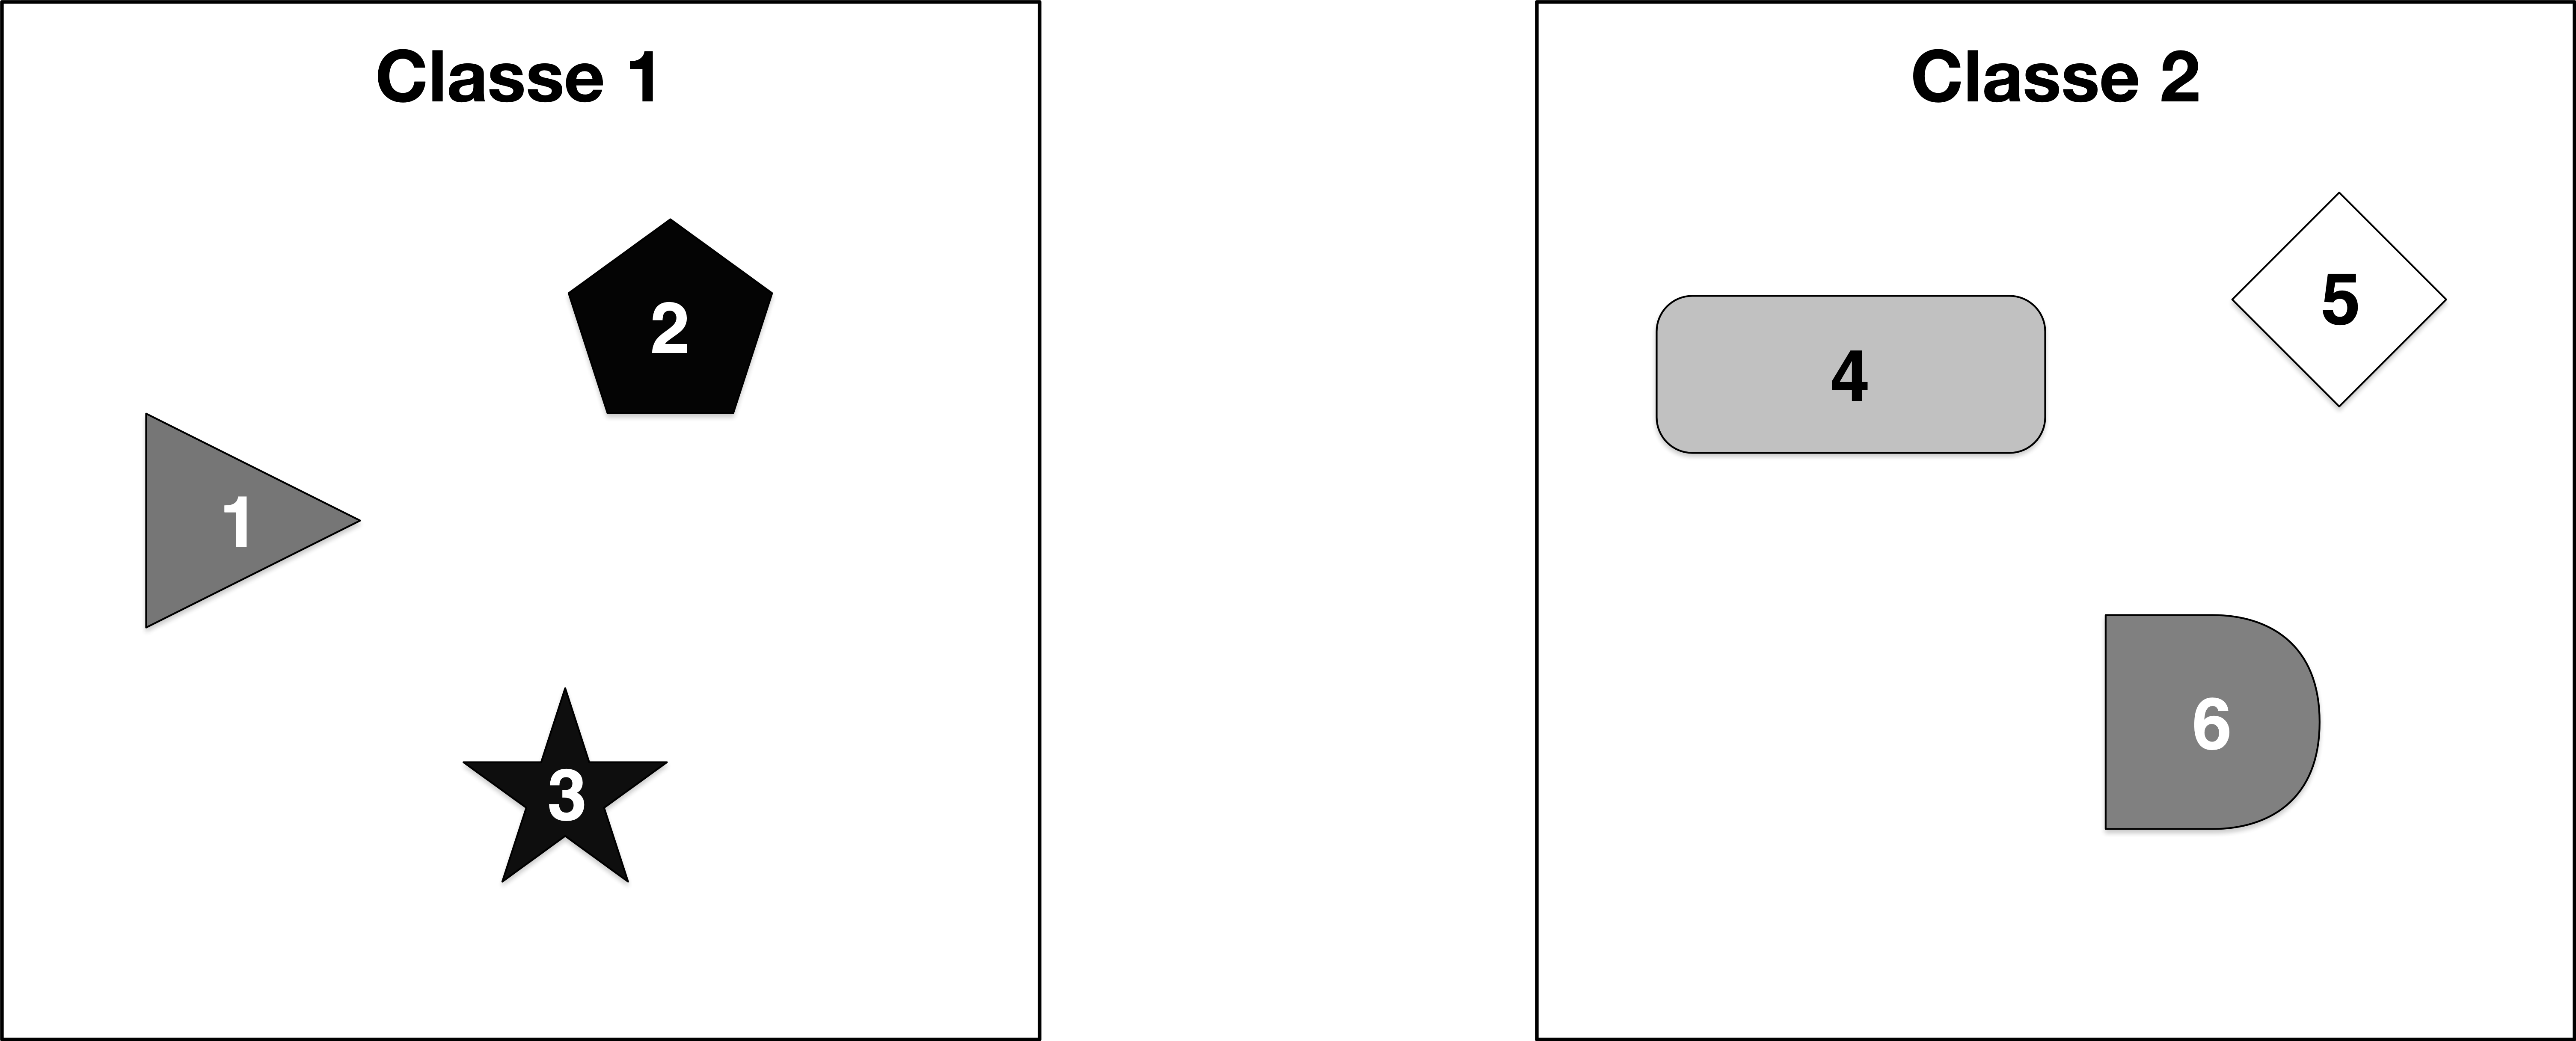
\includegraphics[scale=.09]{KRWithoutNewElements.png}
    \end{center}
    \onslide<13-14>
    {\scriptsize
        \begin{itemize}[leftmargin=10pt,align=right]
            \item[\alert{\faArrowCircleRight}] Necessaria \alert{normalizzazione} per rendere paragonabili tutte le \emph{features} $\Big($es. $\overline{n_{i}} = \frac{n_{i}-n_{min}}{n_{max}-n_{min}}\Big)$
            \item[\alert{\faArrowCircleRight}] Per colore ($n_{min}=0, n_{max} = 255$), per numero vertici ($n_{min} = 3, n_{max} = 10$)
            \onslide<14>
            {
            \begin{table}
                %% increase table row spacing, adjust to taste
                \renewcommand{\arraystretch}{1}
                \centering
                \begin{tabular}{crr}
                    \toprule
                    \textbf{Elemento} & \textbf{\emph{Feature vector}} & \textbf{Normalizzazione}\\
                    \midrule
                    1 & $[120,3,0]$ & $[0.47,0,0]$\\
                    2 & $[5,5,0]$ & $[0.01,0.28,0]$\\
                    3 & $[10,10,0]$ & $[0.03,1,0]$\\
                    4 & $[196,4,1]$ & $[0.76,0.14,0]$\\
                    5 & $[255,4,0]$ & $[1,0.14,0]$\\
                    6 & $[128,4,1]$ & $[0.5,0.14,1]$\\
                    \bottomrule
                \end{tabular}
            \end{table}
            }
        \end{itemize}
    }
}
\only<15-16|handout:6>{
    \begin{center}
        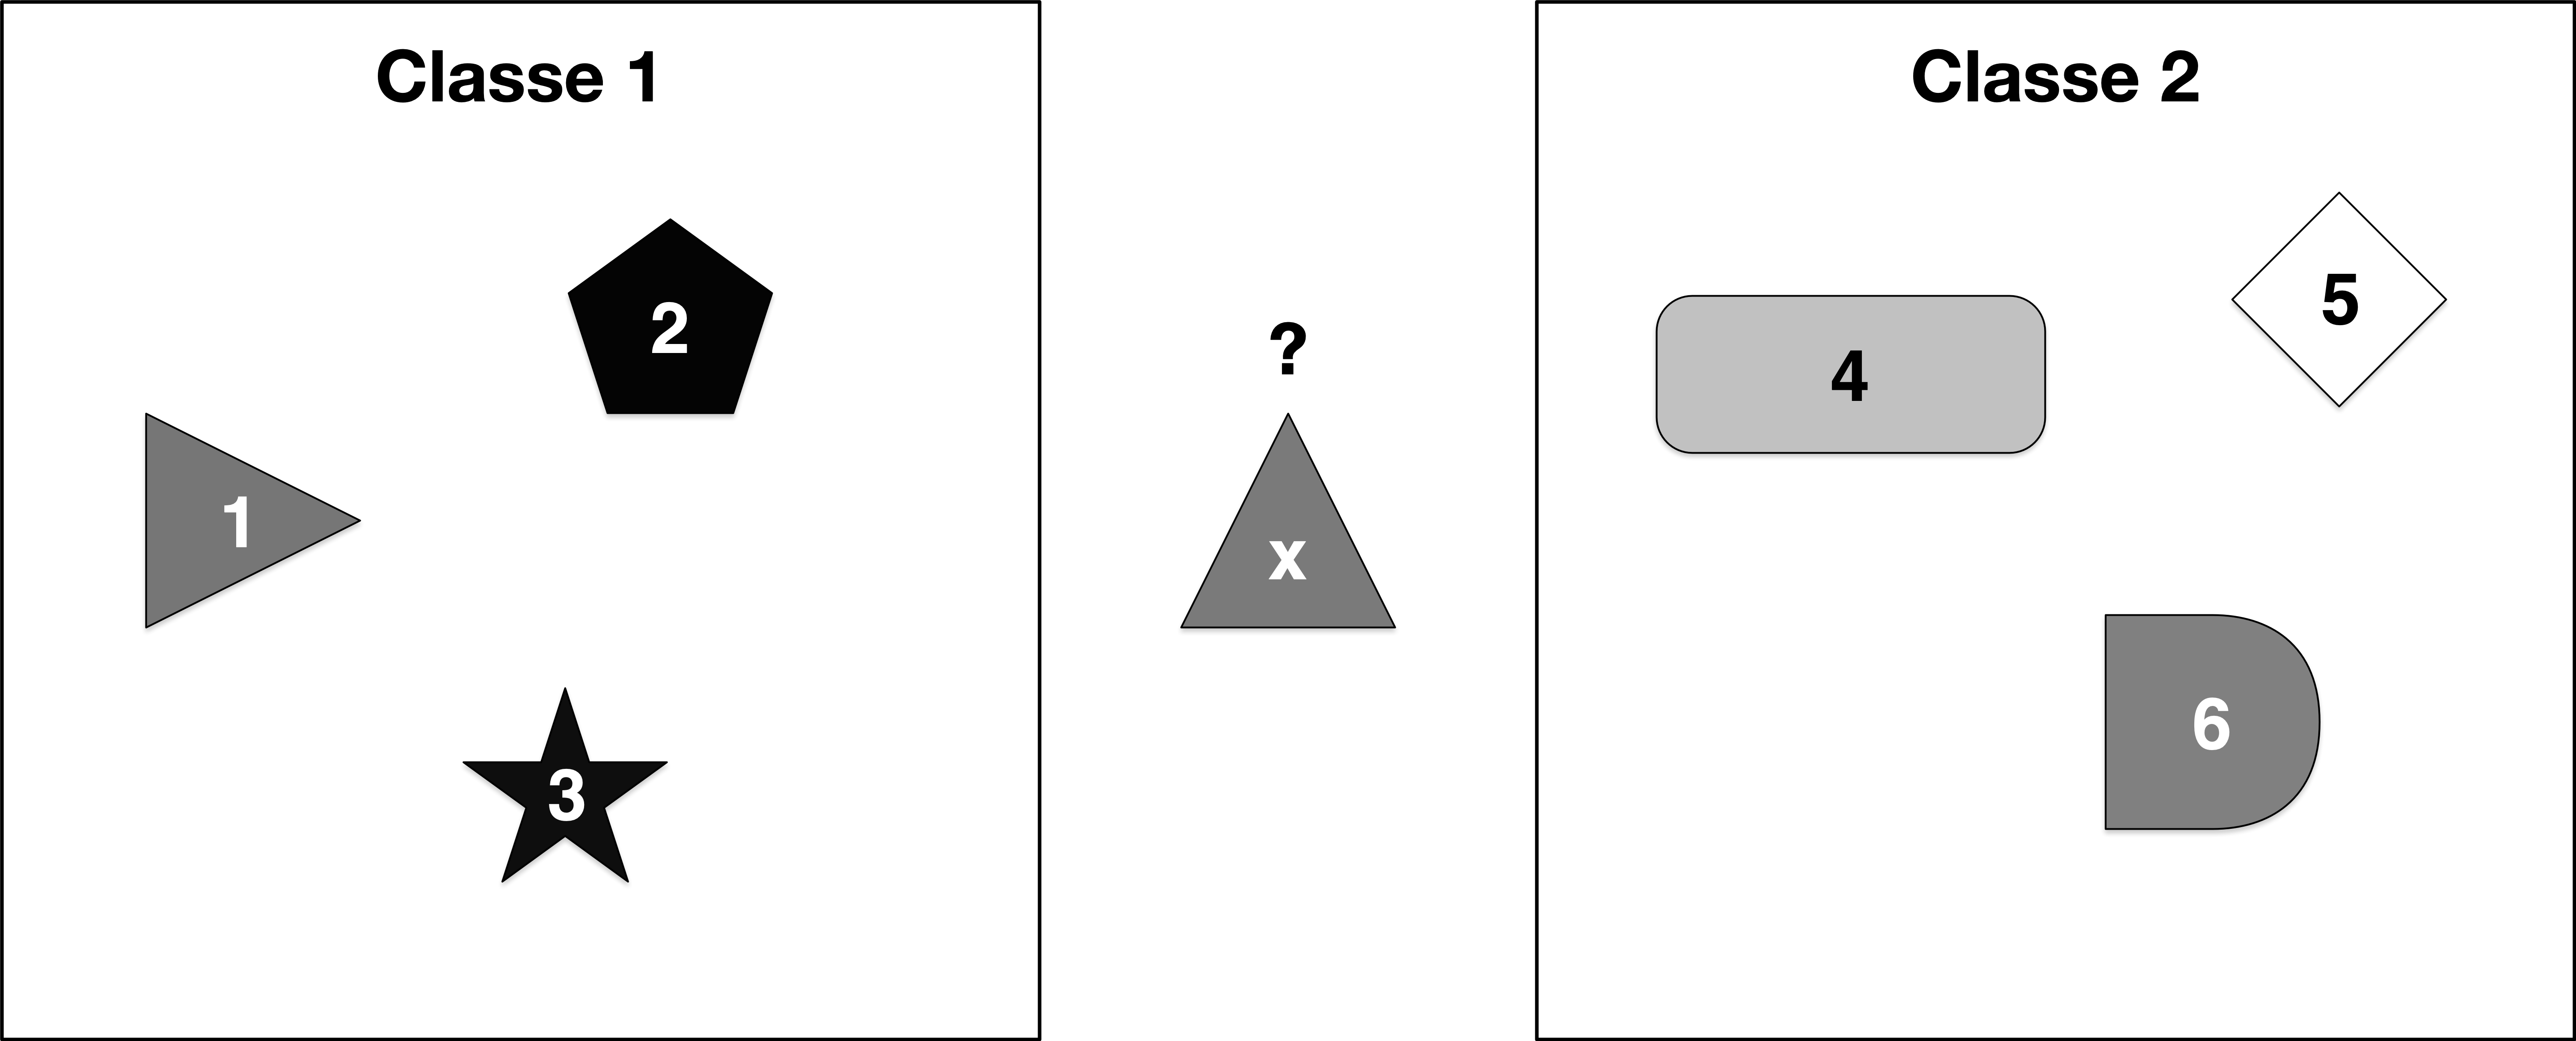
\includegraphics[scale=.09]{KRWithNewElementX.png}
    \end{center}
    \onslide<15-16>
    {\scriptsize
        \begin{itemize}[leftmargin=10pt,align=right]
            \item[\alert{\faArrowCircleRight}] Con x = $[0.48,0,0]$\\
            \onslide<16>
            %
            \[
                \begin{rcases*}
                    d(1,x) = \sqrt{(-0.01)^{2} + 0^{2} + 0^{2}} = \alert{\mathbf{0.01}} \\
                    d(2,x) = \sqrt{(-0.47)^{2} + 0.28^{2} + 0^{2}} = 0.547 \\
                    d(3,x) = \sqrt{(-0.45)^{2} + 1^{2} + 0^{2}} = 1.096 \\
                    d(4,x) = \sqrt{0.28^{2} + 0.14^{2} + 1^{2}} = 0.49 \\
                    d(5,x) = \sqrt{0.52^{2} + 0.14^{2} + 0^{2}} = 0.538 \\
                    d(6,x) = \sqrt{0.02^{2} + 0^{2} + 0^{2}} = 0.02
                \end{rcases*} C = 1
            \]
        \end{itemize}
    }
}
\only<17-18|handout:7>{
    \begin{center}
        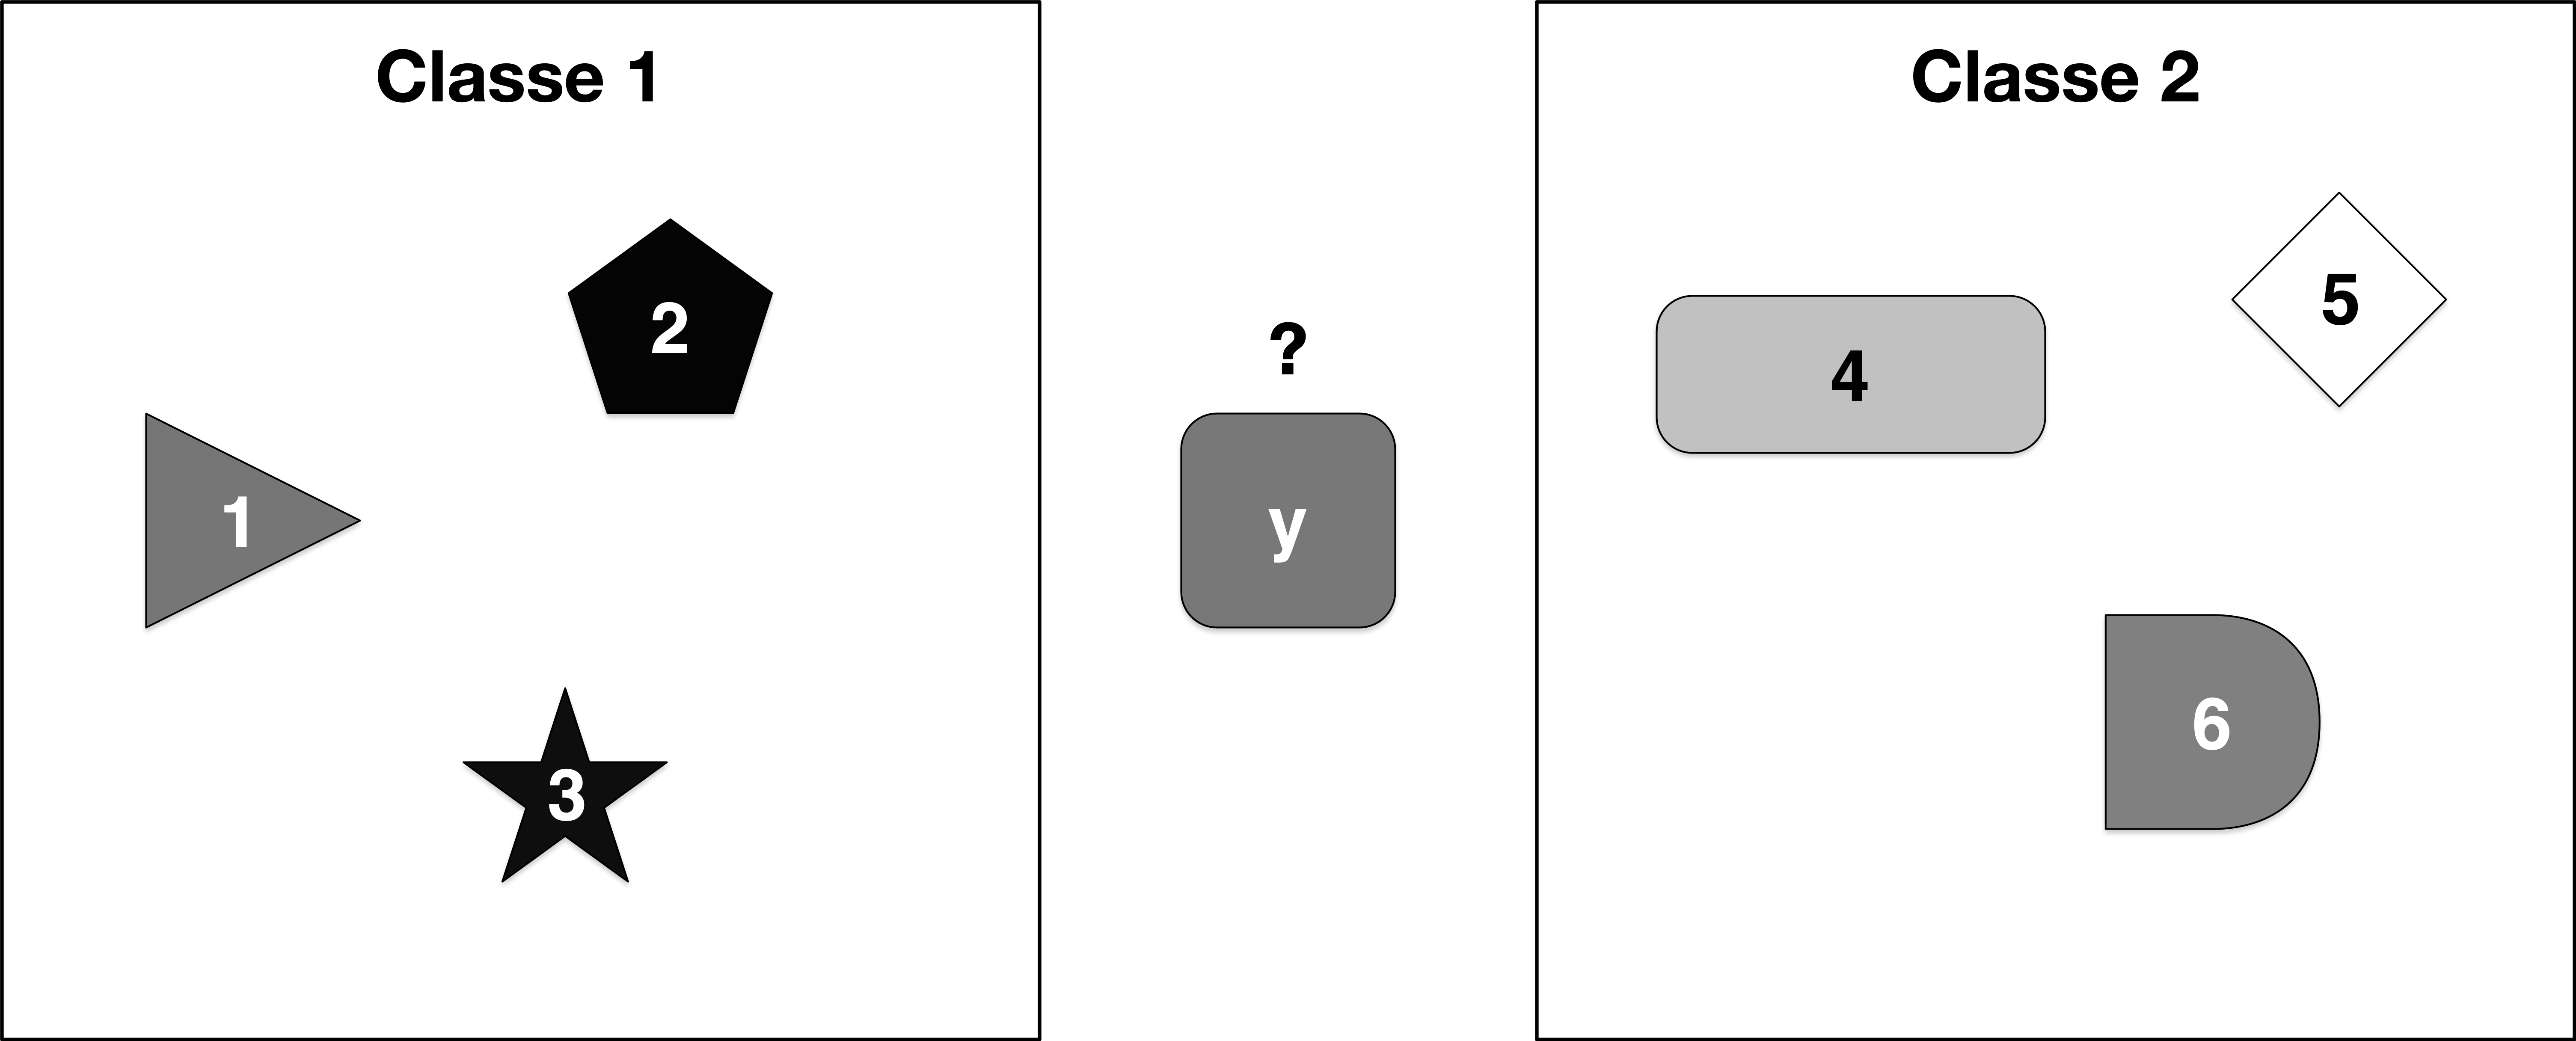
\includegraphics[scale=.09]{KRWithNewElementY.png}
    \end{center}
    \onslide<17-18>
    {\scriptsize
        \begin{itemize}[leftmargin=10pt,align=right]
            \item[\alert{\faArrowCircleRight}] Con y = $[0.47,0.14,1]$\\
            \onslide<18>
            %
            \[
                \begin{rcases*}
                    d(1,y) = \sqrt{0^{2} + (-0.14)^{2} + (-1)^{2}} = 1.009 \\
                    d(2,y) = \sqrt{(-0.46)^{2} + 0.14^{2} + (-1)^{2}} = 1.109 \\
                    d(3,y) = \sqrt{(-0.44)^{2} + 0.86^{2} + (-1)^{2}} = 1.73 \\
                    d(4,y) = \sqrt{0.29^{2} + 0^{2} + 0^{2}} = 0.289 \\
                    d(5,y) = \sqrt{0.53^{2} + 0^{2} + (-1)^{2}} = 1.131 \\
                    d(6,y) = \sqrt{0.03^{2} + 0^{2} + 0^{2}} = \alert{\mathbf{0.03}}
                \end{rcases*} C = 2
            \]
        \end{itemize}
    }
}
\end{frame}
%
\begin{frame}[b] \frametitle{\emph{Workflow} processo di \emph{Machine Learning}}
    \framesubtitle{Esempio forme geometriche}
    \begin{center}
        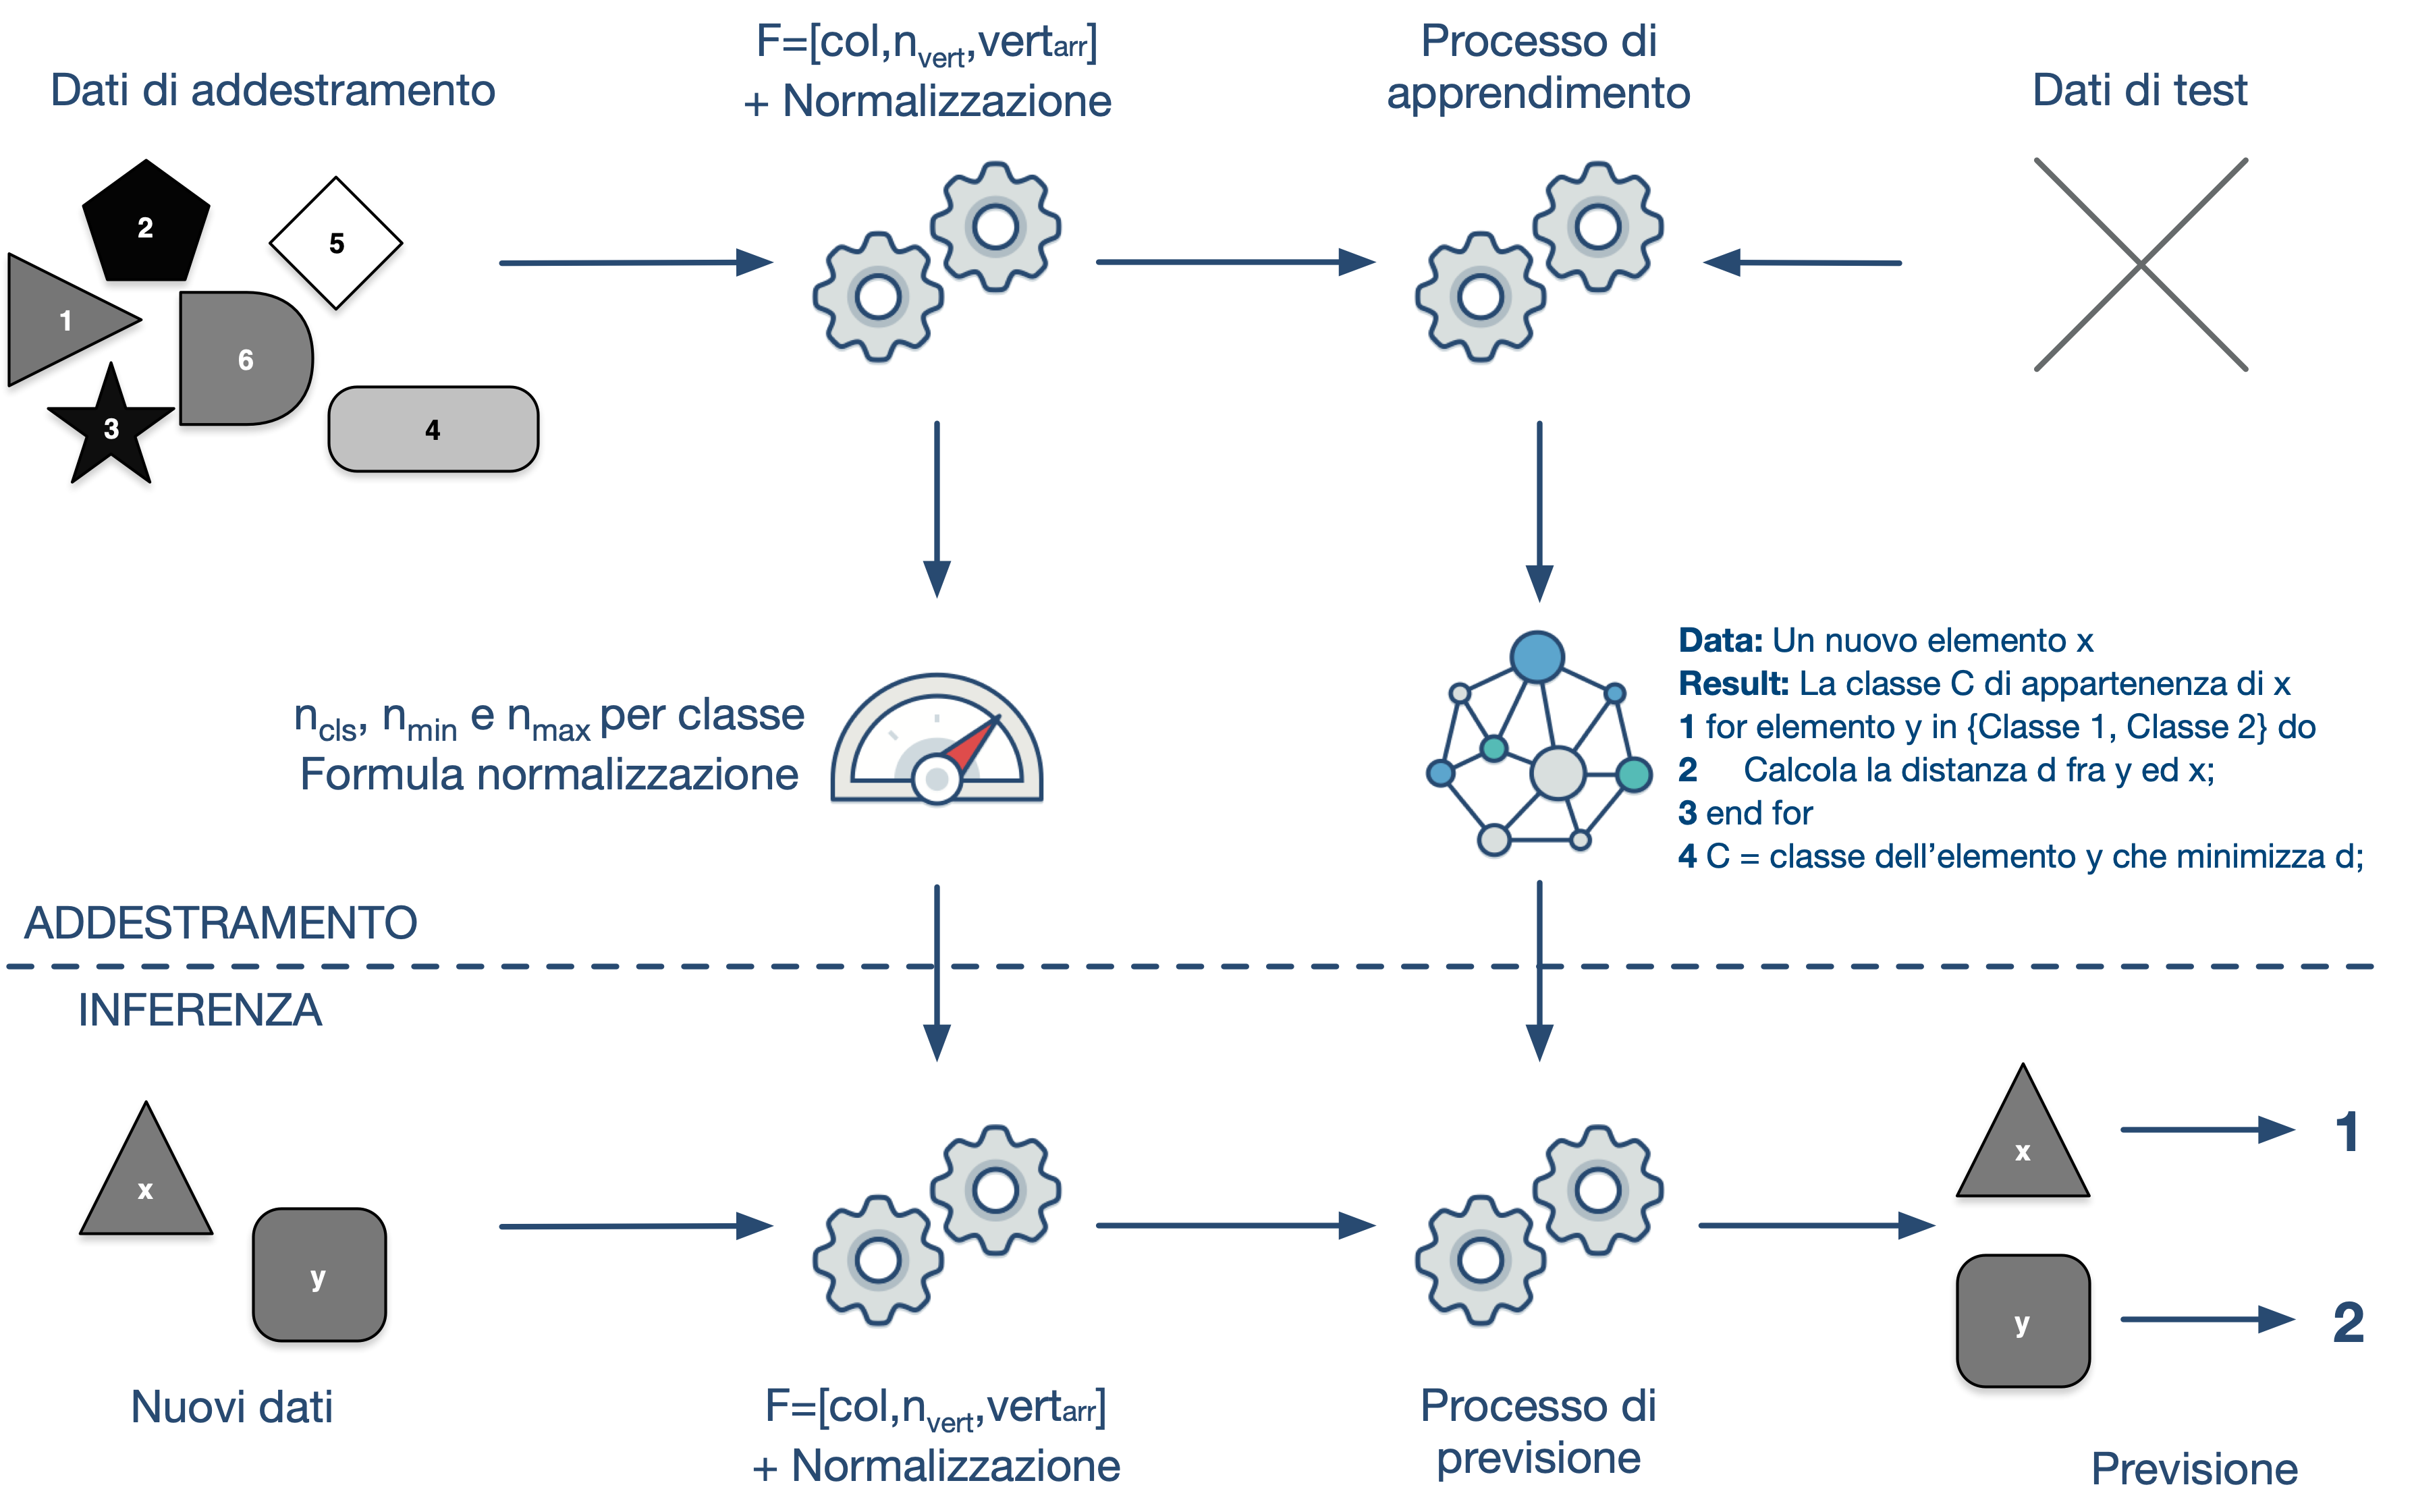
\includegraphics[height=6cm,keepaspectratio]{MLWithParametersSimpleExample.png}
    \end{center}
    \begin{flushright}
        {\tiny\textit{\textcopyright Simone Scannapieco}}
    \end{flushright}    
\end{frame}
